%--------------------------------------------------------------------------------------------------------------------
%------------------------------------------------- Preamble ---------------------------------------------------------
\documentclass[a4paper,11pt,openright]{report}
\renewcommand{\familydefault}{\sfdefault}
\usepackage{framed}
\usepackage{color}
\definecolor{myblue}{rgb}{0,0,0.7}
\definecolor{mygrey}{rgb}{0.6,0.6,0.6}
\definecolor{myred}{rgb}{0.8,0,0}
\definecolor{myred2}{rgb}{0.7,0,0}
\usepackage[colorlinks=false,citecolor=myblue,linkcolor=myblue]{hyperref}
%\usepackage[center]{subfigure}
\usepackage{graphics,graphicx}
\usepackage[spanish]{babel}
\usepackage{newlfont}
\usepackage{amsthm}
\usepackage{amsfonts}
\usepackage{amssymb}
\usepackage{amsmath}
%\usepackage{mathdots}
\usepackage{booktabs}
\usepackage{longtable}
\usepackage{lscape}
\usepackage{multirow}
\usepackage{natbib}
\usepackage[utf8]{inputenc}
\usepackage{fancyhdr}
\usepackage[dvips]{graphicx}
%\usepackage{wrapfig} 
%\usepackage{fancyhdr,epsfig}
%\usepackage{colortbl}
%\usepackage{a4wide}
%\usepackage{amssymb}
%\usepackage[latin1]{inputenc}
%\usepackage[spanish]{babel}
\DeclareGraphicsExtensions{.bmp,.png,.pdf,.jpg,.eps}



\bibpunct{\textcolor{myblue}{(}}{\textcolor{myblue}{)}}{\textcolor{myblue}{;}}{a}{\textcolor{myblue}{,}}{\textcolor{myblue}{,}}


% ---- graphics file types -----

%\DeclareGraphicsExtensions{.png}

% ------- Fonts --------
%\usepackage[T1]{fontenc}
% Cambia el formato y posici{\'o}n de las divisiones del documento
%\usepackage{sectsty}
%\allsectionsfont{\sffamily\mdseries}

% ------------- Fancy Chapters ---------------
\usepackage[Sonny]{fncychap}
%Sonny, Lenny, Glenn, Conny, Rejne and Bjarne.
\ChNameVar{\fontencoding{T1}
  \fontfamily{cmss}
  \fontseries{m}
  \fontshape{n}
  \fontsize{30}{12}
  \selectfont}
\ChNumVar{\fontencoding{T1}
  \fontfamily{cmss}
  \fontseries{m}
  \fontshape{n}
  \fontsize{30}{12}
  \selectfont}
\ChTitleVar{\fontencoding{T1}
  \fontfamily{cmss}
  \fontseries{m}
  \fontshape{n}
  \fontsize{30}{12}
  \selectfont}

% ------------------------------ Page Layout ------------------------------------

\usepackage[a4paper,text={13cm,24cm},bindingoffset=2cm,top=3cm,twoside]{
geometry }


%\usepackage[a4paper,left=5cm,top=3cm,right=2cm,twoside]{geometry}

%---------------------- Fancy Header ------------------------
\usepackage{fancyhdr}
\pagestyle{fancy} \fancyhead{} \fancyfoot{}
\renewcommand{\sectionmark}[1]{\markright{\thesection.\ #1}}
%\fancyhead[R]{\textbf{\thepage}}
%\fancyhead[L]{\nouppercase{\textbf{\rightmark}}}
\fancyhead[LE,RO]{\nouppercase{\textbf{\rightmark}}}
\fancyhead[LO,RE]{}
\fancyfoot[LE,RO]{\textbf{\thepage}}
\fancyfoot[LO,RE]{}
\renewcommand{\headrulewidth}{0.3pt}
\renewcommand{\footrulewidth}{0.3pt}


% ----------------------------------- Draft Version Stamp --------------------------------------------
\usepackage[draft,time,scrtime]{prelim2e}
\renewcommand{\PrelimWords}{\normalsize\fontfamily{augie}\selectfont\color{myred}Versi{\'o}n Borrador: 1.0}
%
\renewcommand{\thefootnote}{\textrm{\alph{footnote}}}

%--- Tree Diagram ---
\usepackage{dirtree}
\DeclareGraphicsExtensions{.bmp,.png,.pdf,.jpg,.eps}
\usepackage{graphics,graphicx}
\usepackage{wrapfig} 

%\setglossgroup{A}{Abreviaciones}%
%\setglossgroup{S}{S{\'\i}mbolos}

%\newcommand{\mydrop}[1]{\setbox0\vbox{\noindent\fontsize{30}{30}\selectfont\noindent #1}
%\wd0=0pt\ht0=0pt\box0 \hangindent=6mm\hangafter =-4\vspace{-3mm} \normalsize\noindent}

%%%%%%%%%%%%%%%%%%%%%%%%%%%% Setting to control figure placement
% These determine the rules used to place floating objects like figures
% They are only guides, but read the manual to see the effect of each.
   \renewcommand{\topfraction}{.99}
   \renewcommand{\bottomfraction}{.99}
   \renewcommand{\textfraction}{.01}
%\parindent=1.3cm
%\parindent=2cm
%\parskip=1cm

\newtheorem{defi}{{\sc Definición}}
\newtheorem{ejemplo}{\rule{0.3in}{0.11in} {\rm Ejemplo }}
\textwidth=13cm

%-----------Formato Codigo----------
\usepackage{listings}
\lstset{basicstyle=\fontfamily{augie}}




%
%\includeonly{titlepage,acknowledgements,abstract,glossary,variables,Ch0/chap0} %,Appendix/appendix5,Appendix/appendix6} %,Ch2/chap2,Ch3/chap3} %Appendix/appendixa}
%
\begin{document}
% ----- cambia enunciado Cuadros por Tabla -----------
\renewcommand{\tablename}{Tabla}
\renewcommand{\listtablename}{\'{I}ndice de tablas}

% ---P\'{a}gina de t\'{\i}tulo ---
%--------------------------------------------------------------------------------------------------------------------
%------------------------------------------------- Title Page -------------------------------------------------------
\thispagestyle{empty}
%******************************************TITLE PAGE***************************************************************
\begin{titlepage}
\begin{center}
\begin{tabular}{lr}
\multirow{4}{2.5cm}{
\includegraphics[width=2.5cm,height=2.5cm]{unrlogo}}
                                                  &  \large Universidad Nacional De Rosario (UNR)\\
                                                  &  Facultad De Ciencias Exactas, Ingenier{\'\i}a Y Agrimensura\\
                                                  &  Centro Internacional Franco Argentino de Ciencias de la\\
                                                  &  Informaci{\'o}n y Sistemas (CIFASIS). CONICET--UPCAM--UNR\\
                                                  &  Grupo de Inform{\'a}tica Aplicada a Ingenier{\'\i}a de Procesos
                                                  (GIAIP)
\end{tabular}
\end{center}
\vspace{2cm}
\begin{center}
\huge Tesis Doctoral\\
\vspace{1cm} \huge{\textbf{Desarrollo De Sistemas De Diagn{\'o}stico De Fallas Integrado Al Dise{\~n}o De Control
Tolerante A Fallas En Procesos
Qu{\'\i}micos}}\\
\vspace{2cm}
\huge David Alejandro R. Zumoffen\\
\vspace{2cm}
\end{center}
\begin{flushright}
\begin{tabular}{rl}
\large \textbf{Director:}& Dra. Marta S. Basualdo\\
\large \textbf{Co-Director:}& Dr. Mario A. Jord{\'a}n\\
&\\
&\\
\large \textbf{Miembros del jurado:}& Dr. Carlos Ruiz\\
                                    & Mst. Juan Nachez\\
                                    & Dr. Miguel Mussati\\
\end{tabular}
\end{flushright}
\vspace{1cm}
\begin{center}
\large Tesis presentada en la Facultad de Ciencias Exactas, Ingenier{\'\i}a y Agrimensura, en cumplimiento
parcial de los requisitos para optar al t{\'\i}tulo de:\\
\vspace{1cm} \huge Doctor en Ingenier{\'\i}a\\
\vspace{1cm} \normalsize 3 de Octubre de 2008
\end{center}
\end{titlepage}

\pagenumbering{roman}

%----------------------------- P\'{A}GINA DE CERTIFICACI\'{O}N --------------------------------------------------
\thispagestyle{empty}%
Certifico que el trabajo incluido en esta tesis es el resultado de tareas de investigaci\'{o}n originales y que
no ha sido presentado para optar a un t\'{\i}tulo de postgrado en ninguna otra
Universidad o Instituci\'{o}n.\\
\vspace{1cm}
\begin{flushright}
\large\fontfamily{augie}\selectfont
David Alejandro R. Zumoffen \\
\normalsize\sffamily
\end{flushright}
\vspace{15cm}
\begin{flushleft}
\setlength\fboxrule{0.8pt}\setlength\fboxsep{2mm}%
\begin{tabular}{ll}
\multirow{2}{1.8cm}{\fontfamily{augie}\selectfont\huge GIAIP \small}
                                        & \small Grupo de Inform\'{a}tica Aplicada a Ingenier\'{\i}a de Procesos.\\
                                        & \small CIFASIS (UNR-UPCAM-CONICET).\\
                                        & \small RMN - Planta Alta.\\
                                        & \small Blvd. 27 de Febrero 210 Bis.\\
                                        & \small 2000 Rosario, Argentina.\\
                                        & \small TE: +54 - 0341 - 4821771 Ext. 104.\\
                                        & \small E-mail: zumoffen@cifasis-conicet.gov.ar\\
                                        & \small A\~{n}o: 2008.
\end{tabular}
\end{flushleft}
%--------------------------------------------------------------------------------------------------------

% --------- Archivo Agradecimientos -----------
\addcontentsline{toc}{chapter}{Agradecimientos}
%--------------------------------------------------------------------------------------------------------------------
%------------------------------------------------- Acknowledgements -------------------------------------------------
\chapter*{Agradecimientos}
\emph{Primero es lo primero y no siempre en ese orden...,} en definitiva un comienzo con agradecimientos y
reconocimientos a todas las personas que directa e indirectamente han participado de este proceso parece ser
el m{\'a}s apropiado, necesario e inevitable.

Primeramente quiero expresar mi agradecimiento a mi directora de tesis la Dra. Marta Basualdo por su
inagotable fuente de paciencia. Sus directrices fueron los cimientos de todo el proceso. A mi co-director de
tesis el Dr. Mario Jord{\'a}n por su gran aporte en el {\'a}rea de control adaptivo predictivo y su excelente
predisposici{\'o}n.

Mencionar y agradecer la hospitalidad del pueblo espa{\~n}ol y en particular de la Universidad Polit{\'e}cnica de
Madrid (UPM) en mi primer a{\~n}o de doctorado en esa ciudad. Especialmente al profesor y amigo Francisco
Ballesteros Olmo del departamento de Matem{\'a}tica Aplicada a las Tecnolog{\'\i}as de la Informaci{\'o}n quien me brind{\'o}
su apoyo incondicional.

Al grupo de Sistemas Inteligentes del IFIR, principalmente al Dr. Alejandro Ceccatto por facilitar el desarrollo de esta tesis y dar el marco
necesario de trabajo.  A los compa{\~n}eros del viejo espacio f{\'\i}sico: Ulises (Uli, volv{\'e} que el barrio te est{\'a} esperando), Alejandro (Rebi), In{\'e}s y a el
Dr. Granito por el apoyo.

Quiero agradecer especialmente a los nuevos compa{\~n}eros del nuevo espacio f{\'\i}sico: Gonzalo, Jos{\'e}, Ale y Leo
por generar un lugar de trabajo insuperable y sus contribuciones en el campo de la filosof{\'\i}a. A los
directivos del Centro Internacional Franco-Argentino de Ciencias de la Informaci{\'o}n y de Sistemas (CIFASIS),
al Dr. Ceccatto y el Dr. Kaufmann, por permitir el desarrollo de este trabajo en dicho centro.

Al Consejo Nacional de Investigaciones Cient{\'\i}ficas y T{\'e}cnicas (CONICET) y a la Agencia Nacional de Promoci{\'o}n
Cient{\'\i}fica y Tecnol{\'o}gica por el soporte econ{\'o}mico en el desarrollo de {\'e}sta tesis. Tambi{\'e}n quiero agradecer
la excelente predisposici{\'o}n del caballero Carlos Franco en la resoluci{\'o}n expeditiva de problemas.

Y finalmente a mis afectos. Este espacio quiero dedicarlo especialmente a las personas que atesoro en lo
profundo de mi coraz{\'o}n. Mis viejos, mi hermana, mis amigos de siempre (Guille, Juan y Mauricio) y las dos
personas m{\'a}s importantes de mi vida, mi mujer Bel{\'e}n que me ha guiado, aguantado y estimulado en todo este
proceso (sin su enorme sentido com{\'u}n qui{\'e}n sabe por d{\'o}nde estar{\'\i}a volando)... gracias amor!. Y a mi peque{\~n}o
y hermoso beb{\'e}, Ian, que hace que cada d{\'\i}a sea una odisea de sensaciones.

\fontfamily{augie}\selectfont
\begin{flushright}
David A. Zumoffen
\end{flushright}
\sffamily


% --------- Archivo Resumen -----------
\addcontentsline{toc}{chapter}{Resumen}
%------------------------------------------------------------------------------------------------------------
%------------------------------------------------- Abstract -------------------------------------------------
\chapter*{Resumen}
En las {\'u}ltimas tres d{\'e}cadas se ha incrementado notablemente el inter{\'e}s en sistemas de monitoreo aplicado a
grandes plantas qu{\'\i}micas . Esto es debido esencialmente a condiciones de operaci{\'o}n m{\'a}s exigentes de los
procesos debido a cuestiones de seguridad de equipos y personas, costos operativos y restricciones
ambientales. La creciente complejidad en aspectos vinculados al dise{\~n}o de grandes plantas y su
correspondiente pol{\'\i}tica de control hace que los sistemas de monitoreo resulten cada vez m{\'a}s sofisticados en
aspectos tales como velocidad de detecci{\'o}n, robustez, facilidad de explicaci{\'o}n, requerimientos de modelado y
almacenamiento de datos, adaptabilidad, etc.. Esta fuerte interacci{\'o}n entre informaci{\'o}n y acciones de
control tiene lugar fundamentalmente a trav{\'e}s de sensores y actuadores. Sin embargo, estos elementos son
potenciales fuentes de fallas comunes en procesos industriales. En este contexto, se advierte que el {\'a}rea de
sistemas de monitoreo integrados al control tolerante a fallas, aplicado a plantas qu{\'\i}micas completas, es
a{\'u}n un problema abierto. En la actualidad, se han encontrado s{\'o}lo algunas soluciones particularizadas
dependientes del caso de aplicaci{\'o}n (en general acad{\'e}micos).

En tal sentido, el objetivo de esta tesis es abordar el problema de dise{\~n}o de sistemas de detecci{\'o}n,
diagnostico y estimaci{\'o}n de fallas (SDDEF) integrados al control tolerante a fallos (CTF) en procesos
qu{\'\i}micos. El desarrollo est{\'a} focalizado en automatizar el correcto manejo de situaciones anormales (MSA) y
brindar una correcta interacci{\'o}n con el usuario y la pol{\'\i}tica de control existente. El tratamiento del
problema distingue claramente las herramientas que deben emplearse de acuerdo con la dimensi{\'o}n del mismo.
As{\'\i}, se presentan soluciones alternativas para una sola unidad de proceso y varias de ellas fuertemente
interconectadas. En todos los casos se contemplan a los sistemas bajo esquemas de control convencional y
avanzado. El desarrollo de un novedoso SDDEF, apto para plantas de diferentes dimensiones y contemplando los
requerimientos fundamentales que impone hoy la industria qu{\'\i}mica constituye uno de los principales aportes
de esta tesis. Herramientas tales como transformada wavelet discreta, identificaci{\'o}n de sistemas, an{\'a}lisis
de componentes principales, sistemas de l{\'o}gica difusa y redes neuronales artificiales son integradas
adecuadamente para el desarrollo del SDDEF. En este contexto se presenta una nueva metodolog{\'\i}a general para
el correcto MSA en grandes procesos basado en un SDDEF h{\'\i}brido y estrategias de integraci{\'o}n al CTF activo,
ya sea de pol{\'\i}ticas de control existentes o nuevas.  El SDDEF se dise{\~n}a de forma tal que resulte
independiente de factores tales como, dimensi{\'o}n, complejidad, operabilidad y tipo de los procesos y de sus
estrategias de control.

Esta tesis est{\'a} organizada como sigue: el cap{\'\i}tulo 1 presenta el marco de referencia de los problemas reales
encontrados habitualmente en procesos industriales y sus consecuencias. El cap{\'\i}tulo 2 presenta una extensa
recopilaci{\'o}n bibliogr{\'a}fica que permite adquirir un panorama amplio del estado del arte en el abordaje de
MSA, dise{\~n}o de sistemas de monitoreo y CTF desde el punto de vista acad{\'e}mico e industrial. El cap{\'\i}tulo 3
realiza una breve descripci{\'o}n de las principales herramientas utilizadas a lo largo de esta tesis tanto en
el campo del procesamiento de la informaci{\'o}n como del {\'a}rea de control de procesos. El cap{\'\i}tulo 4 aborda el
problema principalmente orientado a unidades aisladas de proceso que contemplan menor n{\'u}mero de variables.
Aqu{\'\i} se presentan los principales resultados obtenidos en la aplicaci{\'o}n de control predictivo adaptivo como
CTF activo. Dado que se confrontan los resultados alcanzados con y sin sistema de diagn{\'o}stico, es posible
realizar una evaluaci{\'o}n rigurosa de los alcances de emplear el SDDEF integrado al CTF.Se discuten aqu{\'\i}
dise{\~n}os basados en la TWD e identificaci{\'o}n de sistemas para la conformaci{\'o}n del SDDEF. Los resultados
obtenidos provienen tanto de planteos te{\'o}ricos como de un caso de aplicaci{\'o}n de un reactor tipo tanque
agitado continuo con camisa. Adem{\'a}s, se proponen nuevas alternativas de control adaptivo predictivo,
pol{\'\i}ticas de integraci{\'o}n y manejo de eventos anormales en lazos simples de control. Fallas t{\'\i}picas como
offset en sensores y retardos extras en actuadores son analizadas de forma secuencial y simple, en paralelo
con diferentes condiciones de operaci{\'o}n de los procesos. El cap{\'\i}tulo 5 presenta el dise{\~n}o de un complejo
SDDEF h{\'\i}brido para procesos de grandes dimensiones y su integraci{\'o}n al CTF para pol{\'\i}ticas de control
existentes. La estrategia propuesta es probada sobre casos de aplicaci{\'o}n tales como una planta de
tratamiento de aguas residuales y una de pulpa y papel (la cual representa el caso m{\'a}s complejo y de mayor
dimensi{\'o}n existente en la comunidad de investigaci{\'o}n de control de procesos). Adem{\'a}s, se desarrollan varios
{\'\i}ndices capaces de brindar una correcta evaluaci{\'o}n ya sea de funcionamiento del SDDEF, as{\'\i} como de costos
involucrados con el empleo del SDDEF integrado al CTF. Se presenta un  conjunto importante de simulaciones
efectuadas en diferentes escenarios para poder apreciar el aporte concreto de esta estrategia. Fallas en
sensores del tipo offset y en actuadores del tipo retardo extra y bloqueos son propuestas. Las fallas
consideradas en cada caso de estudio fueron seleccionadas acorde con la magnitud del problema que produc{\'\i}an
las mismas. De esta forma se considera que la metodolog{\'\i}a propuesta se somete a pruebas contundentes que
posibilitan extraer sustentar las conclusiones presentadas en el cap{\'\i}tulo 6. En el mismo tambi{\'e}n se incluyen
algunas posibles direcciones futuras de trabajos de investigaci{\'o}n. Finalmente, los ap{\'e}ndices dan el soporte
necesario a tem{\'a}ticas espec{\'\i}ficas como identificaci{\'o}n recursiva con factor de olvido, predicciones con
diferentes modelos lineales, algoritmos de factorizaci{\'o}n, control basado en modelo interno y control en
avance.

Durante el desarrollo de esta tesis se han generado diversas publicaciones, las cuales han sido sometidas tanto a arbitrajes nacionales como
internacionales. Los trabajos m{\'a}s importantes se resumen en el cap{\'\i}tulo denominado publicaciones (y en anexo al final de la tesis).


% --------- Archivo Publicaciones -----------
\addcontentsline{toc}{chapter}{Publicaciones}
%------------------------------------------------------------------------------------------------------------
%------------------------------------------------- Publicaciones --------------------------------------------
\chapter*{Publicaciones}
Durante el desarrollo de esta tesis se han generado diversas publicaciones. Las principales se detallan a continuaci{\'o}n:
\begin{enumerate}
\small
    \item[A-] \textbf{An Approach to Improve the Performance of Adaptive Predictive Control Systems: Theory,  Simulations and Experiments.} M.
        Jord{\'a}n, M. Basualdo and D. Zumoffen. \textit{International Journal
    Of Control}. 2006, 79(10), 1216/1236.
    \item[B-] \textbf{Robust Adaptive Predictive Fault-Tolerant Control Linked with Fault Diagnosis System Applied On a Nonlinear Chemical Process.} D.
        Zumoffen, M. Basualdo, M. Jord{\'a}n and A. Ceccatto.
    \textit{Proceedings of the 45th IEEE Conference on Decision and Control}. 2006, 3512/3517. San Diego,
    CA, USA.
    \item[C-] \textbf{Robust Adaptive Predictive Fault-Tolerant Control Integrated To a Fault-Detection System Applied to a Nonlinear Chemical
        Process.} D. Zumoffen, M. Basualdo, M. Jord{\'a}n and A.
    Ceccatto. \textit{Ind. Eng.
    Chem. Res.}. 2007, 46(22), 7152/7163.
    \item[D-] \textbf{From Large Chemical Plant Data to Fault Diagnosis Integrated to Decentralized Fault-Tolerant Control: Pulp Mill Process
        Application.} D. Zumoffen and M. Basualdo. \textit{Ind. Eng.
    Chem. Res.}. 2008, 47(4), 1201/1220.
    \item[E-] \textbf{Improvements in Fault Tolerance Characteristics for Large Chemical Plants Part I: Waste Water Treatment Plant with Decentralized
        Control}. D. Zumoffen and M. Basualdo. \textit{Ind. Eng. Chem. Res.}. 2008, 47(15), 5464/5481.
    \item[F-] \textbf{Improvements in Fault Tolerance Characteristics for Large Chemical Plants Part II: Pulp Mill Process with Model Predictive Control.} D.
        Zumoffen, M. Basualdo and G. Molina. \textit{Ind. Eng. Chem. Res.}. 2008, 47(15), 5482/5500.
\end{enumerate}
\normalsize

Las publicaciones A, B y C forman parte del cap{\'\i}tulo 3 y la estructura fundamental del cap{\'\i}tulo 4. A su vez las publicaciones D, E y F estructuran el
cap{\'\i}tulo 5. En cada caso, dichos cap{\'\i}tulos pretenden otorgar un visi{\'o}n extendida de las publicaciones documentando nuevos resultados y estrategias.

Adem{\'a}s, numerosos trabajos interdiciplinarios se han llevado a cabo en este per{\'\i}odo. El resultado de dicha interacci{\'o}n se ve reflejada en las
publicaciones enunciadas anteriormente y los siguientes trabajos presentados en congresos y reuniones cient{\'\i}ficas:
\begin{enumerate}
\small \item \textit{Desarrollo De Un Sensor Virtual De Composiciones Para La Implementaci{\'o}n De Control
 Con Trayectoria {\'O}ptima Aplicado A Destilaci{\'o}n Batch.} J.P. Ruiz, F. Garetto, D. Zumoffen y M.
 Basualdo. Congreso X RPIC, Argentina. 2003.

\item \textit{A Nonlinear Soft Sensor For Quality Estimation And Optimal Control Applied In A Ternary Batch Distillation Column.} J.P. Ruiz, D.
Zumoffen, M. Basualdo and L. Jimenez  Esteller. ESCAPE 14 European Symposium on Computer Aided Process Engineering, Portugal. 2004.

\item \textit{Aplicaci{\'o}n De Control Predictivo Funcional Para El Seguimiento De Una Trayectoria {\'O}ptima De Temperatura En Una Columna De Destilaci{\'o}n
Batch Multicomponente.} D. Zumoffen, L. Garyulo y M. Basualdo. XIX Congreso Argentino de Control Autom{\'a}tico, Argentina. 2004.

\item \textit{Predictive Functional Control Applied To Multicomponent Batch Distillation Column.} D. Zumoffen, L. Garyulo, M. Basualdo and L.
Jim{\'e}nez. ESCAPE 15, European Symposium on Computer Aided Process Engineering, Spain. 2005, 1465/1470.

\item \textit{Sistema De Detecci{\'o}n De Fallas En Un CSTR Controlado Con PFC.} D. Zumoffen, M. Basualdo y A. Ceccatto. Congreso XI RPIC, Argentina.
2005.

\item \textit{Control Tolerante Predictivo Funcional aplicado A Un CSTR.} D. Zumoffen, M. Basualdo y M. Jord{\'a}n. Congreso XI RPIC, Argentina. 2005.

\item \textit{Control predictivo generalizado no lineal aplicado a una columna de destilaci{\'o}n batch ternaria.} J. Walczuk, L. Caviglia, D. Zumoffen y
M. Basualdo. Congreso XI RPIC, Argentina. 2005.

\item \textit{On the Design of Fault-Tolerant Systems using Robustness Filtering with Adaptive Control.} M. Jord{\'a}n, M. Basualdo and D. Zumoffen.
Congreso XI RPIC, Argentina. 2005.

\item \textit{An Industrial Application Of Signal Processing For Developing A Fault Diagnosis System Linked With A Fault Tolerant Control Strategy.}
M. Basualdo and D. Zumoffen. Workshop on Signal Processing (WSP06), Argentina. 2006.

\item \textit{Control Tolerante A Fallos Integrado A Un Sitema De Diagnosis Basado En An{\'a}lisis De Principales Componentes Y L{\'o}gica Difusa.} D.
Zumoffen, M. Basualdo y G. Molina. XX  Congreso Argentino de Control Autom{\'a}tico, Argentina. 2006.

\item \textit{Fault Detection and Estimation System Integrated To Fault Tolerant Control. Part I: FDIE System Design.} D. Zumoffen and M. Basualdo.
Congreso XII RPIC, Argentina. 2007.

\item \textit{Fault Detection and Estimation System Integrated To Fault Tolerant Control. Part II: Reconfiguration of the Control Strategy.} D.
Zumoffen and M. Basualdo. Congreso XII RPIC, Argentina. 2007.

\item \textit{Hybrid Fault Diagnosis For Large Chemical Plants Under Control.} D. Zumoffen and M. Basualdo. ESCAPE 18, European Symposium on Computer
Aided Process Engineering, France. 2008.

\item \textit{Fault Diagnosis and Identification System Applied to a Non-invasive Biosensor of Blood Glucose.} M. Basualdo, D. Zumoffen and A.
Rigalli. ESCAPE 18, European Symposium on Computer Aided Process Engineering, France. 2008.

\item \textit{Monitoreo Y CTF en Grandes Plantas Qu{\'\i}micas. Parte I: Dise{\~n}o del SDDEF.} D. Zumoffen y M. Basualdo. XXI Congreso Argentino de Control
Autom{\'a}tico, Buenos Aires, Argentina. 2008.

\item \textit{Monitoreo Y CTF en Grandes Plantas Qu{\'\i}micas. Parte II: Integraci{\'o}n al CTF.} D. Zumoffen y M. Basualdo. XXI Congreso Argentino de
Control Autom{\'a}tico, Buenos Aires, Argentina. 2008.
\end{enumerate}
\normalsize


% ------------ Glosario y Variables ------------
\addcontentsline{toc}{chapter}{Glosario}
%--------------------------------------------------------------------------------------------------------------------
%------------------------------------------------- Glossary -------------------------------------------------
\chapter*{Glosario}
\begin{longtable}{rl}
 ACP   & An{\'a}lisis en componentes principales\\
 ACPA  & An{\'a}lisis en componentes principales adaptivo\\
 ACPD  & An{\'a}lisis en componentes principales din{\'a}mico\\
 ACPM  & An{\'a}lisis en componentes principales m{\'o}vil\\
 ACPME & An{\'a}lisis en componentes de principales de m{\'u}ltiples escalas\\
 ACPPE & An{\'a}lisis en componentes principales pesado exponencialmente\\
 ACT   & An{\'a}lisis cualitativo de tendencias\\
 AF    & {\'A}rboles de fallas\\
 ARX   & Autorregresivo con entrada externa (AutoRegressive with eXogenous input) \\
 ASM1  & Modelo de lodos activos (Activate Sludge Model) N\textordmasculine 1\\
 BTO   & Beneficio total de operaci{\'o}n \\
 CAPFRA& Control adaptivo predictivo con filtro robusto adaptivo\\
 CBMI  & Control basado en modelo interno\\
 CEA   & Control en avance (feedforward)\\
 CFRAP & Control con filtro robusto adaptivo predictivo\\
 COD   & Concentraci{\'o}n de ox{\'\i}geno disuelto\\
 CPA   & Control predictivo adaptivo\\
 CPF   & Control predictivo funcional\\
 CPM   & Control predictivo multivariable\\
 CTF   & Control tolerante a fallos\\
 DDF   & Detecci{\'o}n y diagnostico de fallas\\
 DG    & Digrafos\\
 DGS   & Digrafos con signo\\
 DVS   & Descomposici{\'o}n en valores singulares\\
 EAR   & Extracci{\'o}n autom{\'a}tica de reglas\\
 ECP   & Error cuadr{\'a}tico de predicci{\'o}n\\
 ECMP  & Error cuadr{\'a}tico medio de predicci{\'o}n\\
 FC    & F{\'\i}sica cuantitativa\\
 FEC   & Filtros espejo en cuadratura\\
 FIR   & Respuesta finita al impulso (Finite Impulse Response)\\
 FP    & Funci{\'o}n de pertenencia\\
 IEA   & Integral del error absoluto\\
 IS    & Identificaci{\'o}n de sistemas\\
 LB    & Licor blanco \\
 LD    & L{\'o}gica difusa\\
 LF    & L{\'\i}nea de fibra\\
 LND   & Licor negro d{\'e}bil\\
 LV    & Licor verde \\
 MCP   & M{\'\i}nimos cuadrados parciales\\
 MMPE  & Media m{\'o}vil pesado exponencialmente\\
 MRG   & Matriz relativa de ganancias \\
 MSA   & Manejo de situaciones anormales\\
 OD    & Ox{\'\i}geno disuelto\\
 P     & Control proporcional\\
 PA    & Promedio de los autovalores\\
 PI    & Control proporcional/integral\\
 PID   & Control proporcional/integral/derivativo\\
 PMB   & Porcentaje de mejora del beneficio\\
 PME   & Porcentaje de mejora del error\\
 PPP   & Planta de pulpa y papel\\
 PQ    & Punto de quiebre\\
 PSR   & Porcentaje de soporte de la regla\\
 PTAR  & Planta de tratamiento de aguas residuales\\
 PTD   & Porcentaje del tiempo de detecci{\'o}n\\
 PVA   & Porcentaje de varianza acumulado\\
 RNA   & Redes neuronales artificiales\\
 RQ    & Recupero qu{\'\i}mico \\
 RTAC  & Reactor tanque agitado continuo\\
 SA    & Situaci{\'o}n anormal\\
 SCTF  & Sistema de control tolerante a fallos\\
 SDDEF & Sistema de detecci{\'o}n, diagnostico y estimaci{\'o}n de fallas\\
 SDEF  & Sistema de detecci{\'o}n y estimaci{\'o}n de fallas\\
 SE    & Sistema experto\\
 SISO  & Simple entrada/simple salida (Single Input/Single Output)\\
 SLD   & Sistema de l{\'o}gica difusa\\
 SM    & Sistema de monitoreo\\
 SVD   & Subespacio de variaci{\'o}n dominante\\
 TWD   & Transformada wavelet discreta\\
 UO    & Unidades en capa oculta\\
 US    & Unidades en capa de salida\\
 VC    & Variable controlada\\
 VM    & Variable manipulada\\
\end{longtable}

\addcontentsline{toc}{chapter}{Variables}
%--------------------------------------------------------------------------------------------------------------------
%------------------------------------------------- Variables -------------------------------------------------
\chapter*{Variables}
\small
\section*{Cap{\'\i}tulo 2}
\begin{tabular}{rlrl}
$d(k)$ & Se{\~n}al de perturbaci{\'o}n &&\\
$f(k)$ & Evoluci{\'o}n temporal de la falla &&\\
$u(k)$ & Se{\~n}al de entrada &&\\
$y(k)$ & Se{\~n}al de salida &&\\
$\hat{f}(k)$ & Estimaci{\'o}n de la falla &&\\
$y_{ref}(k)$ & Trayectoria de referencia &&\\
\end{tabular}
\section*{Cap{\'\i}tulo 3}
\begin{tabular}{rlrl}
$\mathbf{1}_{m}$ & Vector de unos de longitud $m$            & $\mu_i$ & Valor medio de la variable $i$\\
$a$ & Escalado wavelet                                       & $\sigma_i$ & Varianza de la variable $i$\\
$A$ & Componentes principales                                & $\lambda_i$ & Autovalor $i$ \\
$\mathbf{A}$ & Matriz del modelo EE                          & $\Delta \bar{\mathbf{x}}$ & Error de predicci{\'o}n\\
$A_J$ & Aproximaci{\'o}n a nivel $J$                             & $\delta_{T^2}$ & L{\'\i}mite de confianza para $T^2$\\
$b$ & Desplazamiento wavelet                                 & $\delta_{Q}$ & L{\'\i}mite de confianza para $Q$\\
$\mathbf{b}$ & Vector de valores medios                      & $\chi^2$ & Distribuci{\'o}n chi-cuadrado\\
$\mathbf{B}$ & Matriz del modelo EE                          & $\nu$ & Factor de confianza\\
$C(a,b)$ & Coeficientes wavelets                             & $\psi(\cdot)$ & funci{\'o}n wavelet madre\\
$D_j(t)$ & Detalle a nivel $j$                               & $\phi(\cdot)$ & funci{\'o}n de escala\\
$D^*(z^{-1})$ & Polinomio causal                             & $\theta$ & Vector de par{\'a}metros\\
$\mathbf{D}_{\lambda}$ & Matriz de autovalores               & $\hat{\theta}$ & Vector de par{\'a}metros estimado\\
$\mathbf{D}_{\lambda A}$ & Matriz de $A$ autovalores         & $\alpha^{(i)}$ & Paso en la iteraci{\'o}n $i$ \\
$\mathbf{e}(k)$ & Vector de errores                          & $\xi^{(i)}$ & Direcci{\'o}n de b{\'u}squeda en $i$\\
$\mathbf{E}$ & Matriz de restricciones                       & $\theta^{(i)}$ & Estima en $i$ \\
$f_i(\cdot)$ & Funci{\'o}n de pertenencia $i$                    & $\theta^{0}$ & Valor inicial de la estima\\
$F(z^{-1})$ & Filtro pasa bajo                               & $\varphi_j$ & Entrada $j$ de la neurona\\
$F_{A,m-A,\alpha}$ & Distribuci{\'o}n $F$                        & $\phi(k)$ & Regresor lineal\\
$\mathbf{F}$ & Matriz de restricciones                       & $\varepsilon(N)$ & Error de predicci{\'o}n a priori\\
$g(i)$ & Coeficientes del modelo FIR                         & $\epsilon(k)$ & Error de seguimiento \\
$G$ & Filtro pasa alto wavelet                               & $\alpha_i$ & Pesos del error\\
$\tilde{G}$ & Filtro espejo de $G$                           & $\beta_i$ & Pesos del control\\
$G(z^{-1})$ & Transf. del proceso                            & $\Delta \hat{u}(k)$ & Movimiento futuro de control\\
$\hat{G}(z^{-1})$ & Transf. estimada del proceso             & $\eta(k)$ & Perturbaci{\'o}n de salida\\
$\hat{G}_0(z^{-1})$ & Transf. estimada nominal del proceso   & $\hat{\eta}(k)$ & Estimaci{\'o}n de la perturbaci{\'o}n\\
$\mathbf{G}$ & Matriz de restricciones                       & $\Delta \hat{\mathbf{U}}(k)$ & Movimientos futuros \\
$h_p$ & Fin horizonte de predicci{\'o}n                          & $\Delta \hat{G}(z^{-1},k)$ & Correcci{\'o}n del modelo\\
$h_u$ & Horizonte de control                                 & $\Delta \hat{\theta}(k)$ & Correcci{\'o}n de los
par{\'a}metros
\end{tabular}

\begin{tabular}{rlrl}
$h_w$ & Inicio horizonte de predicci{\'o}n &&\\
$H$ & Filtro pasa bajo wavelet &&\\
$\tilde{H}$ & Filtro espejo de $H$ &&\\
$J(k)$ & Funcional costo matricial &&\\
$K(N)$ & Ganancia del algoritmo MCR &&\\
$K_g$ & Compensaci{\'o}n est{\'a}tica &&\\
$n$ & no. variables medidas &&\\
$n_h$ & no. neuronas en capa oculta &&\\
$n_\varphi$ & no. de entradas &&\\
$pva(l)$ & \% de varianza acumulada para $l$ &&\\
$\mathbf{P}$ & $A$ componentes principales &&\\
$\bar{\mathbf{P}}$ & subespacio residual &&\\
$\mathbf{P}_N$ & Inversa de la matriz de correlaci{\'o}n &&\\
$Q(k)$ & Estad{\'\i}stico ECP &&\\
$r(t)$ & Ruido de medici{\'o}n &&\\
$R(z)$ & Polinomio no causal &&\\
$\mathbf{R}$ & Matriz de correlaci{\'o}n &&\\
$s(t)$ & Se{\~n}al para an{\'a}lisis wavelet &&\\
$\mathbf{s}$ & Vector de varianzas &&\\
$t$ & Tiempo &&\\
$\mathbf{t}(k)$ & Variables latentes &&\\
$T_{ref}$ & Tiempo de respuesta &&\\
$T_s$ & Tiempo de muestreo &&\\
$T^2(k)$ & Estad{\'\i}stico de Hotelling &&\\
$\mathbf{T}_1$,$\mathbf{T}_2$,$\mathbf{T}_3$,$\mathbf{T}_4$ & Matrices de transformaci{\'o}n &&\\
$u(k)$ & Se{\~n}al de entrada &&\\
$\hat{\mathbf{u}}(k)$ & Vector de entradas futuras &&\\
$\mathbf{U}$ & Vector de movimientos futuras &&\\
$V_N(\cdot)$ & funcional costo cuadr{\'a}tico &&\\
$w_{ij}$ & Peso $j$ de la neurona $i$ &&\\
$w_{i0}$ & Bias de la neurona $i$ &&\\
$w(k)$ & Trayectoria de referencia &&\\
$x(k)$ & Estados del modelo EE &&\\
$\bar{\mathbf{x}}$ & Medici{\'o}n normalizada del proceso &&\\
$X$ & Espacio de entrada &&\\
$\mathbf{X}$ & Matriz de datos &&\\
$\bar{\mathbf{X}}$ & Matriz de datos normalizada &&\\
$y(k)$ & Se{\~n}al de salida &&\\
$y_i$ & Salida de la neurona $i$ &&\\
$\hat{y}_i$ & Predicci{\'o}n de $y_i$ &&\\
$\hat{\mathbf{y}}(k)$ & Vector de predicciones &&\\
$\mathbf{Y}_r$ & Vector de referencias futuras &&\\
$Z^N$ & Datos entrada/salida con $N$ muestras &&
\end{tabular}

\section*{Cap{\'\i}tulo 4}
\begin{tabular}{rlrl}
$\hat{d}(k)$ & Retardo estimado            &$\alpha_r$ & Cte. tiempo filtro\\
$G_{vm}(z^{-1})$ & Modelo actuador/v{\'a}lvula &$\phi_{au}$& Regresor aumentado\\
$h(k)$ & Respuesta al escal{\'o}n              &$\hat{\theta}_{au}$& Estima aumentada\\
$o_{ff}(t)$ & Offset de medici{\'o}n           &$\zeta$& Umbral del retardo\\
$p_o(k)$ & Valor de pico en $D_1$          &$\lambda$& Factor de olvido\\
$\hat{ppo}$ & Par{\'a}metro de punto operativo &$\delta_o$& Par{\'a}metro proporcional\\
$r(t)$ & Ruido de medici{\'o}n                 &&\\
$s_1(k)$ & Versi{\'o}n filtrada de $z_n(k)$    &&\\
$t_d$ & Retardo temporal                   &&\\
$T_f$ & Tiempo de ocurrencia de la falla   &&\\
\end{tabular}

\begin{tabular}{rl}
$u_{00}$ & Punto operativo de la entrada\\
$u_c(t)$ & Se{\~n}al de control \\
$u_c(t-t_d)$ & Se{\~n}al de control retrasada en $t_d$ \\
$w_0(k)$ & Referencia original\\
$y(t)$ & Variable de salida real \\
$y_m(t)$ & Variable de salida medida \\
$y_{00}$ & Punto operativo de la salida\\
$z_n(k)$ & Indicador de persistencia a la excitaci{\'o}n
\end{tabular}

\section*{Cap{\'\i}tulo 5}
\begin{tabular}{rlrl}
$\mathbf{b}_{VM_j}$ & Valor medio de la $VM_j$             &$\delta_z$& L{\'\i}mite de confianza para $z$\\
$BTO_j^i$ & Beneficio total de operaci{\'o}n                   &$\delta_{pva}$ & \% de varianza acumulada\\
$\bar{c}_i$ & Precio costo/venta                           &$\tau_f^i$ & Cte. de tiempo filtro CBMI\\
$ECMP_j$ & Error cuadr{\'a}tico medio de predicci{\'o}n            &$\eta$ & Par{\'a}metro de dise{\~n}o \\
$fp_j^i$ & Funci{\'o}n de pertenencia $j$ sobre $i$            &$\mu$ & Conversi{\'o}n de unidades\\
$F_i$ & Falla tipo $i$                                     &$\tau_m$ & Cte. tiempo del modelo\\
$\bar{F}_i^j$ & Cantidad de material                       &$\kappa_i$ & Par. del modelo inferencial\\
$IEA_j^i$ & Integral del error absoluto                    &$\upsilon_i$ & Par. del modelo inferencial\\
$K_m$ & Ganancia del modelo                                &$\tau_p$ & Cte. tiempo del proceso\\
$K_p$ & Ganancia del proceso                               &$\theta_p$ & Tiempo muerto del proceso\\
$K_{PI}$ & Ganancia del PI                                 &$\tau_{PI}$ & Cte. integral del PI\\
$l_i$ & Valor ling{\"u}{\'\i}stico para $i$                         &&\\
$[L_{min}^i,L_{max}^i]$ & Rango de operaci{\'o}n normal de $i$ &&\\
$M_i$ & Modelo inferencial $i$ &&\\
$N_a$ & N{\'u}mero m{\'a}ximo de alertas de peligro &&\\
$N_{aux}$ & Dimensi{\'o}n matriz auxiliar &&\\
$N_{w}$ & Dimensi{\'o}n matriz normal &&\\
$\hat{o}_{ff}^{VC_j}$ & Estimaci{\'o}n del offset en $VC_j$ &&\\
$p$ & N{\'u}mero de reglas &&\\
$PI_i$ & Controlador PI del lazo $i$ &&\\
$PMB_j^i$ & Porcentaje de mejora del beneficio &&\\
$PSR_j$ & Porcentaje de soporte de la regla $j$ &&\\
$PTD$ & Porcentaje de tiempo de detecci{\'o}n &&\\
$r$ & N{\'u}mero de componentes de $\mathbf{u}_{FL}$ &&\\
$\mathbf{R}_p$ & Regla del evento $p$ &&\\
$\mathbf{R}_{matriz}$ & Matriz de reglas &&\\
$\mathbf{s}_{VC_j}$ & Varianza de la $VC_j$ &&\\
$s_i$ & Activaci{\'o}n del lazo adicional $i$ &&\\
$sp_i(k)$ & Referencia para $i$ &&\\
$sp_i^0(k)$ & Referencia original para $i$ &&\\
$sp_{pr}^0(k)$ & Ref. original de producci{\'o}n &&\\
$sp_{pr}^1(k)$ & Ref. actualizada de producci{\'o}n &&\\
$\hat{t}_d^{VM_j}$ & Estimaci{\'o}n del retardo en $VM_j$ && \\
$T_c$ & Tiempo de clasificaci{\'o}n &&\\
$T_d$ & Tiempo de detecci{\'o}n &&\\
$[T_{iz},T_{fz}]$ & Zona de an{\'a}lisis &&\\
$T_r$ & Tiempo de reconfiguraci{\'o}n &&\\
$T_{sd}$ & Din{\'a}mica mas lenta del proceso &&\\
$T_u$ & Tiempo de actualizaci{\'o}n &&\\
$u_{FL}(k)$ & Entradas del SLD &&\\
$u_i^m$ & Valor medio de $i$ &&\\
$u_i^c$ & Correcci{\'o}n de la ref. de producci{\'o}n &&\\
$\mathbf{u}_{FL}^m$ & Vector de contribuciones medias &&
\end{tabular}

\begin{tabular}{rl}
$V_a(k)$ & Funcional costo adicional \\
$V_0(k)$ & Funcional costo original \\
$VA$ & \% de violaci{\'o}n de amon{\'\i}aco \\
$VN$ & \% de violaci{\'o}n de nitr{\'o}geno \\
$\bar{\mathbf{X}}_{n}$ & Matriz de datos normales\\
$\bar{\mathbf{X}}_{aux}$ & Matriz auxiliar\\
$y_i^m(k)$ & Medici{\'o}n de la salida $i$\\
$\hat{y}_i^m(k)$ & Inferencia de la salida $i$\\
$\mathbf{y}_{FL}$ & Salida del SLD\\
$z(k)$ & Estad{\'\i}stico combinado\\
\end{tabular}

\section*{Ap{\'e}ndices}
\begin{tabular}{rlrl}
$\mathbf{A}$ & Matriz del modelo EE            &$\lambda$& Factor de olvido\\
$\mathbf{B}$ & Matriz del modelo EE            &$\xi$& Retardo del proceso\\
$\mathbf{C}$ & Matriz del modelo EE            &$w$& Frecuencia\\
$C(s)$ & Transferencia del controlador &&\\
$\mathbf{D}_*$ & Matriz de la factorizaci{\'o}n UD &&\\
$e_m$ & Error multiplicativo &&\\
$f_{lp}(s)$ & Transferencia del filtro pasa bajos &&\\
$\tilde{g}_+(s)$ & Parte no invertible &&\\
$\tilde{g}_+(s)$ & Parte invertible &&\\
$G(s)$ & Transferencia del proceso &&\\
$\tilde{G}(s)$ & Modelo del proceso &&\\
$G_c(s)$ & Transferencia del CBMI &&\\
$\mathbf{G}$ & Matriz din{\'a}mica &&\\
$K_{ff}$ & Transf. del controlador en avance &&\\
$\mathbf{S}$ & Matriz din{\'a}mica &&\\
$u(k)$ & Se{\~n}al de entrada &&\\
$\mathbf{U}_*$ & Matriz de la factorizaci{\'o}n UD &&\\
$x(k)$ & Estados del modelo EE &&\\
$y(k)$ & Se{\~n}al de salida &&\\
\end{tabular}
\normalsize


% ---- Lista de contenidos, figuras y tablas ----
\tableofcontents \listoffigures \listoftables

% -- Archivo Cap\'{\i}tulo N� 0 --
%-------------------------------------------------------------------------------
--------------------------------
%------------------------------------------------- Chapter 1 --------------------------------------------------------
\parskip=0.6cm

\chapter{Introducción}\label{cap:1} 
%\label{cap:introduccion}
%\pagenumbering{arabic}


\begin{abstract}
ggfgfd

\end{abstract}


\section{introducción}

El objeto de estudio de la presente tesis surgió en el marco de un grupo interdisciplinario de I+D del CONICET-UNR que se dedica a investigar problemáticas de integración de las Tecnologías de la Información y Comunicación (TIC) en contextos organizacionales de Educación Superior. Así, en esta tesis se sostiene una perspectiva computacional acorde al contexto, totalmente integrada a los postulados del Programa de Investigación, Desarrollo y Transferencia "Dispositivos Hipermediales Dinámicos" radicado en el CIFASIS (CONICET-UNT-UPCAM) bajo la dirección de la Dra. Patricia San Martín.

Así, la presente investigación iniciada en el año 2005 y con vigencia hasta nuestros días, tiene como objetivo principal atender a los requerimientos de mayor flexibilidad y dinamismo de los entornos e-learning. En otras palabras, se desarrolla una propuesta para la incorporación (agregado) de propiedades de adaptación dinámicas, reconfiguración e inteligencia (AdRI) \label{AdRI} a los servicios bases del framework Sakai,
especialmente diseñadas para implementar los proceso en ambientes e-learning (Pe-Colaborativos) definidos en el marco de \cite{cacic2007.9} donde se requieren nuevos aspectos de adaptación \cite{librounq} implementados a partir del framework Sakai. Dicha
implementación se ajusta a los requisitos y requerimientos(capítulo \ref{cap:1}) del Dispositivo Hipermedial Dinámico que, entendido como una red sociotécnica, posibilita a los sujetos desarrollar actividades académicas y profesionales bajo la modalidad de taller físico-virtual. 
La definición y representación del
contexto es un punto central de este trabajo que se tratará en profundidad en el
capítulo \ref{cap:estadodelarte} teniendo en cuenta que el contexto para el DHD necesita un
tratamiento específico.

Ahora bien, los primeros  desafíos  que se evidencian en el aporte de esta tesis se relacionan con la formalización de varias de las especificaciones que aquí se proponen. En este sentido, es necesario iniciar la formalización de los requerimientos de manera efectiva para captar aquellos aspectos conceptuales que determinan configuraciones particulares del DHD. Actualmente, se cuenta con un recorrido en la investigación significativo en la construcción de las especificaciones del DHD, esto se desarrolla en el capítulo \ref{cap:2} donde se citan modelos canónicos que interpretan propiedades bien definidas para su descripción formal.

En el trayecto del textual de la tesis se hace más presente que las problemáticas sobre adaptabilidad dinámica, reconfiguración e inteligencia \hyperref[AdRI]{(AdRI)} están fuertemente orientadas a la construcción de reglas, lo cual implica que eventualmente pueden existir limitaciones importantes para su manipulación. En este sentido, el estudio está enfocado en cuestiones de diseño e implementación en las que se puedan lograr instancias del sistema cuya configuración resuelva cuestiones funcionales manteniendo las
características de AdRI descriptas en las secciones \ref{sec:motivacion} y \ref{sec:solucion}.

Los mencionados requerimientos se enfocaron a mejorar la calidad y las posibilidades de desarrollo de los procesos educativos, de investigación y de producción hipermedial bajo la modalidad de un espacio colaborativo web en la modalidad físico-virtual. Esto permitió elaborar las primeras hipótesis de la presente investigación, delimitando así los alcances del estudio a la Ingeniería de Software y a las Ciencias de la Computación aplicada a la interpretación de la complejidad de estos requerimientos y su correspondiente infraestructura de resolución. Los saberes, aprendizajes y experiencias previas del autor de la presente investigación doctoral, fueron claves para llevar a cabo exitosamente los requerimientos planteados, ya que dicha tarea demandó la realización de un estudio específico de proyectos centrados especialmente en el campo del “e-learning'', desde una mirada interdisciplinaria. 

A partir de las indagaciones efectuadas en el estado del arte, pudo verificarse que los sistemas colaborativos se mostraban como una propuesta racional para sostener modelos donde se podían implementar soluciones tecnológicas para aquellos requerimientos funcionales que derivasen de un requisito de más alto nivel en los que aumenta el grado de subjetividad, ya que es necesario tener en cuenta aspectos relativos al contexto, tipos de relaciones y vínculos que dan lugar a diferentes niveles de complejidad e interpretación.
 
Desde hace más de 10 años, se evidencia un creciente interés por metodologías de trabajo más efectivas, que tomen en cuenta el potencial, los intereses y las particularidades de cada uno de los sujetos. Se busca generar conocimiento útil a partir de la información disponible y del desarrollo de competencias que permitan aplicar, posteriormente, ese conocimiento de manera efectiva. No obstante, la complejidad de la problemática afrontada requiere del trabajo mediante diversos grupos, constituidos por personas capaces de interactuar de forma sinérgica para buscar soluciones adecuadas y con alto grado de creatividad \cite{cap1.1}. La construcción de conocimiento aplicando metodologías de diálogo interdisciplinar ha dejado de ser una opción para convertirse en una necesidad. Esto, sumado al rol protagónico de las TIC en la actual Sociedad de la Información y del Conocimiento y, el vertiginoso desarrollo que han tenido en los últimos años, se han planteado paradigmas y esquemas de trabajo que integran a las ciencias computacionales con otros campos del conocimiento tales como las ciencias humanas y sociales, las ciencias administrativas, el diseño gráfico y artístico, etc.; han llevado a la construcción de un nuevo contexto físico-virtual pero, reconociendo al tiempo, que pese al potencial de las TIC, gran parte de los problemas a resolver, no pueden ser abordados exclusivamente desde una perspectiva exclusivamente tecnológica \cite{cap1.2,cap1.3}. Así, este trabajo afrontó un desafío: colaborar desde las Ciencias de la Computación al despliegue del diálogo y de la producción interdisciplinar del grupo de trabajo sobre el campo conceptual referido a la integración de TIC en los procesos de aprendizajes denominados PodA \label{ProdA}. Se los puede caracterizar a partir de diferentes estadíos de acciones de usuarios y transacciones del sistema  integrados (figura \ref{fig:Proda}) de forma conjuntas y jerárquicas. De esta manera, un proceso ProdA está compuesta por la primera fase donde un usuario o computadora proveerá información a la aplicación, por ejemplo un docente autorizado de un espacio TIC. Luego, una segunda fase corresponde a todas las actividades referida al consumo y utilización de esa información,  por ejemplo: actividades que desempeñan los alumnos. En tercer lugar se encuentran las transacciones, herramientos y procedimientos destinado a la evaluación de conocimientos adquiridos,  por ejemplo: los alumnos realizan exámenes dentro del espacio colaborativa que permita clasificar los resultados para que puedan intervenir usuarios autorizados para complementar las evaluaciones.  En el cuarto y quinto lugar se encuentran las influencias sobre las cuestiones metodológicas y tecnológicas del contexto.



\begin{figure}
 
\begin{center}
 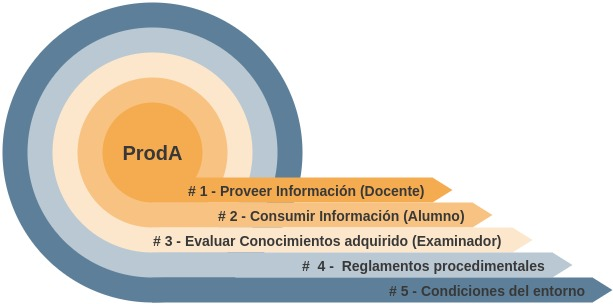
\includegraphics[scale=0.55]{Ch0/ProdA.jpg}
 % arqDHD.: 450x422 pixel, 72dpi, 15.88x14.89 cm, bb=0 0 450 422
\label{fig:proda}
\caption{Componentes que integran el proceso ProdA.} 
\end{center}

\end{figure}




De esta manera, a lo largo del proceso de investigación doctoral, se construyó teórica y metodológicamente, de manera consensuada, una categoría denominada "Dispositivo Hipermedial Dinámico" – en adelante DHD- (San Martín, et. al, 2008).  


\begin{defi}

Se conceptualiza al Dispositivo Hipermedial Dinámico (DHD) como una red heterogénea [3] conformada por la conjunción de tecnologías y aspectos sociales -red sociotécnica- que en el actual contexto físico-virtual posibilita a los sujetos realizar acciones de interacción responsable con el otro para investigar, enseñar, aprender, dialogar, confrontar, diseñar, componer, evaluar, producir, diseminar, transferir, bajo la modalidad de taller, utilizando la potencialidad comunicacional, transformadora y abierta de lo hipermedial, regulados según el caso por un “coordinación de contratos”. \cite{arqDHD20}

\end{defi}



\section{Publicaciones de Apoyo}

De esta manera, la definición de DHD está avalada en las siguientes publicaciones de apoyo. Además, la mayor parte de los avances de esta tesis ya fueron publicados en libros prologados, revistas con referato y memorias de conferencias y congresos, registrándose a la fecha algunas publicaciones en prensa o revisión.

Los primeros aportes, en los cuales se comienza a desarrollar una noción
sobre la inyección de contratos en una plataforma e-learning, se describen en
el capítulo ``Implementaciones de entornos e-learning en la formación de
arquitectos. Hacia una aplicación context-aware dinámica físico-virtual'' Capítulo XIII en Rodríguez Barros, Diana. (Comp.) Experiencia Digital. Usos, prácticas y estrategias en talleres de arquitectura y diseño en entornos virtuales. Mar del
Plata, Universidad de Mar del Plata, 2006, pp. 195-204.

El marco teórico y metodológico interdisciplinar que fundamenta la construcción del concepto DHD fueron publicados en los capítulos 5 "Sistemas Context-Aware en dispositivos hipermediales dinámicos para educación e investigación”, y 6 "Los contratos
context-aware en aplicaciones para educación e investigación", del libro Hacia un Dispositivo Hipermedial Dinámico: Educación e investigación para el campo audiovisual interactivo \cite{librounq}, (San Martín, Sartorio, Guarnieri y Rodríguez). En el primer capítulo, se describe una primera aproximación de la arquitectura conceptual de un DHD con propiedades de sensibilidad del contexto. En el segundo capítulo, se introduce la
primera noción de los contratos sensibles al contexto y se propone un mecanismo
de implementación. 

Además, las siguientes dos publicaciones completan el recorrido sobre la conceptualización del DHD, publicaciones que fueron tomadas como punto de partida para la definición de los requerimientos del DHD, propuesto en el capítulo \ref{cap1.2} 

Una de ellas es el libro El Dispositivo Hipermedial Dinámico: Campus Virtual UNR (San Martín, P.; Guarnieri, G; Rodirguez, G; Bongiovani, P.; Sartorio, A.; 2010), en donde se plantea un proceso de reconceptualización del Campus Virtual de la Universidad Nacional de Rosario (UNR), Argentina; realizado en el marco del Programa de Investigación, Desarrollo y Transferencia "Dispositivos Hipermediales Dinámicos" (CIFASIS: CONICET, UNR, UPCAM) a solicitud de la Secretaría de Tecnologías Educativas y de Gestión(UNR). El objetivo del libro estuvo centrado en promover y fortalecer estratégicamente la integración de las TIC en actividades educativas, de investigación y vinculación tecnológica en el
actual contexto físico-virtual. La metodología implementada estudió el caso
conjuntamente con los propios actores de la UNR, fundamentándose en conceptos,
métodos y bases epistemológicas de la investigación interdisciplinaria en el
marco de los sistemas complejos.

San Martín, P.; Guarnieri, G.; Sartorio, A.; Rodríguez, G. ―Construir un campus
virtual: reflexiones sobre un caso de vinculación tecnológica. Publicado en el
2008 por la Revista de la Escuela de Ciencias de la Educación. Este artículo con referato
presenta una de las primeras experiencias de implementación de la modalidad de
becario e investigador en empresa ofrecida por el Consejo Nacional de
Investigaciones Científicas y Técnicas -CONICET-, llevada a cabo durante los
años 2006 y 2007 en una organización que, si bien era de base tecnológica,
deseaba consolidar su perfil como institución educativa, ya que sus servicios
principales se centraban desde el año 2000, en la capacitación profesional para
la operatoria de softwares multimediales, desarrollo aplicaciones hipermediales
y composición hipermedial.


Otras publicaciones que colaboraron con el desarrollo conceptual del DHD fueron las siguientes publicaciones en reuniones científico-tecnológicas: 

\begin{itemize}
 \item 
Guarnieri G., Rodríguez G., Sartorio A. (2007). De la máquina de Enseñar
a las Interacciones Múltiples. Congreso sobre nuevas tecnologías y educación
(Edutec 2007), Buenos Aires, Argentina.

\item
Rodríguez G., Sartorio A., Guarnieri G. (2007). El software libre en el
campo del E-learning. Congreso sobre nuevas tecnologías y educación (Edutec
2007). Buenos Aires. Argentina.

\item
San Martín P., Sartorio A., Rodríguez G. (2006) Una mesa de arena para
Investigar y Aprender en
Contextos físicos-virtuales-interactivos-comunicacionales de Educación Superior.
Actas del XV Encuentro Internacional de Educación a distancia. UDGV.
Guadalajara, México.

\item
Sartorio A., Guarnieri G. (2006), Diseño de herramientas de Context Aware
Dinámico aplicadas a una experiencia de
taller físico-virtual-interactivo-comunicacional. Segunda edición de las
Jornadas Abiertas de Informática SADIO Rosario.

\item
En cuanto al recorrido sobre la teoría de los contratos sensibles al contexto,
su implementación y metodología de aplicación, las siguientes publicaciones (en
órden de importancia) sostienen lo expuesto a partir del
capítulo \ref{cap1.arqdhd}.

\item
Sartorio, A., Cristiá, M. (2009). First Approximation to DHD Design and
Implementation. CLEI ELECTRONIC JOURNAL.
Rodríguez G., San Martín, P., Sartorio A. (2009), Aproximación al modelado del
componente conceptual básico del Dispositivo Hipermedial Dinámico. XV Congreso
Argentino de Ciencias de la Computación.  

\item
Sartorio A., San Martín P., Rodriguez, G., Guarnieri, G. (2009), Los contratos
sensibles al contexto para los Dispositivos Hipermediales Dinámicos. Jornadas de
Ciencias de la Computación - FCEIA - UNR.

\item
Rodríguez G., Sartorio, A. (2008), Aspectos Tecnológicos y
Modelos Conceptuales de un Dispositivo Hipermedial Dinámico. Sexto
Congreso Internacional en Innovación Tecnológica Informática Universidad
Abierta Interamericana.

\item
Sartorio A., Cristiá M. (2008). Primera Aproximación al Diseño e Implementación
de los DHD.   XXXIV Conferencia Latinoamericana de Informática (CLEI 2008).

\item
Todos los aportes que se brindaron a la comunidad Sakai
\footnote{Sakai Comunnity:http://sakaiproject.org/community-overview} en la
novena conferencia junto con otros significativos trabajos: \footnote{
http://confluence.sakaiproject.org/display/CONF09/Conference+Presentations}. 

\item
Sartorio A. (2008). A conceptual framework  to apply Sakai with contract
and its practical implementation. 9th Sakai Conference Paris, France.

\end{itemize}



Los aspectos metodológicos referidas al diseño del contrato y la
detección de su ubicación en la etapa de diseño constan en los
siguientes trabajos:

\begin{itemize}
 
\item 
Sartorio, A. (2008), Un modelo comprensivo para el diseño de procesos en
una Aplicación E-Learning. XIII Congreso Argentino de Ciencias de la
Computación. CACIC 2007.

\item 
Sartorio A. (2007), Un comprensivo modelo de diseño para la integración
de procesos de aprendizaje e investigación en una Aplicación E-Learning,
Congreso sobre nuevas tecnologías y educación (Edutec, 2007), Buenos Aires, 
Argentina.

\end{itemize}


\begin{itemize}

Para el capítulo \ref{cap1.implementaciones} se utilizaron los avances sobre
el uso de métricas y tipos de condicionales a partir de las siguientes
publicaciones: 

\item  
Sartorio, A., Rodriguez, G. (2010), Condicionales DEVS en la coordinación de
contratos sensibles al contexto para los DHD. CACIC 2010. En prensa.

\item 
Rodriguez, G., Sartorio, A., San Martín, P. (2010) SEPI: una herramienta para el Seguimiento y Evaluación de Procesos Interactivos del DHD. CACIC 2010. En prensa.
Sartorio A. et al (2007), Students' interaction in an e-learning contract
context-aware application with associated metric, Actas del IATED2007,
International Technology, Education and Development Conference, IATED, Valencia,
España.

\end{itemize}

La construcción de la categoría DHD, permitió ver que la elección de metodologías y paradigmas en los que se integran tecnologías y funcionalidades conceptuales, necesitan ser interpretados como posibles instancias que se puedan configurar de acuerdo a las necesidades y navegabilidad de cada sujeto. Por lo tanto, se pueden interpretar propiedades generales de los sistemas a partir de las posibles configuraciones de un estado determinado, de un caso de uso concreto. Este análisis es tratado en el grupo de I+D “Obra Abierta: DHD para educar e investigar'' a través de la teoría de los sistemas complejos y se tiene en cuenta como ítems para la clasificación de aplicaciones colaborativas o “Groupware''.

Ahora bien, es necesario aclarar que los aspectos que se tendrán en cuenta en esta tesis sobre los sistemas colaborativos son:


\begin{itemize}

\item  Nivel de automatización: Las aplicaciones ``Groupware`` como considera
Patricia Schnaidt, se pueden clasificar de acuerdo al tipo de trabajo en grupo
que apoyan: \cite{cap1.1.groupware}

\item  {Flujo de documentos, Automatización de procesos, Automatización de
tareas, Herramientas flexibles de trabajo en grupo.}


\item De acuerdo al espacio-tiempo de los miembros del grupo: Se consideran las
aplicaciones “groupware” de acuerdo al tipo de interacción de los miembros del
grupo de trabajo \cite{cap1.4.groupware}.

\begin{itemize}
\item Interacción Sincrónica
\item Interacción Asincrónica
\item Distribución Sincrónica
\end{itemize}

\item De acuerdo al manejo de información. Según el soporte que brindan
\cite{cap1.5.groupware} los sistemas “groupware” pueden clasificarse en:
\begin{itemize}
 \item Sistemas para compartir Información
 \item Sistemas cooperativos.
 \item Sistemas concurrentes.
\end{itemize}

\item De acuerdo al propósito de la aplicación: es posible encontrar dos tipos de
aplicaciones dependiendo de su propósito.
\begin{itemize}
 \item Aplicaciones de propósito general.
 \item Aplicaciones de propósito específico.
\end{itemize}

\item De acuerdo al tipo de aplicación: Dependiendo del tipo de aplicación
y funcionalidad se pueden clasificar en los siguientes grupos:

\begin{itemize}
 \item Sistemas de mensajes por computador
 \item GDSSs (Group Decision Support Systems).
 \item Sistemas de coordinación: Orientados a la formas, orientados al proceso,
orientados al diálogo, orientados a la estructura de comunicación.	
\end{itemize}

\item De acuerdo al tipo de reconfiguración orientada a la Interactividad
DHD\cite{libro.unr}. Dependiendo del grado de expresión que se tiene para
reconfigurar el sistema teniendo en cuenta información procesada
para la representación de contexto interno y del entorno.

\begin{itemize}
 \item Reconfiguración dinámica.
 \item Adaptabilidad.
\item Sensibilidad al contexto.
\item Sistemas expertos: bases de conocimientos y motores de inferencias.
\end{itemize}

\end{itemize}


Los aportes originales de esta tesis se fundamentan a lo largo de este documento en publicaciones de circulación internacional acreditadas proponiendo una perspectiva innovadora referida a la reconfiguración dinámica de los entornos colaborativos orientada a la Interactividad en los procesos de aprendizaje \hyperref[ProdA]{(ProdA)}  en el DHD. 


\section{Motivación}\label{sec:motivacion}


Al mismo tiempo que el avance en la investigación y desarrollo de entornos colaborativos brindan mejoras e innovaciones en herramientas (videoconferencias, porfolios, wikis, workshops, etc.) y sus respectivos servicios, crece la cantidad de posibles configuraciones de los espacios colaborativos.

Estas configuraciones abarcan diferentes tipos de requerimientos pertenecientes a las  etapas de diseño, desarrollo e incluso exigen que el espacio colaborativo se ''adapte'' en tiempo de ejecución. A partir de estos requerimientos iniciales, se definen los procesos e-colaborativos, los cuales serán denominados en esta tesis como Pe-colaborativos \cite{cacic2007.7}, que son similares a los procesos de negocio en otros dominios de aplicación. La denominación de Pe-colaborativos, surge de la evolución del recorrido teórico iniciado a partir de las transacciones Web, que dieron lugar a teorizar el concepto de transacciones e-learning \cite{cacic2007} y que en el trayecto de desarrollo de esta investigación evolucionaron finalmente hacia el concepto de procesos e-colaborativos o Pe-Colaborativos como se ha denominado. 


Al igual que los procesos de negocios en una Aplicación Web convencional, los Pe-colaborativos están compuestos por transacciones Web \cite{cacic2007.7}. En este contexto, una transacción o transacción e-colaborativa, es definida como una secuencia de actividades que un usuario ejecuta a través de una Aplicación colaborativa con el propósito de efectuar una tarea o concretar un objetivo, donde el conjunto de actividades, sus propiedades y las reglas que controlan sus ejecuciones dependen del Pe-colaborativos que la Aplicación debe brindar. Un ejemplo que puede ser citado es la posibilidad de implementar una estrategia didáctica que le brinde al alumno que participa en un entorno virtual colaborativo la posibilidad de acceder a un tipo de Objeto Digital Educativo específico, dependiendo de sus intervenciones en los Foros. Estos requerimientos resultan difíciles de implementar en las actuales aplicaciones e-learning que son utilizadas a nivel global.

Las características funcionales de Aplicaciones Web Colaborativas (en adelante AW-Colaborativas), tales como Sakai \footnote{\url{http://sakaiproject.org/}}, se basan en brindar navegación entre páginas a través de links y ejecución de transacciones colaborativas desde las herramientas (por ejemplo foros, anuncios, exámenes, blogs) que utilizan los servicios de la plataforma (ej., edición, manejo de audio y vídeo, consultas, navegación, etc.).
En el marco de los análisis efectuados se observó que el proyecto Sakai brinda una de las propuestas más consolidadas relativas al diseño y al desarrollo de entornos colaborativos, teniendo en cuenta los ítems \ref{sec:motivacion} anteriormente analizados. En este sentido, la plataforma Sakai está orientada a herramientas que se implementan mediante servicios comunes (servicios bases). Una de ellas, es el servicio de edición de mensajes es utilizado en las herramientas foro, anuncio, blog, portfolio, etcétera. Otras de las características sobresalientes de Sakai es la versatilidad para su extensión y/o configuración, lo que permite alterar ciertas configuraciones  referidas al tiempo de ejecución, por ejemplo, instrumentar una nueva funcionalidad en un servicio base de Sakai.

Sin embargo, estas soluciones no pueden resolver aquellos Pe-Colaborativos que
involucren cambios en el comportamiento de las relaciones entre un componente
(cliente) que ocasiona, a través de un pedido, la ejecución de un componente
servidor (proveedor). Estos cambios refieren a la capacidad de
adaptación dinámica del sistema \cite{cacic2007.14} extendiendo, personalizando
y mejorando los servicios sin la necesidad de recompilar y/o reiniciar el
sistema. 

Cuando se refiere a las propiedades de inteligencia de un framework, se atribuye
a un entorno con características heterogéneas con numerosos
componentes de software y hardware \cite{cap1.133}. Esta diversidad implica
ciertos desafíos problemáticos que demandan una atención especial en los diseños
solicitando una preparación para usos complejos multisensoriales tales como:  

\begin{itemize} 
 
\item
Se han de integrar y gestionar distintos tipos de tecnología, con
el consecuente aumento de complejidad en el desarrollo. El usuario puede
utilizar múltiples modos (habla, gestos, tacto) para interaccionar con
el entorno, con lo que se requieren interfaces de usuario muy variadas. Por
otro lado, la distribución de la información requiere distintos tipos de redes,
según la naturaleza de ésta.

\item
Los componentes pueden estar altamente distribuidos. Tanto los
sensores, que se encargan de recoger la información del entorno, como los
actuadores, que transmiten la respuesta del entorno al usuario, pueden
tener localizaciones distribuidas. Nuevamente se añade una dificultad extra a la
hora de desarrollar aplicaciones.

\item
La configuración del entorno es dinámica. No se puede prever siempre
el momento en que se conectan y desconectan nuevos dispositivos o entran
y salen nuevos usuarios.

\item
El sistema tiene que estar funcionando siempre. Esto quiere decir que se
deben evitar la mayor cantidad posibles de tareas en tiempo de compilación. En
este sentido, se ven afectados cuestiones de diseño, arquitectura e
implementación que permitan la mayor versatilidad para la ejecución de
cambios en tiempo de ejecución. Además, es importante tener en cuenta
previamente, cuáles van a ser las componentes de los sistemas y qué lugares
ocupan para prepararlas para el cambio o reconfiguración dinámicas. 

\end{itemize}

La combinación de las aplicaciones sensibles al contexto y los entornos activos
conlleva una serie de dificultades adicionales. A la información contextual
generada por usuarios, dispositivos y aplicaciones hay que añadir el contexto
del entorno.

Dentro de un entorno activo se pueden encontrar fuentes de información
contextual de diversa naturaleza. Las fuentes pueden ser muy cercanas al mundo
físico o, por el contrario, pueden estar relacionadas con el mundo virtual. El
primer conjunto se compone de toda clase de dispositivos ligados al entorno que
interaccionan con el mundo físico tales como sensores, conmutadores,
electrodomésticos, pantallas, micrófonos, altavoces, etcétera. El segundo conjunto, 
incluye aquellos componentes puramente computacionales, tales como gestores de
diálogos, agentes inteligentes, clientes de correo, etcétera. Ya se ha mencionado la
naturaleza distribuida de estos componentes, lo cual implica mayor complejidad
en el desarrollo de aplicaciones.

Un problema importante surge cuando se identifica la diferencia en cuanto al nivel de abstracción en la información contextual que aportan los distintos componentes, ya que los
sensores manejan información de alta resolución que es rica en detalles pero
pobre en cuanto a abstracción. En cambio, las aplicaciones pueden requerir
información contextual más elaborada que la que aportan los sensores, así los
desarrolladores tienen que convivir con información que tiene distinta
resolución, lo que implica distintos formatos y distintas redes de
distribución.

En conclusión, la interfaz de comunicación con el usuario debe ser lo más flexible
posible a fin de que promueva la interactividad en los aspectos
comunicacionales, de acceso y de edición de información que permiten las TIC en la actualidad. El logro de una integración natural de todo este conjunto de tecnologías a
las actividades cotidianas de los usuarios, es un fin representativo de la
posibilidad de construcción de un nuevo contexto físico-virtual (capítulo
\ref{cap:2}).

Ahora bien, retomando aspectos de I+D, es fundamental que la interfaz tenga el suficiente nivel de expresión para que se puedan instrumentar adecuadamente las reconfiguraciones
dinámicas, ya que en ellas se encuentra la máxima complejidad
funcional. En este punto, debe destacarse que el contexto también juega un papel importante, ya que es claro que la
interacción sujeto-ordenador no es tan efectiva como la comunicación
intersubjetiva, en la cual  donde se ponen en juego un sin número de posibilidades de
interacción entre los sujetos y en relación al contexto. En otras palabras, en la mayoría de los casos resulta una adecuación forzada del sujeto a la
máquina, lo que se presenta como una solución contrapuesta a lo que se espera de una tecnología interactiva. A fin de resolver esta contradicción, se torna relevante 
determinar cuál es la información contextual que el usuario debe suministrar al
sistema para conseguir una mejor interacción. De esta manera, una vez determinado el
contexto, es preciso capturarlo; lo cual requiere de múltiples sensores e
interfaces de tal forma que se pueda captar tanto la interacción explícita como
la implícita del usuario, teniendo en cuenta que este proceso de sensado se realice de
forma no intrusiva.  

Tal como se deduce del título \footnote{Contratos Sensibles al Contexto
para el Dispositivo Hipermedial Dinámico} el planteamiento de esta tesis
tiene en cuenta el contexto como un componente de primera clase.

Ahora bien, el término “información contextual” tiene múltiples acepciones
que dependen del dominio de aplicación, incluso si éste se restringe al campo de
las Ciencias de la Computación, se registra un amplio espectro de posibles
definiciones. Debe aclararse que en el presente trabajo de investigación se considera a la información contextual, o contexto,  en el mismo
sentido que le dan los trabajos realizados en aplicaciones sensibles al
contexto. Esta área de estudio engloba aplicaciones y dispositivos que consideran como una entrada más del sistema la información sobre las circunstancias bajo las cuales
operan. Estas circunstancias pueden ser la localización, la tarea que está
realizando el usuario, otros recursos que se encuentren cercanamente, las
condiciones ambientales del entorno, entre otras. 
Ahora bien,  para el presente objetivo de investigación, el alcance del estudio queda acotado a las aplicaciones sensibles al contexto
que operan dentro de un entorno inteligente. Éste, consiste en una
infraestructura restringida por unas barreras físicas y compartida por un
conjunto de aplicaciones, dispositivos y sujetos. El adjetivo “inteligente” se
emplea para indicar la habilidad de adquirir información de forma autónoma pero, además, de emplearla para adaptarse a las necesidades de los sujetos intervinientes. Es decir, el entorno se convierte en una aplicación más sensible al contexto más, contribuyendo
activamente en la interacción con el usuario. Así, en la literatura también se
pueden encontrar referencias a los entornos inteligentes como entornos activos
(“Active Environment”) o espacios activos (''Active Spaces''). Un
hogar, una oficina, una clase, un vehículo o un restaurante son ejemplos
posibles que pueden citarse como entornos activos. 

Con el propósito de situar la importancia del contexto y su relación con los entornos
Inteligentes, es necesario referirse a la Computación Ubicua, una tercera área de
investigación que abarca a los dos temas centrales de la tesis sobre el diseño y implementación propiedades adaptativas en los procesos de aprendizajes. La Computación
Ubicua \ref{cap1.6}, también conocida como Computación Pervasiva (“Pervasive
Computing”). 
Dentro de esta rama, Mark Weiser (1993), propone trasladar la capacidad de
computación de
los rígidos y voluminosos ordenadores personales de la época a miles de dispositivos
diseminados por el entorno, de forma que las computadoras puedan fundirse con el
entorno hasta volverse invisibles al usuario. Así, esta perspectiva da lugar a requerimientos centrados en el logro del máximo
posible nivel de encapsulamiento para los procesos de reconfiguración
dinámica y usos de servicios reconfigurados. O sea que los usuarios no deberían
acceder a cómo están implementadas las reconfiguraciones y su habilitación para
el uso. De alguna manera, esto determina alcanzar un nivel de transparencia hacia
el usuario que está mediado por el tipo de tecnología. En este sentido, para
alcanzar niveles óptimos de transparencia todavía será necesario un salto
tecnológico importante. Dicho según las palabras de Donald Norman
\cite{cap1.196}:

\begin{quote}
Necesitamos movernos hacia la tercera generación de ordenadores
personales, la generación donde la máquina desaparece de la vista,
donde podemos volver a concentrarnos en las actividades y objetivos
de nuestra vida.
\begin{flushright} (Donald Norman) \end{flushright}
\end{quote} 

Hay tres transformaciones que devienen de la Computación Ubicua en las
aplicaciones informáticas que también se deben tener en cuenta cómo
condiciones a respetar. Estas transformaciones fundamentan las decisiones del uso de
aplicaciones Web sobre las de escritorio.

\begin{itemize}
 
\item Reconocer el contexto. 

Uno de los puntos débiles de las aplicaciones de escritorio es la insensibilidad
ante los cambios de contexto del usuario.
Mientras que se registra un considerable avance en la modelización del usuario
y la adaptación según diferentes perfiles y preferencias, las aplicaciones
tradicionales muestran el mismo comportamiento independientemente de la
situación en que se encuentre el usuario. El contexto se ha reconocido como
una parte fundamental de la comunicación humana \cite{cap1.69}, por lo que
debe ser incorporado también en el diseño de los sistemas informáticos para
acercarlos a los códigos humanos de comunicación. La localización, la actividad o
el foco de atención del usuario, entre otras variables contextuales tienen que
formar parte de las nuevas aplicaciones ubicuas.

\item Actuar proactivamente. 

El diálogo entre la aplicación y el usuario puede
ser iniciado por el usuario, por la aplicación o bien por una
mezcla de ambos. En general, la mayor parte de las aplicaciones de escritorio
son pasivas, ya que es el usuario el que debe tomar la iniciativa. Un
campo que ha prestado especial interés por la proactividad son los agentes
personales. Éstos se encargan de buscar y mostrar información según las
preferencias del usuario pero sin necesitar supervisión explícita. En el marco
de la Computación Ubicua es preciso introducir en el diseño de las aplicaciones
cierto grado de proactividad que permita liberar la atención del usuario
cuando no sea imprescindible. Para ello se hace necesario realizar modelos
del comportamiento humano \cite{cap1.198} que permitan inferir las
necesidades del usuario.

\item Funcionalidades ubicuas. 

Actualmente para que una aplicación sea ubicua
es necesario instalarla en cada uno de los dispositivos donde se quiere emplear,
teniendo en cuenta que para cada dispositivo se cargará una versión distinta que
se ajuste a las restricciones que éste imponga. Esto incrementa la complejidad
en el desarrollo, mantenimiento e interoperatibilidad de las diferentes
versiones de la aplicación. Una aproximación para solucionar este problema es
mantener una funcionalidad única y generar la interfaz dinámicamente adaptándose
a lo que requiera el usuario en cada momento \cite{cap1.205}. En este
sentido, se están realizando importantes esfuerzos para lograr la estandarización de lenguajes de
representación de interfaces de usuario abstractas tales como UIML \cite{cap1.16} o
XIML \cite{cap1.214}, a fin de que se pueda definir una interacción genérica
independiente del modo a emplear y que pueda ser ligada dinámicamente con la funcionalidad.
\end{itemize}

La consecución de estos objetivos recae sobre tres tecnologías: la computación
ubicua, las aplicaciones sensibles al contexto y los entornos inteligentes.
Recientemente, a la combinación de estas tres áreas se le ha denominado
Inteligencia 
Ambiental\footnote{
Documento donde por primera vez se introduce el concepto y definición de
"Inteligencia
Ambiental"  \url{http://www.epstein.org/brian/ambient_intelligence.htm}}. Esta
se refiere a la presencia de un entorno digital
que es interactivo, sensible y adaptativo a la presencia de sus ocupantes
\cite{cap1.16}.

La Inteligencia Ambiental pretende fundir los conceptos de ubicuidad y
transparencia en un diseño centrado en el usuario que dé como resultado un
verdadero ordenador invisible. Para esta tesis, esta premisa es tenida en
cuenta para la elección de propuestas tecnológicas externas utilizadas en las
implementaciones. Esto quiere decir, que no se abordará la problemática de
formar Ambientes Inteligentes a partir de dispositivos físicos. La intención se
centra en tomar alguno de los fundamentos para aplicarlos en el tipo de
propuesta de solución que se persigue. Se promueve el diseño centrado en el
usuario y el uso de sistemas altamente interactivos. El objetivo
final es conseguir que las tecnologías previamente mencionadas ayuden de
manera no invasiva al desarrollo de procesos para educar, investigar y producir
mediatizados por el DHD. 



\section{Solución propuesta y contribución}

La propuesta de solución a los requerimientos mencionados sobre
Adaptación Dinámica, Reconfiguración e Inteligencia \hyperref[AdRI]{(AdRI)} 
está enfocada a la
inyección de una nueva componente dentro de un sistema tecnológico origen. Esta
componente a su vez está conectada con nuevos subsistemas que de forma
estratificada se incorporan al original. Una posible representación de
esta interpretación se describe en la figura \ref{fig:solucion} para colaborar
en la comprensión sobre cuál es la estructura en la que se basa la propuesta de
solución.


\begin{figure}[h]
\begin{center}
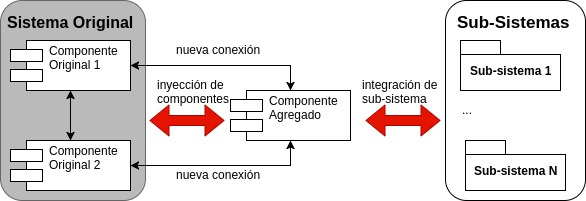
\includegraphics[width=5 in,totalheight=3 in] {Ch0/EstructuraSolucion}
 % .: 0x0 pixel, 0dpi, 0.00x0.00 cm, bb=
\caption{Estructura de la solución} \label{fig:solucion}
\end{center}
\end{figure}

La parte gris de la figura representa las componentes de un sistema original
con sus componentes y relaciones. Luego se representa el agregado de una nueva
componente (\textit{componente agregada}) que se relaciona con las
\textit{componentes originales} del sistema por medio de \textit{nuevas
conexiones}. Esta nueva relación se denomina \textit{inyección de componentes}.
Luego la \textit{componente agregada} se conecta con diferentes subsistemas. De
esta manera queda conformado un nuevo sistema a partir del
original, proponiéndose una ''estructura de la solución para
el DHD” (EstDHD).

En este caso, la componente agregada es el comienzo de la
construcción de un modelo de contrato orientado a la implementación de servicios
sensibles al contexto. El uso de contratos parte de la noción de Programación
por Contrato (”Programing by Contract”) de Meyer \cite{cap1.11} basada en la
metáfora de que un elemento de un sistema de software colabora con otro,
manteniendo obligaciones y beneficios mutuos. En el dominio de aplicación cabe
considerar que un objeto cliente y un objeto servidor “acuerdan“,  mediante el uso de 
un contrato (representado con un nuevo objeto) que el objeto servidor satisfaga
el pedido del cliente y, al mismo tiempo, que el cliente cumpla con las condiciones
impuestas por el proveedor.

Como ejemplo de la aplicación de la idea de Meyer en un dominio de
sistema colaborativo e-learning se expone la situación en que un
usuario (cliente) utiliza un servicio de edición de mensajes (servidor) a través
de un contrato que garantizará las siguientes condiciones: el usuario debe poder
editar aquellos mensajes que tienen autorización según su perfil (obligación del
proveedor y beneficio del cliente); y el proveedor debe tener acceso a la
información del perfil del usuario (obligación del cliente y beneficio del
proveedor).

A partir de la conceptualización de contratos según Meyer, se propone una
extensión por medio del agregado de nuevas componentes para instrumentar
mecanismos que permitan ejecutar acciones dependiendo del contexto (figura
\ref{fig:solucion}).

En aplicaciones sensibles al contexto \cite{cap1.6}, el contexto, o información
de contexto, es definido como la información que puede ser usada
para caracterizar la situación de una entidad más allá de los atributos que la
definen. En un caso del campo educativo, una entidad es un usuario (alumno, docente, autoridad de la institución),
lugar (aula, biblioteca, sala de consulta, etcétera), recurso (impresora, fax, etcétera),
u objeto (examen, trabajo práctico, etcétera) que se comunica con otra entidad a
través del contrato. En \cite{cap1.2} se propone una especificación del concepto
de contexto partiendo de las consideraciones de Dourish \cite{cap1.20} y
adaptadas al dominio de sistemas colaborativos con funcionalidades e-learning,
que se consideran en este trabajo.
Contexto es todo tipo de información que pueda ser censada y procesada, a través
de la aplicación (por ejemplo, una aplicación colaborativa e-learning), que
caracterizan a un usuario o entorno, por
ejemplo: intervenciones en los foros, promedios de notas, habilidades, niveles
de conocimientos, máquinas (direcciones IP) conectadas, nivel de intervención en
los foros, cantidad de usuarios conectados, fechas y horarios, estadísticas
sobre cursos, etcétera.

En términos generales, la coordinación de contratos es una conexión establecida entre un grupo de objetos, aunque, debe recordarse que según los objetivos de esta investigación sólo se consideran dos objetos: un cliente y un servidor.

Cuando un objeto cliente efectúa una llamada a un objeto servidor (ej., el
servicio de edición de la herramienta Foro), el contrato ”intercepta” la
llamada y establece una nueva relación teniendo en cuenta el contexto del
objeto cliente, el del objeto servidor y la información relevante adquirida
y representada como contexto del entorno [20]. Como condición necesaria, el uso
de contratos no debe alterar la funcionalidad de la implementación de los
objetos participantes, aunque sí se espera que altere la funcionalidad del
sistema.

A continuación, se presenta sintéticamente un modelo conceptual de contratos sensibles
al contexto de donde se infieren las distintas soluciones propuestas en esta
tesis. Se brindarán detalles sobre algunos de los componentes y relaciones
esenciales para la integración de este modelo con el framework colaborativo que
se identifica con la parte gris de la figura \ref{fig:solucion} y algunos de
sus sub-sistemas representados.


\subsection{Primera noción de los elementos intervinientes en la solución}
\label{sec:elementoscontrato}

Un contrato que siga las ideas de Meyer contiene toda la información
sobre los servicios que utilizarán los clientes. Para incorporar sensibilidad
al contexto los contratos deberán tener referencias sobre algún tipo de
información de contexto que posibilite su utilización.

En el diagrama de relaciones entre entidades analizado en la Figura
\ref{fig:contratosv1} se presenta una primera descripción de los elementos
que componen el concepto de contrato sensible al contexto. A lo largo de la
tesis este mismo diagrama será utilizado para describir diferentes aspectos de
una misma solución. 


\begin{figure}[h]
\begin{center}
 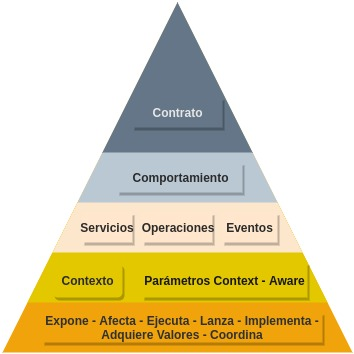
\includegraphics[width=3.5 in,totalheight=3 in] {Ch0/PiramideDHD}
 % .: 0x0 pixel, 0dpi, 0.00x0.00 cm, bb=
\caption{PirámideDHD: Primera interpretación de contratos}
\label{fig:contratosv1}
\end{center}
\end{figure}


La configuración de este diagrama se centra en las etapas de diseño e
implementación de diferentes modelos de integración con sub-sistemas
(capítulos \ref{cap:5}, \ref{cap:6},  \ref{cap:7}). 


En la figura también se muestran los elementos tenidos en cuenta
para la instrumentación de la noción de contrato. Cada uno de los bloques
apilados (desde el pilar 1 al pilar 5) en forma de piramidal pueden representar
componentes abstractas o concretas. En el bloque base se encuentran las
relaciones que intervienen entre las componentes superiores (pilar 1). Luego
aparecen los bloques de contexto y parámetros context-aware (pilar 2), que
permitirán configurar relaciones que posibilitan resolver requerimientos de
adaptación. Seguidamente, se encuentran los bloques que identifican componentes concretos que
integran las herramientas colaborativas (pilar 3) que están sujetas a
modificaciones para establecer las relaciones del bloque base para que se incorporen los
elementos intermedios (pilar 2). Los últimos dos pilares tienen que ver con el
comportamiento (pilar 4) que implementan los pilares inferiores, el contrato
(pilar 5) representa la pieza de software que permitirá el control externo. 

A continuación, se presenta la descripción individual de los componentes más importantes:

\textbf{Servicios}: En este componente se representan los elementos necesarios
para la identificación de un servicio y clasificación de los servicios que
pueden formar parte de las acciones de los contratos. Por ejemplo, nombre del
servicio, identificadores, alcance, propósito, etc. Para más detalles
consultar \cite{cap1.5}. El comportamiento funcional de cada servicio se
expone a través de la componente Comportamiento.

\textbf{Comportamiento}: El comportamiento de un servicio se logra a partir de
combinar operaciones y eventos que son representados por las componentes
Operaciones y Eventos. 

\textbf{Parámetros Context-Aware}: Se denomina parámetros context-aware a la
representación de la información de contexto que forma parte de los
parámetros de entrada de las funciones y métodos exportados por los servicios,
estableciendo de esta manera una relación entre el componente “Servicios” y el
componente “Parámetros” context-aware. La influencia de estos parámetros en el
comportamiento funcional de los servicios es representada a través de
la relación entre los componentes “Parámetros” context-aware y “Comportamiento”.

\textbf{Contexto}: Este componente representa el contexto o información de
contexto , que fue definido en páginas anteriores. Para el modelo planteado en esta tesis, este tipo
de información es utilizada de dos maneras diferentes: 1. para la
asignación de los valores que toman los “Parámetros” context-aware; 2. esta información puede ser utilizada para definir los invariantes que se
representan en los contratos.

Otro de los elementos importantes que se tendrán en cuenta para la
propuesta de solución es el tipo de representación que se
determina para el entorno. Para este propósito se observará que ligado al
entorno se provea una infraestructura que permita distribuir el contexto
producido por las fuentes. Esta infraestructura fue denominada capa de contexto,
y sirve de intermediaria entre las fuentes contextuales y los elementos que
permitirán inyectar las propiedades de sensibilidad al contexto del DHD.


\section{Limitaciones}	


\section{Organización del documento}

\begin{description}
 \item[Capítulo 1:]
 \item[Capítulo 2:]
 \item[Capítulo 3:]
 \item[Capítulo 4:]
 \item[Capítulo 5:]
 \item[Capítulo 6:]
 \item[Capítulo 7:]
 \item[Capítulo 8:]
 \item[Apéndice:]
 \item[Bibliografía:]
\end{description}




% -- Archivo Cap\'{\i}tulo N� 1 --
%%-------	-------------------------------------------------------------------------------------------
%------------------------------------------------- Chapter --------------------------------------------------------
\chapter{Estado del Arte} \label{cap:estadodelarte} \label{cap:3}
%\pagenumbering{arabic} 


\section{Introducción}

Este capítulo presentará el estudio del estado del arte, partiendo de
la transformación de \textit{información de contexto} como componente de primera clase y visible en una arquitectura \ref{cap:arqdhd}, tratado a través de un sistema especializado para su uso. En este sentido, se desarrollarán las principales características de los sistemas y las estructuras que fueron utilizadas para la construcción de una propuesta de solución que determina un modelo evolutivo. También, aparecerá  otro elemento de primera clase integrado a un sistema que permite su manejo brindando conexión con los anteriores. Así, esta combinación de elementos y sistemas configuran una
estructura de evolución que sustenta parte de la arquitectura del DHD.




\section{Contexto en el DHD}

En el capítulo \ref{cap:introduccion} se referenció al contexto en
virtud de las propiedades de sistemas especializados en usar información
de contexto para brindar funcionalidades. Además, el contexto aparece como uno
de los elementos, junto a los parámetros context-aware, que forma la
pirámide de componentes de la solución propuesta (figura \ref{fig:contratosv1}).
Luego, en el capítulo \ref{cap:dhd} el contexto forma parte de la definición
conceptual del DHD como un factor a tener en cuenta para la adaptación debido a
su influencia en los \hyperref[requerimientosdhd]{RequerimientosDHD}
(\hyperref[ejemplo1]{véase ejemplos}). 

En el presente capítulo, se abordará la caracterización del contexto teniendo en cuenta la taxonomía diseñada en el DHD. Esta forma de representación posibilita describir al contexto a través de una interpretación necesaria para su tratamiento tecnológico.


\subsection {Caracterización del Contexto}

En esta tesis se referencia al contexto para cada una de las representaciones considerando tanto los diferentes diseños para modelarlos según su tipo dependiendo de las necesidades, como su transformación en información (información de contexto)  para las interfaces de los mecanismos de los sistemas y/o subsistemas sensibles al contexto.

\subsubsection{Origen del contexto en el DHD}

En la figura \ref{fig:ontologiaContexto} se representan los orígenes de la conformación del contexto en el DHD. Las componentes grises son precisamente las diferentes fuentes donde se obtiene información de contexto. Por otro lado, las demás componentes de color blanco tienen una influencia en los procesos de su construcción. 

Existen diferentes categorías de contexto en relación a características de tipología dinámica o estática. En este sentido, los \textit{roles} y \textit{permisos} asociados a los diferentes tipos de usuarios (\textit{Miembros en formación} y \textit{Grupo Responsables}) ayudan a
caracterizar parte del perfil de un usuario. Esto permitirá ajustar determinados tipos de acciones para las diferentes herramientas (wiki, foro, videoconferencias, etc). Los servicios (ej.: agregar, borrar, etc.) que se consideran partes de las herramientas, deberán ser sensibles a la influencia del entorno teniendo en cuenta la información sintetizada que de este deviene. En este caso, en el entorno del DHD está caracterizada por información que se puede representar a trav´es de los siguientes elementos: 


\begin{figure} 
\begin{center}
 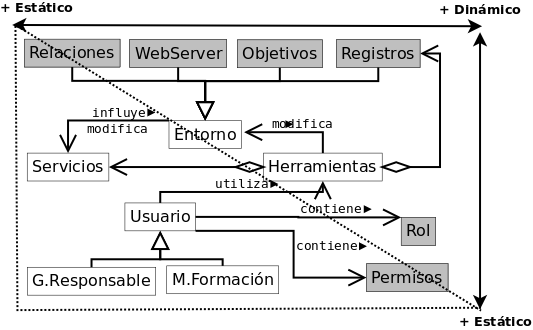
\includegraphics [width=5 in,totalheight=3 in] {Ch1/Figuras/contexto.png}
 % .: 0x0 pixel, -2147483648dpi, nanxnan cm, bb=
\caption {Fuentes del contexto del DHD}
\label{fig:ontologiaContexto}
\end{center}
\end{figure}



\begin{itemize}
 \item WebServer: información que se obtiene a partir de los \textit{logs}
del
servidor Web que permite la ejecución de las aplicación web colaborativas del
DHD. También es utilizada información de la configuración  sobre el modo
de ejecución, puertos habilitados, librerías, componentes, aplicaciones
instaladas, políticas de seguridad, tipos de sesiones, manejo y notificación
de errores, tipos de conexiones, etc.

\item Objetivos: información relacionada a los objetivos que se persiguen a
partir de ciertas configuraciones de los ambientes colaborativos del DHD. Estos
objetivos deben estar relacionados con los
\hyperref[requisitosdhd]{RequisitosDHD}
y/o \hyperref[requerimientosdhd]{RequerimientosDHD}
en los que se encuentran involucrados Stakeholder \footnote{Stakeholder es un
término inglés utilizado por primera vez por R. E. Freeman en su obra:
“Strategic Management: A Stakeholder Approach”, (Pitman, 1984) para referirse a
«quienes pueden afectar o son afectados por las actividades de una empresa».} de
forma directa o indirecta. 

\item Registros: información generada a partir de las diferentes
intervenciones de los usuarios con las herramientas que componen un espacio
colaborativo \footnote{El espacio colaborativo (Collaborative Learning) es
un conjunto de métodos de instrucción y entrenamiento apoyados con tecnología
así como estrategias para propiciar el desarrollo de habilidades mixtas
(aprendizaje y desarrollo personal y social) donde cada miembro del grupo es
responsable tanto de su aprendizaje como del de sus compañeros.}.
Habitualmente esta información aparece en forma de tablas donde se
almacena, entre otras, identificador de usuario, tiempo, la herramienta y
el servicio utilizado.

\item Relaciones: información que permite interpretar
\hyperref[interactividadDHD]{interactividades DHD} a través de la
descripción de eventos secuenciados que indican relaciones entre usuarios,
herramientas, servicios, información de contexto, sitios y otros tipo de
información tecnológica comunicacional.

\item Rol: información asociada con los usuarios de los sitios que definen
deferentes perfiles de usuarios para establecer el rol que cumplen en los procesos
colaborativos. Como ejemplo de los tipos de roles se pueden mencionar a los
``Miembros en formación``, ''Grupos Responsables``, ``Administradores'', etc
\cite{libro}.

\item Permisos: se relaciona al tipo de accesibilidad que un usuario tiene
en las herramientas de los distintos espacios colaborativos. Particularmente en
Sakai los permisos están directamente asociados con los roles. En la figura
\ref{fig:rolesSakai,fig:rolesSakai2} se muestra un ejemplo tomado de la propia
interfaz Sakai
donde se visualizan las relaciones entre un identificador de usuario y roles. 
Los permisos que permiten ejecutar las operaciones: \textit{ver},
\textit{editar}, \textit{borrar} y demás manipulación de datos asociados a las
herramientas Sakai, se manejan por medio del uso de \textit{realms}
\cite{sakaimanual}. Cada \textit{realm} tiene uno a más roles para asignar a los
usuarios. Los permisos son administrados a
través de la herramienta \textit{Realms}
\footnote{La herramienta Realms de Sakai es utilizada en la administración de
permisos y roles para cada uno de los sitios.}. Se expone un ejemplo de la
estructura de \textit{permisos}, \textit{roles}, \textit{tipo} y
\textit{dominios}, que se implementan en una
plataforma colaborativa Web. El anexo \ref{anexo_permisos} contiene
información ampliada sobre las posibilidades de configuraciones de Sakai. A
continuación se muestra un pequeño resumen para ejemplificar lo expuesto.
Véase en \cite{permisos_roles} una descripción completa. 


\begin{figure} 
\begin{center}
 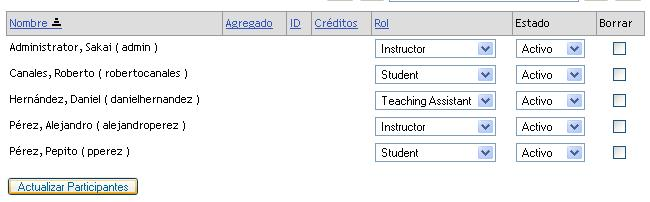
\includegraphics [width=4 in,totalheight=2 in] {Ch1/Figuras/RolesSakai.jpg}
 % .: 0x0 pixel, -2147483648dpi, nanxnan cm, bb=
\caption {Una de las interfaces para la asignaciones de roles Sakai}
\label{fig:rolesSakai}
\end{center}
\end{figure}


\begin{figure} 
\begin{center}
 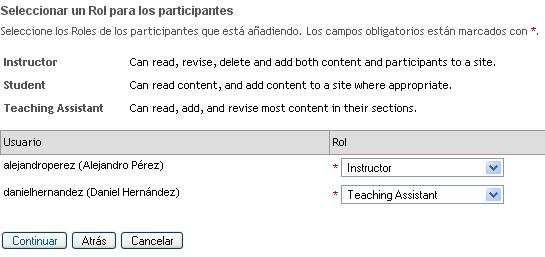
\includegraphics [width=4 in,totalheight=2 in] {Ch1/Figuras/RolesSakai2.jpg}
 % .: 0x0 pixel, -2147483648dpi, nanxnan cm, bb=
\caption {Una de las interfaces para la asignaciones de roles Sakai}
\label{fig:rolesSakai2}
\end{center}
\end{figure}



\begin{itemize}
 \item Un \textit{realm} define los permisos de ciertos objetos de la aplicación

\begin{itemize}
\item Contienen varios roles
\item Cada rol contiene los unos determinados permisos
\item Contiene los usuarios asignados al \textit{realm} y con que rol está
asignado
\item Cada \textit{realm} indica que rol es el de mantenimiento
\item Los \textit{realms} se editan con la herramienta de ‘Edición de Realms’
\item Permite crear nuevos roles
\item Permite editar los permisos de los roles
\item Permite incluir usuarios
\end{itemize}

\begin{itemize}
 \item Los \textit{realms} se editan con la herramienta de ‘Edición de Realms’

\begin{itemize}
\item Permite crear nuevos roles
\item Permite editar los permisos de los roles
\item Permite incluir usuarios
\end{itemize}


\item Los roles por defecto de Sakai

\begin{itemize}
\item $!$site.template \rightsquigarrow  \textit{access}, \textit{maintain}

\item $!$site.template.course \rightsquigarrow \textit{Instructor},
\textit{Student}, \textit{Teaching}, \textit{Assistant}
\end{itemize}

\item Role del creador del Site

\begin{itemize}
 \item Por defecto \textit{maintain}, \textit{Instructor}
\item Está especificado por el campo mantenedor del \textit{realm}
\end{itemize}


\end{itemize}
\end{itemize}
\end{itemize}



%\subsubsection{Contexto versus información del contexto}
%\label{sec:informacionContexto}
%En la figura \ref{fig:ontologiaContexto} 


\subsubsection {Modelado del contexto} \label{sec:contextodhd}

En esta sección se muestran
algunos resultados en base al actual estado del arte que servirán como referentes
descriptivos sobre el tipo de modelo de contexto que mejor se adaptaría a las
necesidades del DHD. En este  sentido, se presenta una referencia a un metamodelo creado para un
lenguaje de desarrollo de software guiado por modelos para servicios Web
sensibles al contexto basado en UML\cite{ContextUML} 

\subsubsection{ContextoDHD: Contexto para los servicios DHD}\label{contextodhd}

Un \textit{servicioDHD}\label{serviciodhd} es un servicio con sensibilidad al
contexto que puede tener cierta flexibilidad para resolver 
\hyperref[RequerimientosDHD]{Requerimientos DHD}. Esto significa que dichos
servicios estarán orientados al tipo de tarea que desempeña un usuario bajo
un determinado contexto. 


Debido a la heterogeneidad de la información de contexto suministrada,
imperfecciones en la transformación de datos, información redundante, malas
interpretaciones sobres funcionalidades \hyperref[no_computable]{no
computables} y la información dinámica del entorno; es imprescindible tener
una representación adecuada\cite{contextToolKit}. En particular, varios
proveedores de contexto pueden estar reportando las mismas piezas de contexto
pero con distintas representaciones. Esto dificulta su especificación en
las etapas de diseño. 

En los capítulos anteriores se expusieron fundamentos sobre la
importancia del contexto en el DHD y consideraciones sobre su visualización funcional a través de formas computables de representación. Por este motivo, en esta sección se presentan aspectos de
diseño sobre el estado del arte del modelado de contexto que mejor se adapta
para las representaciones en el DHD. 


En la figura \ref{fig:contextMetamodel} se muestra una adaptación del
metamodelo creado para ContextUML\cite{contextUML} que fundamenta la
creación de una sintaxis abstracta de un lenguaje considerando dos
aspectos:
\textit{modelado del contexto} y \textit{modelado de los mecanismos
de sensibilidad del contexto} (o en inglés context awareness).


\begin{figure} 
\begin{center}
 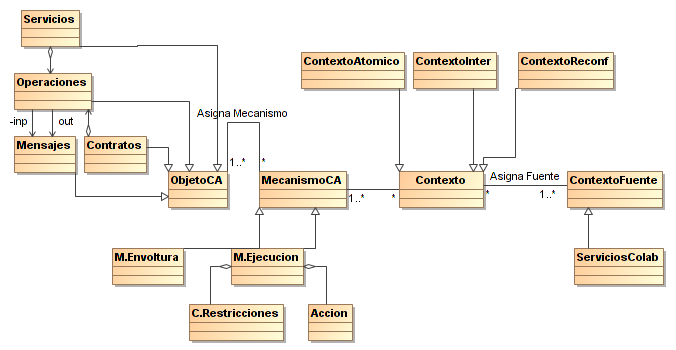
\includegraphics [width=5 in,totalheight=3 in]
{Ch1/Figuras/ContextoDHD}
 % .: 0x0 pixel, -2147483648dpi, nanxnan cm, bb=
\caption {Metamodelo del contexto para el DHD}
\label{fig:contextMetamodel}
\end{center}
\end{figure}



\textit{Contexto} es la clase que modela la información de contexto. En nuestro
diseño adaptado, el tipo de contexto está extendido en dos categorías
diferentes como subtipos \textit{CotextoInter}, \textit{ContextoReconf} y
\textit{ContextoAtomico}. El contexto atómico es información con el menor
nivel de abstracción posible y no comparte relación con otra porción de
contexto. Por otra lado, el contexto de las interacciones tiene que ver con
información de contexto que colabora en la descripción de las 
\hyperref[intersubjetivas]{relaciones intersubjetivas}. De la misma manera, el
contexto para la reconfiguración es una abstracción de los parámetros
\textit{context-aware} enunciados en \ref{sec:elementoscontrato}. Estos tres
subtipos agrupan a las fuentes del contexto descripto en la figura
\ref{fig:ontologiaContexto}, con lo cúal ya se cuenta con tres niveles de
caracterización del contexto para el DHD. De esta manera, se continúa con similares lineamientos utilizados en el DHD para lograr una representación
acorde del contexto hacia su implementación tecnológica. 


Es claro observar que desde los servicios se encapsula (oculta) la forma de
adquirir el contexto. Así, en las implementaciones
donde intervienen servicios de herramientas se usará su misma
representación, accediendo a esta información a través de los accesos
tecnológicos de la implementación. Por ejemplo, acceso a la bases de datos,
acceso a información del servidor Web o del ambiente contenedor de los
lenguajes intervinientes (ej., Apache Tomcat \footnote{Tomcat es un servidor web
con soporte de Servlets y JSPs. Incluye el compilador Jasper, que compila JSPs
convirtiéndolas en
Servlets. El motor de Servlets de Tomcat a menudo se presenta en combinación con
el servidor web Apache.}). En otras palabras, se puede decir que el concepto de
contexto del servicio oculta la complejidad de su adquisición
bajo la perspectiva de los Sistemas Sensibles al Contexto \ref{sec:cas} (o
también mencionados como Sistemas Context-Aware).



\paragraph{Fuentes de la información de contexto}

El tipo de contexto fuente (\textit{ContextoFuente}) caracteriza desde donde
parte la construcción del
contexto que luego será almacenada para su recolección, por ejemplo, en el
registro de actividades. Uno de los subtipos de fuentes pueden ser los
servicios colaborativos (representado por \textit{ServiciosColab}) que son
utilizados en los servicios de las herramientas colaborativas (ej., Wiki, Foro,
etc.).
En este caso se tiene una alta dependencia de la implementación de los
framework originales (e.i., sin la inyección de contratos sensibles al
contexto). 

Es observable que desde los servicios se encapsula (oculta) la forma de
adquirir el contexto. De esta manera, en las implementaciones
donde intervienen servicios de herramientas, se usará su misma
representación, accediendo a esta información a través de los accesos
tecnológicos de la implementación. Por ejemplo, acceso a la bases de datos,
acceso a información del servidor Web o del ambiente contenedor del los
lenguajes intervinientes (ej., Apache Tomcat \footnote{Tomcat es un servidor web
con soporte de servlets y JSPs. Tomcat no es un servidor de aplicaciones, como
JBoss o JOnAS. Incluye el compilador Jasper, que compila JSPs convirtiéndolas en
servlets. El motor de servlets de Tomcat a menudo se presenta en combinación con
el servidor web Apache.}). En otras palabras, se puede decir que el concepto de
contexto del servicio oculta la complejidad de de la adquisición del contexto,
bajo la perspectiva de los Sistemas Sensibles al Contexto \ref{sec:cas} (o en
inglés Context Aware System).



\paragraph{Contexto para los servicios de reconfiguración}

El subtipo representado por la clase \textit{ServicioReconf} interpreta a todos
los servicios que devienen de las reglas implementadas por los contratos, mas
precisamente, están relacionados con las acciones de estas reglas
\ref{cap:contratos}. Por otro lado, los condicionales que forman parte de las
mismas reglas se vinculan con la clase \textit{Contexto} haciendo las veces de
pre-condición; mientras que los resultados de las acciones
establecerán  post-condiciones. De esta manera se fundamenta uno de los
elementos sobre el por qué de la elección de los contratos como
pieza de software base para implementar la reconfiguración y promover la
dinámica del DHD.  



\paragraph{Modelado de la sensibilidad del contexto}

\textit{MecanismoCA} es la clase que centraliza la formalización de los
mecanismos que permiten el modelado para su implementación de las propiedades
de sensibilidad al contexto. Para este propósito se han definido dos
diferentes categorías por medio de los subtipos \textit{M.Envoltura} y
\textit{M.Ejecuciones }. Este mecanismo permitirá determinar la asociación de
la información de contexto  con objetos concretos que brindan funcionalidades
en el sistema. Estos objetos son representados por la clase \textit{ObjetosCA}.
Hay 5 subtipos de \textit{ObjetosCA}: Servicios, Operaciones, Mensajes, Partes y
Contratos. Cada servicio ofrece varias operaciones y cada operación pertenece
a un sólo servicio. Este vínculo se representa por una relación de
agregación. Cada operación tendrá un mensaje de entrada y/o uno de salida
con la posibilidad de que esos mensajes tengan partes particulares (i.e.,
mensajes con parámetros). La otra posibilidad es que en vez de mensajes se
utilicen, con el mismo propósito, contratos para establecer igual tarea de
comunicación con el agregado de mayores propiedades semánticas.
Para este caso se estable una nueva relación de agregación entre
\textit{Operaciones} y \textit{Contratos}.



\subparagraph{Mecanismos de Envolturas}
El subtipo de \textit{M.Envolturas} modela los procesos automáticos de envoltura
o vinculación de la información de contexto para que pueda ser procesada por
los mecanismos de sensibilidad al contexto. Por ejemplo, en el caso que una
operación tome como parámetro un conjunto de caracteres (``string``) para
identificar un \textit{tema} de un foro, supongamos que un usuario tiene
intervenciones en dicho tema del foro con información de contexto referente a su
rol (ej., ''perteneciente al grupo responsable``). Entonces, el mecanismo
envoltura debe vincular el parámetro \textit{tema} con el \textit{rol grupo
responsable}.

Una vinculación automática de contexto (e.i., una envoltura de contexto) es
una asignación (''mapping'') entre un contexto y un objeto sensible al
contexto (ej., un parámetro de entrada de una operación de servicio). La
semántica se refiere a que un valor del objeto es reemplazado por un valor de contexto.
Cabe aclarar que el valor de un objeto sensible al contexto puede derivar varios
valores de contexto. 
 

\subparagraph{Mecanismos de Ejecución}

El subtipo \textit{M.Ejecución} modela la situación de la adaptación de
contexto
donde los servicios pueden ser ejecutados o modificados según la información
de contexto. Un contexto del mecanismo de ejecución contiene dos partes: un
conjunto de restricciones de contexto (\textit{C.Restricciones}) y un
conjunto de acciones (\textit{Acciones}), donde la semántica de esas acciones
pueden ser ejecutadas si
y sólo si se cumplen todas las restricciones impuestas para el contexto. 

Las restricciones de contexto especifican que ciertos contextos deben reunir
determinadas condiciones con el propósito de cumplir ciertas operaciones.
Formalmente, una restricción para el contexto puede estar modelada como un
predicado\cite{ContextUML} (i.e, una expresión booleana) que consiste en un
operador y dos o más operando. En los lugares donde interviene el contrato
estas expresiones podrán ser representadas como parte de los condicionales
de las reglas. En el caso que esto no ocurra, \textit{M.Ejecución} será el
encargado de implementar las restricciones. Un ejemplo de estas expresiones
puede ser: 

\begin{verse}

\begin{verbatim}
tema_foro='\%DHD\%' and id_foro=1233
\end{verbatim}               

\end{verse} 


para indicar que el operador se ejecutará si se
está en un Foro, identificado con el número “1233”, donde el tema tenga el
string “DHD”. Esta forma de interpretación posibilita además poner en
la misma expresión de acciones para el caso que no se cumpla la condición.

Existe un lenguaje para ContextUML\cite{ContextUML} que puede ser usado para
este mismo modelo de contexto en la programación de acciones desde
el propio mecanismo que implementa la sensibilidad al contexto. En esta tesis,
es de interés utilizar solamente el modelo de contexto y todas las acciones de
adaptabilidad serán mediadas por la componente contrato. 




\section{Sistemas Sensibles al Contexto} \label{sec:cas}


En esta sección se toma el antecedente de la representación y
formas de utilización del contexto, información de contexto, mecanismos de
manipulación y las fuentes de recolección en el DHD. El propósito, es
interpretar la posibilidad de agregar a un sistema
colaborativo Web (original) las propiedades de sensibilidad del
contexto creadas para el DHD (ContextoDHD).

Podemos entender a un sistema colaborativo sensible al
\hyperref[contextodhd]{contextoDHD} como una
aplicación provista de mecanismos que permiten una mejor adaptación de los
servicios, a partir del contexto de los usuarios y del entorno. En ambientes
colaborativos para educación, los servicios forman parte de las funcionalidades
observables, desde las perspectivas de los usuarios (ej.: alumno, docente, etc.),
que proveen las herramientas del dispositivo (ej., wiki, foros, mensajería,
glosario, recursos, etc.). Los elementos que componen la caracterización del
contexto deben pertenecer a un dominio bien definido, manteniendo ciertos
niveles de concordancia con los mecanismos encargados de manipularlos y la toma
de decisiones en base a ellos.

A través de un simple diagrama, es posible observar algunas de las características
fundamentales que determinan un sistema colaborativo sensibles al contexto,
donde se
encuentran remarcadas aquellas particularidades (tecnológicas y
conceptuales) que se vinculan con la perspectiva del DHD. En la figura
\ref{fig:evolucion}, describimos desde una arquitectura básica y genérica, tres
tipos de niveles, cada uno agrega nuevos rasgos y comportamientos que
condicionan los servicios del dispositivo hipermedial hacia un nuevo modelo.

\begin{figure}
\begin{center}
 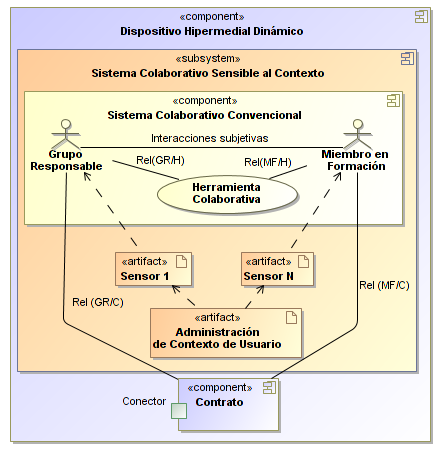
\includegraphics[width=3.5 in,totalheight=3.5in] {Ch1/MEvolutivo.png}
 % .: 0x0 pixel, 0dpi, 0.00x0.00 cm, bb=
\caption{Arquitectura propuesta evolutiva.}\label{fig:evolucion}
\end{center}
\end{figure}

La figura está dividida en tres bloques fundamentales, en el primero (Sistema
Colaborativos Web Convencional) se describen los principales componentes y
relaciones; fundamentalmente un alumno puede interactuar con las herramientas y
servicios del sistema y comunicarse con un docente o con sus pares.


El segundo bloque de la figura (Sistema Colaborativo Sensible al
Contexto) contiene el
agregado de dos componentes esenciales, sensores y un administrador de contexto.
Los
sensores capturan información del usuario y del entorno, son partes
fundamentales para
la recolección de información; si los sensores juegan un papel secundario, los
podemos
enmarcar bajo el concepto de artefactos virtuales. El segundo componente hace
referencia a la administración del contexto, donde se destacan las siguientes
funcionalidades: recolección, abstracción, interpretación, comunicación y
almacenamiento. Para la implementación de comportamientos context-aware los
diseños de software deben completarse con diferentes modelos, para el caso de
los
denominados sistemas e-learning, las soluciones se focalizan en la tecnología de
comunicación e información que utilizan los usuarios. MatchBase (Gross et al.,
2006)
es un proyecto de referencia en cuanto al uso de estos tipos de diseño y
tecnología,
conformando una herramienta para el desarrollo de comunicaciones contex-aware.
Fue
trasladado como experiencia a proyectos de investigación de sistemas e-learning
context-aware (Schmidt, 2005). Pensar en aplicaciones para educación e
investigación sensibles al contexto dentro del marco teórico context-awareness
conforma un nuevo paradigma, donde las relaciones (rotuladas con “Rel
(fuente/destino)” en la figura) cobran un mayor protagonismo en la concepción de
los marcos conceptuales propuestos como soluciones a nuevos requerimientos
académicos para el contexto físico-virtual.


Perspectivas como la del DHD, también centran los requerimientos sobre
las relaciones y comunicaciones entre los principales componentes del
dispositivo,
focalizados en las relaciones entre los actores (Recursos Humanos en formación,
grupos
responsables) y los servicios brindados por las herramientas anteriormente
mencionadas, a las que se les integra el potencial de comunicación hipermedial
como
por ejemplo, video conferencias, edición en variados formatos, etc.

Retomando la evolución de los sistemas colaborativos referida a la adaptación de
modelos
para requerimientos educativos complejos, el último bloque de la figura
(Dispositivos
hipermediales sensibles al ContextoDHD Dinámico) representa un modo de
interpretación de una
nueva configuración de la arquitectura de un sistema, debido a la interposición
de la
componente contratos (referenciada con el dibujo característico para componentes
de
software en UML). Al agregar este nuevo elemento que permite una mejor
articulación
de las relaciones, resulta una nueva teoría que proporciona conceptualmente un
marco
innovador para las prácticas de diseño, desarrollo, uso de dispositivos y
aplicaciones en dicho campo.


El contrato debe ser visto como una alternativa de abstracción de las relaciones
mencionadas anteriormente, determina un nuevo tipo de relación que mantiene las
características de los anteriores bloques de la figura y además, reduce la
complejidad de
los modelos de los SSC en la adaptación de los servicios que interfieren
en
relacionamientos entre usuarios y comunicacionales. Los contratos se nutren con
información del contexto por medio de sus parámetros; no intervienen en la
recolección,
ni en la abstracción, ni en la distribución del contexto y en principio pueden
ser
adaptados a cualquier modelo de sensibilidad al contexto similar, bajo la
perspectiva propuesta por Dey. et. al (2001).


A continuación, se analizan las principales características de los
SSC.
Como observamos en la figura anterior, el bloque intermedio se configura como
articulador entre los sistemas colaborativo tradicionales y las
nuevas posibilidades
tecnológicas que permiten la concreción más efectiva del Dispositivo
Hipermedial
Dinámico agregando la componente Contrato.

Esta propuesta evolutiva y la forma de representación del contexto mantiene
los principios que definen la teoría de los SCC.

El contexto puede definirse de manera general como:

\begin{quote}
Cualquier información que puede usarse para caracterizar la situación de
una entidad. Donde una entidad es una persona, lugar u objeto que es
considerado relevante para la interacción entre un usuario y una
aplicación, incluyendo al usuario mismo y la aplicación
\begin{flushright}(Dey y Abowd, 2000)\end{flushright}
\end{quote}  


Las aplicaciones sensibles al contexto se definen  como:


\begin{quote}
Aquellas que usan el contexto para proveer información y/o servicios
relevantes al usuario, donde la relevancia depende de la tarea del usuario.
\begin{flushright}(Dey y Abowd, 2000)\end{flushright}
\end{quote}

Según un análisis realizado por Brown et al., (2000), entre las aplicaciones
sensibles al contexto, la recuperación de información juega un papel
central, y
tales aplicaciones parecen confirmarse como la prospectiva que requiere el
computo consiente de contexto.

Por lo tanto, en las aportaciones de los autores de los trabajos que
presentaremos a
continuación, tomaremos el problema planteado en el marco de la recuperación de
información consiente de contexto.

\subsection {Propuestas para la Identificación del Contexto} 

Algunos trabajos se han enfocado sobre cómo identificar el contexto
efectivamente y
cómo obtener una representación del mismo que pueda ser utilizada para
incorporarlo a
la búsqueda de información relevante para el usuario.

Budzik y Hammond, (2000) clasifican los esfuerzos llevados a cabo para esta
tarea en cuatro categorías:

\begin{itemize}
\item \textbf{Retroalimentación sobre la relevancia de los resultados}: Trata
de determinar el contexto obteniendo cierta retroalimentación por parte del
usuario respecto al nivel
de relevancia de los resultados que pueda tener una consulta (Salton y
Buckley, 1990).


\item \textbf{Perfiles de usuario}: en este caso los intereses del usuario se
integran para formar un
perfil que es efectivo a lo largo de varias consultas, un ejemplo de este
enfoque es
Letizia (Lieberman, 1995).

\item \textbf{Eliminación de ambigüedad en el sentido de las palabras}: Algunos
sistemas tratan
de eliminar posibles ambigüedades pidiendo al usuario que lo haga explícitamente
(Cheng y Wilensky, 1997), mientras que otros, lo hacen implícitamente usando la
popularidad de los términos según la estructura interna de los documentos de
hipertexto (Bradshaw y Hammond, 1999).

\item \textbf{Enfoques de ingeniería del conocimiento}: intentan crear un modelo
de
comportamiento del usuario mientras estos se encuentran interactuando con una
aplicación.
\end{itemize}

A su vez, Lawrence (2000) propone cinco tipos de estrategias para incluir el
contexto en
las búsquedas:

\begin{itemize}

\item \textbf{Agregar información de contexto en forma explicita}: se presentan
al usuario
mecanismos para que éste especifique el contexto en el cual desea realizar su
búsqueda. Tal es el caso del proyecto Inquirus 2 (Glover et al., 2000).

\item \textbf{Inferir la información de contexto automáticamente}: los sistemas
tratan de obtener
dicha información de contexto sin la intervención conciente del usuario,
usualmente
monitoreando las actividades y aplicaciones de éste. El proyecto Watson (Budzik
y
Hammond, 2000) se inscribe en esta categoría. Siguiendo este mismo enfoque hay
sistemas que recomiendan enlaces a sitios Web dinámicamente mientras el usuario
realiza sus tareas, algunos ejemplos de este tipo de sistemas son: The
Remembrance
Agent (Rhodes, 2000), SurfLen (Fu et al., 2000), Margin Notes (Rhodes, 2000), y
Fab (Balabanovic, 1997).

\item \textbf{Búsquedas personalizadas}: este concepto implica que una máquina
de búsqueda
conozca todas las búsquedas anteriores del usuario y que use esa información
para
personalizar los resultados de búsquedas futuras. Con el buscador Northern Light
el
usuario recibe notificaciones sobre nuevas páginas que concuerden con ciertas
expresiones de búsqueda.

\item \textbf{“Adivinar” lo que el usuario quiere}: este enfoque consiste en
examinar la expresión
de búsqueda del usuario y cuando se encuentran ciertos términos predefinidos el
buscador arroja en los resultados ciertas páginas asociadas a tales términos.
Google
(www.google.com) percibe una cadena de caracteres que tiene el formato de una
dirección, arroja resultados con enlaces a mapas de esa zona. Otros ejemplos son
(www.excite.com) y (www.lycos.com).

\item \textbf{Restringir el contexto de las máquinas de búsqueda}: otra manera
de delimitar el
contexto es restringir el dominio de la misma máquina de búsqueda. 

\end{itemize}


Actualmente disponemos de gran diversidad de buscadores especializados, algunos
ejemplos son:
CiteSeer (Lawrence et al., 1999) y Deadliner (Kruger et al., 2000). También
existen
meta buscadores que implementan algún mecanismo para derivar el contexto del
usuario y luego usan esa información para realizar consultas sobre alguno se
estos
buscadores especializados. Tal es el caso de Inquirus 2 (Glover et al., 2000).
Sobre los enfoques para “Derivar el contexto pasado y futuro”, Brown y Jones
(2002),
proponen explotar la característica del contexto que lo hace cambiar
constantemente
pero en cierta medida de manera predecible.

Al analizar cómo es el proceso de cambio y llevar un registro del mismo, podemos
crear
lo que dichos autores llaman: “Diario de Contexto”, guardando los estados de las
variables de contexto medidas por sensores ya que a través de esta información
se puede
predecir un contexto de interés a futuro. También proponen un ''Context-aware
Caching``
(depósito de documentos) en el cual, se recupera la información, haciéndolo con
un
contexto en donde los campos (o variables) son rangos estimados de valores que
puede
tomar cada campo en un futuro cercano, utilizando los documentos resultantes
para
formar un depósito temporal desde el cual se pueden realizar mas rápidamente
recuperaciones posteriores mientras el contexto del usuario no cambie
considerablemente.

\subsection {Visiones en la perspectiva histórica}
 
Es interesante considerar en el marco de esta tesis, algunos de los
antecedentes más
relevantes a nivel histórico del paradigma que subyace en los sistemas sensibles
al
contexto, citaremos a continuación destacados referentes:


\paragraph {Vannevar Bush's Memex (1945)}

Propone, antes del desarrollo del computador, un aparato denominado Memex que
como
suplemento de nuestra memoria, facilitaría el acceso y la relación de la
información
acumulada. La clave de este dispositivo, es que funcionaría imitando los
procesos de
asociación de la mente humana. Reconocido el límite que impone el artificio, se
plantea
igualmente un cambio fundamental: la selección debe ser por asociación y no por
la
ubicación mecánica de temas en un índice alfabético.

En el Memex se podrían guardar archivos, libros y textos para ser consultados
con
rapidez y flexibilidad, sería posible agregar comentarios y notas marginales.
Quien
consultara, construiría senderos de lectura de acuerdo a su interés,
seleccionando y
enlazando los artículos a través del laberinto de materiales disponibles, y
podría
modificar esta configuración cuando lo deseara. Bush concretiza a nivel de
objeto
tecnológico la recuperación y escritura de la información en formato
hipertextual.
Edward Thorp: “The invention of the first wearable computer” (1960)
La primera computadora “wearable” (que se puede llevar puesta en el cuerpo) fue
concebida en 1955 por Edgard Thorop para predecir el comportamiento de la
ruleta,
culminando en un trabajo conjunto en el M.I.T. con Claude Shannon en 1960-61. El
dispositivo era similar al tamaño de un paquete de cigarrillos y permitía
aumentar hasta
un 44\% las chance de ganar, si bien se probó el objetivo planteado, luego
ocurrieron
pequeñas fallas en el hardware que impidieron continuar con el uso de este
dispositivo.
Este método y la existencia de la computadora no fueron publicados hasta el año
1966.


\paragraph {Alan Kay's Dynabook (circa 1977)} 

La Dynabook es un dispositivo portátil, con red inalámbrica y pantalla plana,
entre otras
cosas. Este dispositivo se concibe
como extensión de las posibilidades de la mente-cuerpo y lugar donde un usuario
concentra toda la información que consume y que genera.
Guiados por esta visión, un grupo de referentes de la informática (Alan Kay, Dan
Ingalls, Adele Goldberg, etc.) fueron responsables de los desarrollos de mayor
impacto
relacionados con las computadoras personales. Una lista, no completa, de los
aportes de
este proyecto son: “El concepto de la Computadora Personal”, “El paradigma de
objetos”, “Smalltalk”, “Interfaces de usuario gráficas”, “Uso del Mouse”, “Drag
&
drop”, “Menúes desplegables”.

Las ideas de la Dynabook siguen vigentes en el Squeak y su filosofía en grupos
como
SqueakLand. Los eToys y los Ensayos Activos son subyacentes a las
ideas
del meta-medio.


\paragraph {Mark Weiser; “The Computer for the 21st Century (1991)}  

La computación ubicua como paradigma de interacción fue introducida por Mark
Weiser en 1991 después de sus trabajos en los laboratorios de Xerox PARC en Palo
Alto (Weiser, 1991). La computación ubicua pretende ampliar la capacidad
computacional a todo el entorno mediante la distribución de pequeños y muy
diversos
dispositivos que presentan ciertas características interactivas, todos ellos
conectados a
servidores de mayor potencia.


El diseño y situación de estos dispositivos debe estudiarse rigurosamente, según
la tarea
que realizan. De este modo, la responsabilidad computacional se desplaza
diluyéndose
en el entorno (transparencia del objeto computacional), intentando suscitar la
idea de
omnipresencia (Norman, 1998). La solución propuesta por Weiser (1991-1998) fue
disponer de redes inalámbricas para computadoras con la finalidad de
intercambiar
información entre ellas y configurar un dispositivo de interacción. En los
ambientes
ubicuos hay tres tipos de computadoras: “marcas”, “tabletas” y “pizarras”.

En el Centro de Investigación de Xerox de Palo Alto, diseñaron estas
computadoras,
(Ubicom) y Weiser en 1998, sostuvo que su propuesta podría tener mayor
aceptación
en los campus universitarios. En 1999, distintos equipos de investigación
adoptan
internacionalmente con fines educativos este nuevo paradigma para el aula.
Soloway et.
al (1999) expuso el beneficio que esto significaría para el aprendizaje por
descubrimiento, mediante la realización de experiencias que surgen a partir de
los
principios del paradigma de computación ubicua, al considerar estos dispositivos
como
controles remotos de una pizarra de grupo. El mencionado investigador, propone
diseñar dispositivos y periféricos que sirvan para captura de datos en el
entorno real
mediante la utilización de dispositivos handheld. Posteriormente estos datos
serían
enviados a un servidor que los presentará para su discusión grupal.


\paragraph {Bill Schillit: “Context-Aware Computing Applications” (1994)}
  
Schilit define computación context-aware por medio de la caracterización de
aplicaciones context-aware de la siguiente manera:

Selección próxima: una técnica de interface de usuario donde el objeto más
próximo
es señalado o facilitado para su mejor selección.

\begin{itemize}
 \item Reconfiguración automática de contexto: es el proceso por el cual se
agrega un
nuevo componente, se quita un componente existente, o se altera la conectividad
entre dos componentes ante un eventual cambio en los elementos que componen el
contexto.

\item
Información de Contexto y comandos: los cuales pueden producir diferentes
resultados de acuerdo al contexto que donde se utilizan.


\item Lanzamiento de Acciones ante cambios de Contexto: son simples reglas tipo
IFTHEN
utilizadas para especificar cómo se debe comportar el sistema context-aware.

\end{itemize}



\paragraph {Don Norman: “The invisible Computer” (1998)}

A partir de los años ’80, con la difusión masiva de las interfaces
user-friendly, se
consolida entre muchos proyectistas e investigadores una concepción que
privilegia una
lectura sobre la interacción hombre-computadora en términos instrumentales y que
tiende a hacer "desaparecer" la interfaz. Don Norman, propone que los mejores
programas informáticos "son aquellos donde la computadora 'desaparece’ y se
puede
trabajar sin tener en cuenta a la máquina." (1989:231). Esta aparente
"invisibilidad de
los procesos de interacción" es una consecuencia directa de la aplicación de la
metáfora
mcluhaniana sobre la extensión de las interfaces digitales como prótesis de
nuestro
cuerpo. Esta perspectiva, propone que la mejor interfaz es aquella que
desaparece
durante el uso. Según Anceschi "las interfaces deberán ser lo más transparente
posible,
o sea, deberían tener la menor consistencia (perceptiva) posible" (1993:19). Gui
Bonsiepe, sostiene que "el usuario ha aprendido el uso de un programa cuando
éste se
vuelve tan transparente que ya no tiene necesidad de 'pensar’, o sea cuando el
programa desaparece y el usuario puede ocuparse de la ejecución de la tarea que
se
propone realizar..." (1993b:52). De Kerckhove, afirma que antes de alcanzar el
nivel de
saturación una tecnología debe atravesar dos fases: en la primera el dispositivo
resulta
muy evidente, en la segunda se interioriza "hasta volverse invisible" (De
Kerckhove, D.:1999, 123).



\section{Componentes bases para los Sistemas Sensibles al Contexto}\label{requisitoDHD}
  
En esta sección, expondremos los diferentes tipos de componentes para capturar
contexto que integran un Modelo para la Sensibilizarlo al Contexto (MSC).
Particularmente, mencionaremos dos tipos de moles emblemático con diferentes
enfoques.

\subsection{Context Toolkit}


En primer lugar, se analiza un modelo tradición fundador expuesto en la tesis
doctoral de Dey (2003)\cite{dey}. La siguiente tabla muestra una clasificación
de arquitecturas en las que se resaltan las principales características:


\begin{quotation} 

\begin{itemize}
\item Acceso directo a Sensores:
	    \begin{itemize}
	    \item No extensible
	    \item Componentes altamente acopladas
	    \end{itemize}

\item Basado en Middleware: 	   
	      \begin{itemize}
	      \item Permite la ocultación de detalles de censado de bajo nivel.
	      \item Extensible.
	      \item Permite el acceso de múltiples clientes a los datos de
forma remota.
	      \item Libera a los clientes de recursos que demandan
	      \end{itemize}

\item Servidor de Contexto:operaciones intensivas.
	    \begin{itemize}
	    \item Debe considerar el uso de protocolos apropiados, rendimiento
de la red, calidad de lo parámetros de los servicios.
	    \end{itemize}

\item Widgets:
	  \begin{itemize}
	  \item Encapsulamiento.
	  \item Intercambiable.
	  \item Controlado a través de un manejador de widget.
	  \item En el caso que las componentes estén acopladas incrementan la
	  eficiencia, al costo de perder robustez ante fallas de componentes.
	  
	  \end{itemize}
\item Networked services:(modelo orientado a objeto) 
	\begin{itemize}
	\item Similar a la arquitectura Servidor de Contexto.
	\item No tiene la eficiencia de la arquitectura widget debido a la
    complejidad
	de las componentes bases de red, pero provee robustez.
	\end{itemize}

\item Blackboard model: (modelo basado en datos) 	
	\begin{itemize}
	\item  Procesos pos-mensajes para compartir medios, pizarrón.
	\item Simplicidad en el agregado de nuevos recursos de contexto.
	\item Fácil configuración.
	\item Un servicio centralizado.
	\item Carece de eficiencia en la comunicación (son necesarios dos puntos
	de conexión por comunicación). 
	\end{itemize}

\end{itemize}                                
\end{quotation} 


Llegado a este punto, introduciremos una definición de la componente
principal
del modelo: el Widget.


Este componente, deriva del homónimo elementos GUI, un Widgets es un componente
de software que brinda una interface pública para algún tipo determinado de
sensores
(hardware) (Dey and Abowd, 2000, 2001). Los Widgets ocultan detalles de censado
de
bajo nivel y al mismo tiempo son componentes con alto grado de reusabilididad,
facilitando el desarrollo de aplicaciones. El encapsulamiento en los widgets
permite
intercambiarlos entre aquellos que proveen el mismo tipo de datos (ejemplo:
intercambiar un widget de radiofrecuencia por un widget de una cámara filmadora
donde ambos recolectan datos de locación de individuos).


Usualmente los widgets son controlados por alguna clase de administrador de
widget.
En el caso que las componentes sean acopladas incrementan la eficiencia, al
costo de
perder robustez ante fallas de componentes.
Se identifican cincos categorías de componentes que implementan distintas
funciones:

\begin{itemize}

\item 
\textbf{Context Widgets}: se encarga de la adquisición de información de
contexto.

\item
\textbf{Intérpretes}: cumplen la función de transformar y aumentar el grado de
abstracción de la información de contexto; deben combinar varias piezas de
contexto para producir información procesada de alto nivel.

\item
\textbf{Aggregator}: es un componente que junta información de contexto de una
entidad para facilitar su acceso a las aplicaciones.

\item
\textbf{Services}: brindan servicios en un determinado ambiente adaptando su
funcionalidad al tipo de información de contexto adquirida.

\item
\textbf{Discoveres}: permite que las aplicaciones (y otras entidades) optimicen
su desempeño pudiendo determinar la característica del entorno (tipo de
restricciones y dominio de aplicación). Entre estos componentes se pueden
establecer un número limitado de relaciones.

\end{itemize} 

Widgets es consultada, o bien, notificada ante eventuales cambios en los
clientes. Los
clientes pueden ser aplicaciones, aggregators u otros widgets. A su vez
aggregators
actúa como un puente entre widgets y aplicaciones. Un interpreters puede ser
solicitado
en un determinado estado por un widget, aggregator o aplicaciones. Los services
son
lanzados por las aplicaciones (también otros componentes pueden hacer uso de los
servicios). Discoveres se comunica con todos los componentes, adquiere desde los
widget, interpreters y aggregators, y provee información a las aplicaciones por
medio
de notificaciones y consultas.

La figura \ref{fig:deytoolkit} expone una posible configuración con dos
dispositivos de censado, dos
widgets, un aggregator, dos interpreters, un servicio, un discoverer y dos
aplicaciones.

\begin{figure}
\begin{center}
 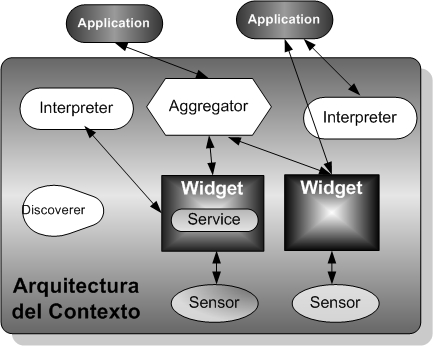
\includegraphics [width=5 in,totalheight=4 in] {Ch1/f2.jpg}
 % .: 0x0 pixel, -2147483648dpi, nanxnan cm, bb=
\caption {Una configuración de las componentes del context Toolkit.}
\label{fig:deytoolkit}
\end{center}
\end{figure}


En el instante en que algún componente contexto se encuentre disponible,
registra sus
capacidades en un discoverer. Esto permite que los \textit{aggregators}
encuentren \textit{widgets} e
\textit{interpreters} y a las aplicaciones encontrar \textit{aggregators},
\textit{widget} e \textit{interpreters}. Un
sensor provee datos para un \textit{context widget}, en cual se encarga de
almacenar el
contexto, puede llamar a un \textit{interpreter} para obtener un mayor nivel de
abstracción de
los datos y luego pone el contexto a disposición (para que pueda ser accedido)
por otros
componentes y aplicaciones. Un \textit{aggregator} recolecta información de
contexto de las
entidades, representadas por los \textit{widgets}. Finalmente, las aplicaciones
pueden consultar
o suscribirse a los \textit{agreegators} (o directamente con los
\textit{widgets}, si se quiere) y llamar a
\textit{interpreters} (si el deseado nivel de abstracción no se encuentra
disponible desde los
\textit{widgets} y \textit{aggregators}).

Estos componentes se ejecutan independientemente de las aplicaciones, asegurando
una
continua adquisición de información de contexto y el uso de múltiples
aplicaciones.
Además, todos los componentes y aplicaciones se comunican entre ellos
automáticamente usando protocolos y lenguajes conocidos. Esto da lugar a que los
programadores que implementaron un particular componente o aplicación puedan
comunicarse con otro componente sin tener conocimiento de los mecanismos usados
para lograr la interacción.


\subsection{Proyecto UWA}

UWA ha nacido de la colaboración entre diferentes grupos de trabajo, por lo que
resulta realmente una agrupación de
propuestas y técnicas. UWA incluye una original propuesta de aplicar la
notación UML para modelar elementos de multimedia que a su vez es heredado
de otra propuesta llamada HDM (Hypermedia Design Model)\cite{HDM11}. Sin
embargo, W2000 ha sido incluida en UWA sólo en la fase de diseño hipermedia,
siendo ambas propuestas diferentes en la fase de definición
de requisitos. Por esta razón han sido incluidos en este proyecto en forma
separada. El proceso de captura de requisitos
en UWA\cite{uwa32} comienza definiendo los diferentes roles de usuario que
pueden interactuar con el sistema, los objetivos
globales del sistemas y la relación entre éstos. El proceso continúa haciendo
un refinamiento de esos objetivos
globales, concretándolos en sub-objetivos. Estos sub-objetivos son estudiados y
refinados para detectar conflictos entre
ellos. De esta forma, se concretizan aún más dividiéndolos en requisitos. Los
requisitos son clasificados en varios tipos:
de \textit{contenido}, de \textit{estructura de contenido}, de \textit{acceso},
de \textit{navegación}, de
\textit{presentación}, de \textit{operaciones de usuario} y de
\textit{operaciones del sistema}. De esta forma, los requisitos se van refinando
hasta que solo pertenezcan a uno de estos grupos. Y finalmente los
requerimientos son asignados a artefactos de diseño o a reglas de customización.
Para definir los objetivos, UWA propone una notación propia, basada en una
plantilla. La definición de los actores y la relación con
los objetivos se hace usando un diagrama basado en casos de uso. Por último,
para definir y refinar los sub-objetivos y los requisitos, utilizan una notación
gráfica propia que denominan grafo de refinamiento de objetivos, el refinamiento
de este grafo permite ir representando la relación entre los requisitos y hacer
un seguimiento para validar la consecución de los objetivos del sistema. Una vez
que los requisitos son detectados, hacen uso de XML para definirlos de una
manera formal.



\begin{quote}
''An ubiquitous web application is a Web application that suffers from the
anytime/anywhere/anymedia syndrome. This means that an ubiquitous
web application should be designed from the start taking into account
not only its hypermedia nature, but also the fact that it must run “as is”
on a variety of platforms, including mobile phones, Personal Digital
Assistants (PDAs), full-fledged desktop computers, and so on. This
implies that an ubiquitous web application must take into account the
different capabilities of devices comprising display size, local storage
size, method of input, network capacity, etc. New opportunities are
offered in terms of location-based, time-based, and personalised
services taking into account the needs and preferences of particular
users. Consequently, an ubiquitous web application must be, on the one
hand, context-aware i.e., aware of the environment it is running in, and
on the other hand it must support personalisation
From: Ubiquitous Web Application Development- A Framework for understanding``

\begin{flushright}
\textit{A. Finkelstein et al 2002}
\end{flushright}
\end{quote} 


Se comienza con la descripción conceptual del framework propuesto en el
proyecto UWA para el desarrollo de aplicaciones web ubicuas basada en el
enfoque de la teoría reflexión (\textit{reflection})



\begin{figure}[t]
\begin{center}
 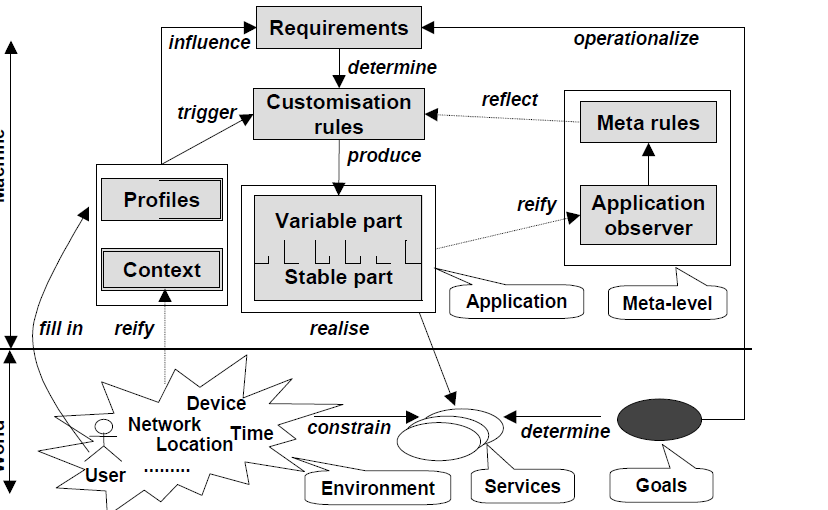
\includegraphics[width=5 in,totalheight=4 in] {Ch1/Figuras/UWAFramework2.png}
 % UWAFramework2.png: 828x510 pixel, 96dpi, 21.90x13.49 cm, bb=0 0 621 382
\caption{Dise\~no conceptual del Framework UWA}\label{fig:uwaFramework}
\end{center}
\end{figure}



\paragraph{Goal}

Goal es un objetivo que el sistema debe alcanzar por medio de la cooperación entre agentes (usuarios y componentes  software) propiamente dicho y dentro
de un entorno. Desde la perspectiva UWA los objetivos son
\textit{inmutables} i.e., no cambia ante cuando se modifica el entorno.
Representa el último objetivo que el servicio está destinado a lograr. Un
cambio en los objetivos significaría cambiar el servicio mismo. A lo largo de
las líneas de \cite{uwa5}, donde un “goal” no es alcanzado por una “acción directa” de uno a más agentes; de otro modo, un “goal” se convierte en un objetivo un tanto
abstracto de largo plazo.

En la Figura \ref{fig:uwaFramework}, los objetivos son de color gris, lo que
significa que ellos son la única parte del marco que no tiene la intención de
cambiar en tiempo de ejecución. Más exactamente, las metas pueden (y deben)
tener una imagen en tiempo de ejecución (ya que su puesta en marcha
en los requisitos de forma dinámica puede cambiar), pero no se pueden modificar
directamente.

\paragraph{Service}

El servicio se puede definir como algo que proporciona valor añadido a uno o más
actores. Un servicio es distinto de
una aplicación, ya que es un concepto mucho más general, que podría ser
proporcionada por ejemplo, por medios distintos de
computadoras. Por ejemplo, si uno de los objetivos es maximizar la usabilidad
del sistema, un servicio puede ser el de proporcionar a los usuario con los
dispositivos de entrada-salida. Este es un ejemplo de diseño centrado en el
usuario, mediante el cual el sistema es sólo un medio para
cumplimiento de las metas de usuario, y no un objetivo en sí mismo. Por lo
tanto, los servicios de pertenecer en el mundo, no en la máquina.


\paragraph{Environment}

Por "Environment" se refiere al entorno en que la máquina
operar. Teniendo en cuenta el medio ambiente es crucial porque influye mucho en
el comportamiento de la máquina.


El entorno cuenta con propiedades para describir una
faceta diferente del medio ambiente. Consideremos el ejemplo de un
servicio de m-commerce. En este caso el medio ambiente abarca cosas tales como
ancho de banda, la ubicación (absoluto y relativo), la disponibilidad del
servicio, las características del dispositivo, y muchos temas más.
Tenga en cuenta que el sistema no tiene control alguno sobre el medio ambiente.
En otras palabras, la máquina debe adaptarse a las
medio ambiente, no al revés. Como cuestión de hecho, si el ancho de banda es
bajo, la conexión es irregular, el
PDA pantalla es pequeña, esto es algo que no puede ser modificado directamente
por el software. El trabajo de un ingeniero de software
por lo tanto puede resumirse como una lucha hacia la meta a pesar del entorno,
todo lo que puede hacer con el
medio ambiente es sentido, y lo describen de la mejor manera posible, pero no
podemos cambiar i


\paragraph{Context}

Contexto se define como la resignificación del medio ambiente en términos de
sus propiedades. En la figura, desde el contexto no salen flechas hacia el
entorno medio ambienta ya que UWA lo interpreta como no modificable. A su vez,
el contexto permite efectuar una descripción del medio ambiente. La mayoría de
las descripciones importantes deben ser dinámicamente actualizables en función 
del cambio posible del medio ambiente. 

El contexto es parte de la máquina, ya que es una representación del medio
ambiente (que a su vez pertenece al mundo real)
dentro del sistema. En otras palabras, el medio ambiente se representa en el
contexto, ya que existe una máquina;
sin esto, el contexto no tendría sentido. Tenga en cuenta que el contexto es la
única parte del sistema que es la aplicación
independiente, en el que se describen las propiedades del medio ambiente
adecuado, independientemente de la aplicación que se va a construir.
Esto está marcado en la Figura \ref{fig:uwaFramework}  por un doble contorno
alrededor de la caja de
contexto. 


\paragraph{Profiles}


A diferencia del contexto, el perfil representa información explicita. Un
ejemplo es el uso de perfil para la personalización de usuarios. El perfil
puede ser dependiente o independiente de la aplicación.


\paragraph{Requirements}

Los Requerimientos representan una de las posibles formas de lograr
una meta. Un requerimiento personaliza un objetivo, ya
que
representa en una forma más concreta los objetivos a corto plazo
que son directamente alcanzables a través de las acciones realizadas por uno o
más agentes. Los requisitos pueden cambiar
durante la ejecución del sistema. El entorno pude sufrir un alto grado de
cambio invalidando los objetivos iniciales. Entonces, cambios en el contexto
puede generar la necesidad de cambios en los requerimientos.

En términos informal, se puede decir que los
requisitos son un ''trade-off'' entre los 
objetivos y la realidad actual. Por ejemplo, el objetivo de una aplicación
m-commerce ubicua podría ser establecida por la alta interactividad de un
usuario. Teniendo en cuenta este
objetivo, si el contexto es favorable (por ejemplo, el ancho de banda, alta,
color de gran tamaño
pantalla, máquina virtual Java disponible) un requisito puede ser "utilizar un
colorido applet de Java para representar el estado de
la cesta de la compra", mientras que si la conexión es lenta o no hay JVM
disponible, el requisito puede ser
mitigado en "utilizar un gif animado de 16 colores."


\paragraph{Application}

La aplicación es la encargada de la implementación de uno o más servicios. La
relación entre aplicación y servicios es de mucho a muchos. Un servicio puede
estar relacionado con varias aplicaciones y una aplicación puede disparar
varios servicios. Un servicio complejo puede estar interactuando con varias
aplicaciones distribuidas. 

Una aplicación está conformada por una \textit{parte estable}, que provee
funcionalidades básicas y una \textit{parte variable}, que se encarga de
efectuar las adaptaciones. Ambas partes están vinculadas por medios de
"ganchos" que implementan la comunicación.



La solicitud se hace por una parte estable, que proporciona la funcionalidad
básica, y una parte variable, que se da cuenta de
la personalización. La parte estable de la aplicación proporciona los ganchos,
los llamados puntos calientes de personalización, que permite la
parte variable para adaptar su comportamiento a las necesidades particulares.
Bajo este aspecto, se asemeja a una orientada a objetos
marco.


\paragraph{Customisation Rules}

Las reglas de personalización (Customisation Rules) 
son el medio por el cual los requisitos se traducen
en la parte variable de la aplicación y
se puede conformar como reglas de producción.


\paragraph{The Meta Level}

El Meta Nivel (Meta level) es una representación de la aplicación en términos
reflectivo. Implementa las eventuales conexiones de la aplicación, esto se
refiere al estado de la aplicación, visto de otra perspectiva, funcionan como
un continuo monitoreo y mantiene una descripción actualizada de su
estado. Esto es necesario ya que el funcionamiento de la aplicación
puede ser influenciada por el medio ambiente, y por lo tanto puede cambiar de
maneras impredecibles. Supongamos, por ejemplo, que un
teléfono móvil está funcionando en un área con fuertes campos magnéticos. En
esta situación, el teléfono puede reportar un buen
conexión, pero la calidad real siempre puede ser baja debido a la interferencia.
En tal caso, el control de la
medio ambiente no es suficiente, y no hay manera de darse cuenta de esta
interferencia que no sea el control de la propia aplicación.
La relación con la aplicación se produce mediante dos vías, donde el
\textit{meta nivel } puede afectar el nivel de
base
funcionalidad por medio de la \textit{meta reglas} que permitirían implementar
la personalización correspondiente. Entonces, ante situaciones particulares
las metas reglas son disparadas y pueden cambiar, a\~nadir o eliminar las
reglas actuales

Un meta nivel de reflexión también se puede emplear para los
requerimientos de control, en el sentido utilizado en \cite{uwa.7}.

en este nivel se implementa una de las principales características que se
pretende poner en obra en esta tesis debido a su relación con
nuestra visión de reconfiguración dinámica. 


Se argumenta que la "manera reflexiva" es una manera limpia y consistente de los
cambios de rendimiento en tiempo de ejecución a la
nivel subyacente (que es finalmente el sistema real como percibida por el
usuario). Este enfoque consiste en la manipulación
las normas de personalización con el fin de conciliar el servicio con los
requisitos. La relación de causalidad, en particular,
el enlace descendente (reflexión), prevé la coherencia entre la descripción del
servicio y el propio servicio.
Técnicas de arquitectura reflexiva puede ser empleado a tal fin [23].




\begin{figure}[t]
\begin{center}
 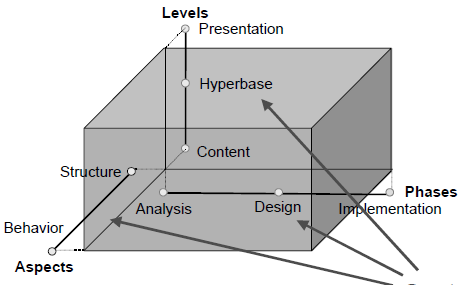
\includegraphics[width=5 in,totalheight=3 in]
{Ch1/Figuras/ScopeCustomisation.png}
 % UWAFramework2.png: 828x510 pixel, 96dpi, 21.90x13.49 cm, bb=0 0 621 382
\caption{Dise\~no conceptual del Framework UWA}\label{uwaFramework}
\end{center}
\end{figure}


\begin{figure}[t]
\begin{center}
 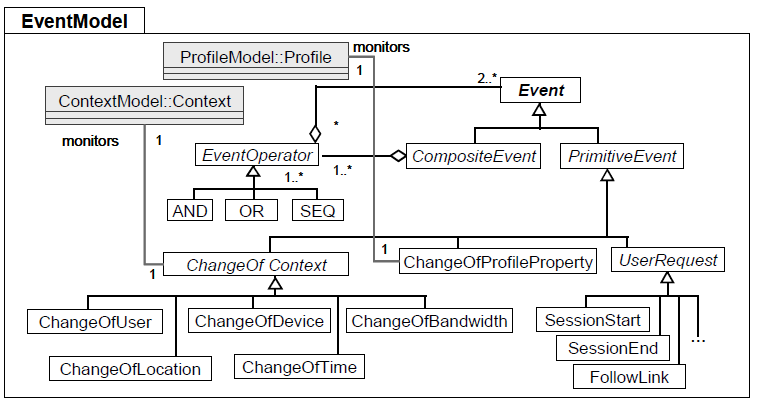
\includegraphics[width=4 in,totalheight=3 in]
{Ch1/Figuras/UWAEventModel.png}
 % UWAFramework2.png: 828x510 pixel, 96dpi, 21.90x13.49 cm, bb=0 0 621 382
\caption{Dise\~no conceptual del Fram}\label{uwaFramework}
\end{center}
\end{figure}



\section{Desde la perspectiva de la Ingeniería de Software}
%...
%(escribir todo esto como teoría de requerimientos).
%...
 
En este capítulo se han explicitado los fundamentos y desarrollos básicos de la evolución
de los SCC. Introducimos la necesidad de que los mismos tuvieran un nivel dinámico sustentado en la teoría de coordinación de
contratos, ya que las definiciones más tradicionales no son suficientes para satisfacer los requerimientos del DHD.

En los capítulos siguientes, se abordará lo inherente a los contratos como pieza de software en base a la arquitectura, el diseño y la
implementación en el campo de la Ingeniería de Software para describir las problemáticas, motivaciones,
el tipo de solución propuesta y un marco de conceptualización-definición
(capítulos: \ref{cap:introduccion} y \ref{cap:dhd} ) en un contexto de alta
complejidad como lo ya expuesto, para tratar requerimientos funcionales derivados del mismo. 

Se tomarán en cuenta todas las convenciones realizadas sobre el
DHD, haciendo foco en adelante sobre lo específicamente tecnológico estableciéndose la interesección interdisciplinar entre las competencias de los usuarios expertos y los ingenieros de software como destinatarios principales de este trabajo de tesis doctoral. 

Es importante para el desarrollo de los próximos capítulos tener presente los
siguientes interrogantes que se constituyen en el sentido sustentador para el
uso de la teoría de Sistemas Colaborativos Sensibles al Contexto en las
aplicaciones que integran al DHD. 



\begin{center}

\begin{tabular}[t]{|l|}
\hline
\rowcolor[gray]{0.7} Preguntas \\
\hline

%\beging{itemize}

\item ¿Cuáles son las variables que definen el contexto del usuario que\\
pueden ser usadas para recuperar información relevante? \\
\hline
\item ¿De qué forma puede modelarse el contexto del usuario? \\
\hline
\item ¿Cómo debe incorporarse el contexto a la búsqueda del usuario?\\
\hline
\item ¿Cómo deben presentarse los resultados derivados del contexto del
usuario?\\
\hline
\item ¿Cuál es la relación costo/beneficio de utilizar el contexto en la
recuperación de información?\\
\hline
\item ¿De qué forma se puede medir la relevancia de los resultados derivados del
contexto?\\
\hline
\item ¿En qué tipo de aplicaciones puede ser útil incorporar mecanismos
que\\
hagan uso del contexto para que logren robustez entregando información
relevante?\\
\hline
%\end{itemize}


\end{tabular}
\end{center}




\section{Conclusiones}

Este capítulo conforma una bisagra entre el universo real del DHD y
las limitaciones de su interpretación computacional. En este sentido, se ha focalizado en determinar cuáles son las fuentes concretas de la
materia prima (el ContextoDHD, sección \ref{sec:contextodhd}) para poder
producir soluciones (el Modelo Evolutivo, sección \ref{sec:sca})
a determinados efectos funcionales del DHD. De la misma manera inicia un
recorrido sobre el estado del arte de propuestas referentes en las que se basa
esta tesis. Entonces, desde este punto se mantendrán nuevas premisas aportadas
que permitirán especializar teorías y conceptos con una nueva entidad
apropiada para el DHD.



% -- Archivo Cap\'{\i}tulo N� 2 --
%%------------------------------------------------- Chapter --------------------------------------------------------
\chapter{arqDHD: Arquitectura de Software para los Dispositivos Hipermediales Dinámicos}\label{cap:arqdhd}

%\pagenumbering{arabic}

\section{Introducción}\label{secc:arqDHD_Introduccion}

En este capítulo se describen los aspectos fundamentales y las decisiones adoptadas basándonos en los modelos y arquitecturas considerados en el diseño e implementación de los Dispositivos Hipermediales Dinámicos (DHD).

Para lograr esto, se lleva a cabo una caracterización de algunos aspectos relevantes en las tareas del proceso de desarrollo de DHD. En este punto, es importante volver a aclarar, que la construcción de un DHD puede partir de una aplicación e-learning, como es el caso de esta tesis basada en Sakai. Este proceso se destaca por la inclusión de artefactos y piesas de software, lo que permite representar, de manera eficiente, la arquitectura necesaria del DHD. Siguiendo este camino, se podrán resolver los requerimientos funcionales del DHD sobre adaptación de servicio según información de contexto mencionados anteriormente (sección \ref{requisitoDHD}).

Todas las decisiones de diseño de la arquitectura sugeridas en este capítulo se denomina Arquitectura del DHD o \textbf{arqDHD}. De este modo se inicia el estudio y definición de los procesos de diseño de los DHD, teniendo en cuenta diferentes tipos de elementos y criterios de interpretación que se ajustan al dominio de aplicación de esta tesis. A continuación se definen los principales elementos de la mencionada arquitectura. 


\begin{itemize}
 
 \item \textbf{Componentes}: Se refiere a los tipos de componentes que podrán adoptar un rol 
 \textit{cliente}, haciendo peticiones a otros componentes con el rol de \textit{servidores}, encargado de brindar esos servicios. \label{lbl:componente} 
 
 
 \item \textbf{Conectores}: Se refiere a los mecanismos de interacción entre los componentes.
 
 \item \textbf{Contratos}: Es el componente de primera clase, provisto con su propio diseño y funcionalidad que deberá ser inyectado a una arquitectura original.
 
 \item \textbf{Subsistemas}: Se utilizará este concepto para representar la idea de que un sistema externos está conectado con algún componente estructural de la arquitectura. 
 
 \item \textbf{Puertos}:  Son los puntos de conexión entre los componentes. Para este trabajo los puertos que intervienen en las estructuras de inyección de los contratos serán componentes de primera clase.
  
 \item \textbf{Artefactos de penetración}: Encargado de establecer componentes de
composición  o conectores internos de la arquitectura con elementos sus
interfaces externas. 

 \item \textbf{Modelo Computacional Subyacente}: Se refiere a la información necesaria donde se explica el funcionamiento en tiempo de ejecución del sistema que implementa la arquitectura. En este trabajo se utiliza para describir algunas cuestiones semánticas referidas a los mecanismos de inyección de los contratos.


\end{itemize}

Conceptualmente \textbf{arqDHD} está definida por aquellos aspectos de la arquitectura que desempeñan un rol protagónico en los DHD. Esta apreciación fue motivada asumiendo que los requerimientos de los DHD se deben resolver a partir de la arquitectura sin tener en cuenta el modo de implementación de aquellos artefactos que la compone.

Además, \textbf{arqDHD} está orientada a la formalización de algunas de las propiedades arquitectónicas singulares en los DHD, promoviendo una mejor representación de la semántica para los conectores y la posibilidad de coordinarlos en tiempo de ejecución.


Existen múltiples definiciones de Arquitectura de Software (desde ahora en más lo llamaremos AS), el Software Engineering Institute‘s (SEI)\cite{arquitectura23} recoge 75 definiciones distintas del término Arquitectura del Software. Para este capítulo es imprescindible identificar los criterios que se tendrán en cuenta, para un mejor entendimiento de las decisiones adoptadas. En este sentido, se seleccionaron dos definiciones que se ajuste más a la acepción que toma esta propuesta y especializarla en el dominio de las aplicaciones Web colaborativas.

\begin{quote}

La arquitectura es la organización fundamental de un sistema
expresado mediante sus componentes, las relaciones entre cada uno de ellos y
con su entorno, y los principios que guían su diseño y su evolución.

\begin{flushright} \textbf{IEEE Architecture Working Group} \end{flushright}

\end{quote}

Se trata de una definición consensuada por un organismo internacional, por ese motivo es un intento de simplificación y unificación de las definiciones existentes por los diferentes expertos en la materia. Lo primero que destaca de esta definición, es que establece al componente \hyperref[componente]{lbl:componente} como la unidad arquitectónica para el tipo requerimientos arquitectónico del DHD. El componente es un concepto demasiado ambiguo y que en ocasiones puede hacer referencia desde un subsistema hasta un componente cliente. Además, es importante resaltar el hecho de que la definición señala a la AS como responsable de establecer los mecanismos para guiar el diseño y su evolución, ya sea mediante la captura de los requisitos no funcionales o mediante el uso de patrones. De esta manera, Booch \cite{Booch15} señala la importancia que tiene la AS en la evolución de un sistema, indicando que
la presencia de una arquitectura estable en un sistema, asegura las bases sobre las cuales un sistema puede 
volucionar continuamente con los mínimos desajustes y trabajo.

Sin embargo, buscando una definición que fuera menos ambigua y aportara un poco más contenido a la hora de modelar el tipo de arquitectura que se ajuste al DHD seguimos con otra que incorpora el concepto de propiedades:

\begin{quote}

La arquitectura es la descripción de los subsistemas y componentes de
un sistema de software y las relaciones entre ellos, típicamente representado mediante vistas que muestran las propiedades funcionales y no funcionales más relevantes  

\begin{flushright} \textbf{Buschmann} \cite{arqModulos} \end{flushright}

\end{quote}


En esta definición de AS, aparecen los subsistemas junto con los componentes como unidades arquitectónicas. \textbf{arqDHD} se basa en esta aproximación capturando tanto los subsistemas denominados contratos sensibles al contexto, como los componentes en los modelos de integración (sección \ref{sec:integracion}) y de configuración (ver capítulo \ref{cap:contratos}), a la hora de representar la arquitectura Web.

Otro aspecto a destacar de la definición, es indicar que la AS debe representar los aspectos más relevantes del sistema, abstrayéndose de cierta información menos importante para esta tesis.

Hay que recordar que la arquitectura no es solamente una referencia estructural, (en ocasiones es entendida erróneamente como la estructura de la aplicación), sino que provee un mecanismo natural de integrar varias vistas del sistema. Aquí  es donde se torna relevante el concepto de vista y perspectiva de un sistema que.   Estas vistas pueden ser tanto estructurales, funcionales y de comportamiento. Como se muestra a partir de la sección \ref{secc:arqDHD}, en \textbf{arqDHD} se utilizan vistas funcionales definidas por otras aproximaciones que son representadas de forma concurrente a la arquitectura propuesta. 

En el capítulo anterior se han repasado las principales características y elementos que componen los \textbf{arqDHD} para brindar las propiedades de \textbf{coordinación de contratos sensibles al contexto}, que formarán parte de las componentes esenciales de la arquitectura propuesta.

Desde esta perspectiva se podrá observar las posibilidades adaptativas propias del dominios de aplicación y los logros obtenidos en estos campos. Una vez determinado para qué sirven, el siguiente paso es describir cómo funcionan. 

La arquitectura del sistema está formada por cuatro subsistemas, cada uno de
ellos tiene una misión específica y determinada. Su diseño busca separar conceptos funcionales,
mejorando de esta manera la evolución independiente de cada subsistema
\ref{arquitectura1}. Para esta representación se tuvieron en cuenta algunas de
las características de los principales patrones para la representación de
arquitectura, a través de los patrones de distribución definidos por diversos
autores Buchmann et al. \cite{Buchmann}, Conallen \cite{Conallen}, Trowbridge\cite{Trowbridge}


\section {Conceptos Fundamentales}


Ahora se revisarán los conceptos arquitectónicos más relevantes que fueron
necesarios tratar en las etapas de diseño teniendo en cuenta dos tipos de factores importantes para la naturaleza de la problemática e hipótesis abordadas en este capítulo. En primer orden, se expondrán los estilos de arquitectura estudiados de los avances que se sintetizan en esta tesis, en función de los framework e-learning consolidados y de posibles futuras propuestas. En segundo orden, se tendrá en cuenta todo lo referido con metodologías de diseño y construcción de las arquitecturas. Todos los esfuerzos que se puedan condensar sobre estos dos factores (estilos y metodología) repercutirán en la factibilidad de la concreción de la hipótesis de inyección de contratos.   

Anteriormente, se mencionó que una arquitectura de software
viene determinada por los componentes –elementos básicos caracterizados por una
interfaz segmentada en \textit{puertos} y \textit{conectores} que la constituye
constituyen, así como por una serie de conexiones o enlaces específicos, que
definen la unión de todos ellos formando una estructura. A esta estructura se
le da el nombre de configuración y suele considerarse insertada en una
jerarquía, independientemente de su granularidad. Ocasionalmente, la
configuración no se describe de manera monolítica, sino que se estructura en
diferentes vistas, cada una de las cuales se concentra en un aspecto diferente.

Para la creación de una arqDHD no solo hay que obtener una configuración concreta, además, hay que establecer una serie de patrones que puedan representar cualquier tipo de inyección de contratos de un framework Web colaborativo. En este sentido, se puede hablar de la definición también de un estilo \cite{arqEstilos}. En definitiva, es la definición de todos
estos aspectos la que determina una visión concreta de la arqDHD; a este fin se dedicarán los apartados siguientes.



\subsection {ComponenteDHD} 


El siguiente paso hacia la creación de una arqDHD es estudiar las principales componentes del DHD. Esto se refiere, en términos globales, a cada una de las partes o unidades de composición –por definición– en las que se subdivide la funcionalidad de un sistema o subsistema DHD y cuya unión da lugar al sistema completo DHD. En su sentido más genérico, puede hacer referencia a cualquier tipo de elemento estructural, esto es, integrado en una estructura; es precisamente con este significado con el que lo llamaremos \textbf{compontesDHD} de la arqDHD en esta tesis.

El término de componenteDHD se limita a la arquitectura arqDHD, no se utilizará  de la habitual manera de componentes en múltiples campos de la Ingeniería de Software desde la propuesta realizada por Douglas McIlroy \cite{Douglas} en la célebre conferencia de la Otan en Garmisch-Patenkirchen. En realidad, su connotación más habitual hace referencia más bien a aspectos de implementación, vinculados a los estudios de Desarrollo Basado en Componentes. 

En este trabajo se parte de una definición genérica de componentes para luego establecer una adecuada para \textbf{componenteDHD}


\begin{quote}

\textit{Un componente es una unidad de composición de aplicaciones
software, que posee un conjunto de interfaces y un conjunto de requisitos y que puede ser desarrollado, adquirido, incorporado al sistema y compuesto con otros componentes de forma independiente, en tiempo y espacio.
}
\begin{flushright} Clemens Szyperski \cite{cacic2007.7} \end{flushright}

\end{quote}


En el contexto del desarrollo de componentes de los DHD, se deben
hacer adaptaciones, extensiones y agregados para romper de alguna manera con el 
alto grado de encapsulamient, ya sea por razones de abstracción, de seguridad o por
motivos comerciales, con el propósito de agregarles posibilidades de
adaptación mediante el uso de envolventes, adaptadores o mediadores
(ver sección \ref{adaptadoresymediadores}). Ese papel ha sido asumido
en Arquitectura de Software, normalmente, mediante el uso de
conectores desarrollados específicamente para la ocasión. Por ello, no
es extraño que cada vez más autores propongan un cambio
en este sentido, especialmente en aquellos sistemas colaborativos como el DHD, de manera tal que todo componente conste de una interfaz privilegiada que permita algún
tipo de acceso, con grados relativos de seguridad, a detalles internos. Esto
define lo que se ha dado en llamar una caja gris \cite{cacic2007.7}, un concepto ya
propuesto con anterioridad para la Orientación al Objeto \cite{KLM+97, HL95} y que
será una de las principales ideas que se adoptó en esta tesis para resolver los
RequerimientoDHD (sección \ref{secc:requerimientosDHD}). De este modo, se obtendrá
la definición de componentes como una caja gris, como un simple efecto
secundario del relacionamiento con contratos sensibles al contexto.

\begin{def}
Un \cite{componenteDHD} es un tipo de componente, de la arquitectura y estilo arquitectónico planificado, agregado para convertir un framework colaborativo Web en un  Dispositivo Hipermedial Dinámico (DHD). Además, interviene directamente en cualquier proceso de aprendizaje \textbf{prodA} \ref{prodA}.
\end{def}


\subsection{ConectorDHD}

Los conectorDHD se ajustan al concepto estándar de conectores que procede principalmente de los trabajos de Mary
Shaw  \cite{SG96}, a partir de su experiencia en Unicon \cite{SDK95}. En un célebre artículo \cite{Sha94}, propuso considerar por separado las abstracciones relativas a la funcionalidad (el componente) y a su interacción (el conector). De este modo, se realiza una clara separación de intereses, que permite ampliar el nivel de abstracción y aumentar la modularidad del sistema.

Sin embargo, lo que se propone no es simplemente disponer de dos tipos de
componentes, sino de distinguir dos elementos diferenciados, con funciones muy
dispares. Los componentes normales –elementos de computación– realizan una
tarea sin preocuparse de cómo se relacionan con el resto del sistema; por su
parte, los elementos e interacción, denominados conectores, son los que se
encargan de resolver todas las cuestiones relativas a la comunicación de los
primeros.

Shaw insiste en que los conectores deben ser considerados como elementos de
primera clase, que tienen significado por sí mismos. Esto quiere decir que no
serán definidos en función de otros elementos, ni diseñados específicamente
para un componente, sino que podrán ser extraídos y considerados en otro
contexto.

La forma más elemental de ver a un conector es como la encarnación de un
protocolo de comunicación, entendido en su sentido más amplio. En general,
cualquier artificio –o artefacto– que permita comunicarse a dos o más elementos
es un conector. Por ejemplo, la llamada de procedimiento es un tipo clásico de
conector.

No obstante, la definición del concepto supone que hay dos tipos de vínculo
entre los distintos elementos de una descripción arquitectónica: por una
parte, el propio conector expresa la interacción existente entre varios
componentes pero, por otra, esto exige establecer, a su vez,
el tipo de enlace que relaciona a cada componente con un conector determinado. Esto significa que este enlace recibe normalmente el nombre de adjunción o attachment. Sin
embargo, a lo largo de esta tesis lo denominaremos simplemente como “conexión”,
término que consideramos más intuitivo, menos forzado y más cercano a su uso
convencional en español \footnote{En inglés, del mismo modo, preferimos el
término más general de binding, utilizado en algunos lenguajes sin conectores,
como \δarwin, aunque es tal vez más cercano a aspectos formales o
de implementación.}


Es importante señalar que existen ciertas diferencias de matiz en cuanto al
uso de la palabra conector. Podría decirse, incluso, que se utiliza con
dos sentidos diferentes aunque relacionados.
Por un lado,  suele entenderse que la propuesta original de Shaw exige la
definición de un nuevo tipo de elemento, análogo a un componente y que se
describe del modo indicado. Por otro lado, también se puede mencionar la palabra
conector, de modo general, haciendo referencia a cualquier interacción
explícita entre dos componentes, lo que incluye a los \textit{bindings}
de δarwin (sección \ref{darwin}) o a las conexiones de Rapide (sección
\ref{Rapide}). Este es, por ejemplo, el sentido en que lo usa Medvidovic, cuando 
señala que la definición de conectores es uno de los rasgos que
caracterizan al modelo conceptual de \textbf{arqDHD} (figura \ref{fig:arqAreas}). Sin embargo, en pro de la claridad, en esta tesis se utilizará la palabra únicamente en el 
primer sentido, es decir, como elemento de primera clase, haciendo siempre una distinción
explícita entre conector y conexión.


Incluso en su forma más básica, esto es, cuando se los considera como simples
conexiones, la enumeración de enlaces o asociaciones explícitas entre los
elementos de un sistema proporciona una descripción, siquiera parcial, de su
estructura, es decir, de su arquitectura. En \cite{arqDHD} los conectores importantes permiten, directa o indirectamente, funcionalidades de adaptabilidad en los procesos prodA.

\begin{comment}
ya está reforzando su capacidad para especificar configuraciones, lo
que constituye la tarea principal de cualquier Adl. De hecho, uno de los
primeros trabajos sobre Rapide [LVM95], uno de los lenguajes con un modelo de
conexión más simple, demuestra que esta característica, por sí
sola, resulta suficiente para distinguir con claridad un Adl de un
lenguaje orientado al objeto convencional. Tal vez, sugerir la posibilidad de
una confusión entre estos dos tipos de lenguajes resulte ahora extraño; aunque,  debido al énfasis que ambos hacen en el concepto de encapsulación,
éste es un punto que fue ampliamente debatido en su momento [Cle96], e incluso
reaparece, todavía hoy, de manera ocasional.

\end{comment}

Se puede ver a los conectores de dos maneras, a
menudo antagónicas, pero que no tienen por qué serlo: como una
especificación o como una simple implementación. El mejor ejemplo que puede citarse referido a una especificación son los conectores de Wright, en tanto que los conectores 
de Unicon son un ejemplo adecuado de una simple implementación. En un lugar intermedio podrían
situarse los de C2. Para Wright los conectores son, ante
todo, especificaciones que indican qué es lo que se espera de un componente en
una interacción dada. En otras palabras,  se trata ante todo de indicar el papel de cada
uno de los componentes en cada uno de los protocolos ya que si la especificación del
conector se corresponde con las de los componentes, entonces se puede verificar la
corrección del sistema.

Para Unicon, en cambio, un conector no es más que una implementación de un
Protocolo cuyo objetivo es, ante todo, evitar que el diseñador del componente
tenga que preocuparse de los aspectos de interacción. Por esta razón, se plantea
como un elemento reutilizable que puede ser conectado a un componente en un
momento dado y que se encarga desde ese momento de realizar las interacciones
apropiadas. Nikunj Mehta \cite{MMP00} ha hecho un estudio exhaustivo de todo aquello
que ha sido o es considerado un conector; si bien puede ser identificada como el principio de una
taxonomía que se hace claramente necesaria, no constituye más que un trabajo
preliminar y, lamentablemente, no parece haber tenido continuidad. No obstante,
un trabajo como el de él, completamente desarrollado, será imprescindible para
que el concepto pueda llegar a alcanzar todo su potencial.

Para este capítulo se decidió caracterizar a los conectores a nivel de diseño, a fin de obtener una documentación conceptual adecuada que permita entender las decisiones que se toman en función de requerimientos funcionales que refieren a la adaptabilidad y a los esquemas originales de los framework e-learning. 

Una comprensión adecuada de la naturaleza del
conector caracterizados en \textbf{arqDHD} permite la definición de un álgebra de conectores que, combinándolos, posibilite la descripción de interacciones aún más elaboradas, en las que se ha elevado el nivel de abstracción. 

Debe tenerse en cuenta que el propio concepto de conector se puede poner en discusión en una arquitectura planteada del estilo de arqDHD. Aunque se trata de una idea generalizada y es aceptada de manera común, no todos los autores están plenamente convencidos de su necesidad. Algunos, entre los que se destaca Jeff Kramer, opinan que la existencia de los conectores distorsiona la naturaleza compositiva de una arquitectura de software que queda afectada de manera negativa. Ciertamente, mientras que la composición de dos elementos de estructura similar –dos componentes– resulta fácil de expresar, ya sea de manera formal o informal, es claro que la introducción del conector como un segundo tipo de elemento complica la situación. No se trata simplemente de una
yuxtaposición de funcionalidades, sino que ha de considerarse el tipo de
composición que define el conector. Existen, además, una serie de problemas
derivados, como es la diferencia precisa entre componente y conector acerca de cuál es
la naturaleza exacta de un compuesto intermedio en la cual alguno de los
extremos –o roles– de un conector quedase libre. Justamente, en arqDHD tenemos el componente contratosDHD que se analizará desde una perspectiva en la que se desempeña con el rol de conector.

Algunas argumentaciones enuncian que un “componente de interacción”, concebido de manera equivalente a un conector pero definido de forma análoga a otros componentes, mantiene las posibilidades de reutilización sin perder la composición. Aunque esto rechaza la posibilidad mediante la cual era considerado como una abstracción básica, no contradice
explícitamente la propuesta de Shaw que plantea que el mero hecho de plantear la diferencia
entre las dimensiones de composición e interacción es ya importante, constituyendo su verdadera esencia.

En definitiva, la noción de conector se ha convertido en uno de los rasgos
definitorios del campo: ya sea como un componente específico, como una conexión
compleja o como una noción por propio derecho, siempre aparecerá, de algún modo,
en toda descripción arquitectónica. En esta tesis, definiremos conectorDHD a un tipo de conector que está
fuertemente ligado a la noción de contrato (siguiendo los lineamientos de Meyer
\cite{Meyer}), especializándolo para un determinado tipo de conexión,
manteniendo cierto nivel de expresión y cumpliendo propiedades específicas de
los DHD.


\begin{defi}
Un \textbf{contectorDHD} está formado por las conexiones entre componentes de la arquitectura arqDHD que permiten construir un artefacto de software donde el flujo de datos depende de un contratoDHD.
\end{defi}


\subsection{PuertoDHD} 

El concepto de puerto es cercano al de conector, pero no debe ser confundido con
éste bajo ningún concepto. Se denomina con este nombre a cada uno de los
puntos por los que un componente puede realizar cualquier tipo de interacción;
dicho de otro modo, es cada uno de los fragmentos en los que se segmenta el
interfaz de un componente.

En definitiva, hace referencia a un punto de entrada o de salida de la caja
negra que es, de hecho, el componente. Diversos autores lo ven y lo denominan de
distinto modo y la analogía que implícitamente se establece no es idéntica
en todos los casos. 

Los puertos se han denominado de diferente manera en distintos lenguajes; así,
en \emph{Wright} se llaman puertos en los componentes, pero roles en los
conectores,
mientras que en \emph{Unicon} reciben el nombre de jugadores. En \emph{δarwin} se
conocían inicialmente como puertos, para después pasar a llamarse nombres de
interfaz, de manera consistente con su semántica en cálculo-π.

Actualmente se conocen como portales, un nombre que expresa total neutralidad
respecto del signo de la interacción ya que los mismos pueden ser portales de entrada o de
salida.

Habitualmente los puertos se agrupan definiendo una interfaz. En algunos
lenguajes se permite, incluso, que definan más de una y, en algunos
sistemas se asume que el puerto está sub-estructurado en varios puntos de
entrada y, por tanto, se define en tu totalidad como una interfaz completa. En este sentido, puede tomarse como ejemplo el caso de Koala \cite{vOvdLKM00}.

En arqDHD, en las partes de diseños donde se instrumenta la inyección de los contratosDHD está fuertemente orientado a los conectores cumpliendo el rol de interfaces ajustadas a cada una de los componentes y artefactos que compone la infraestructura de inyección. 


\begin{defi}
Denominaremos como \textbf{puertosDHD} a las interfaces de los componentes de arqDHD que intervienen en cualquier tipo de conexión entre los componentes DHD denominadas contratosDHD, condicionalesDHD, reglas de contratos y sub-sistema sensible al contexto de una arquitectura del tipo arqDHD.
\end{defi}



\section{Visión arquitectónica de los DHD}

La presente sección tiene como objetivo iniciar el proceso de definción de los lineamientos que permitan describir algunas de las
características que se estudiarán sobre arqDHD. Se comienza con el
recorrido de diferentes propuestas que involucran determinados aspectos de
ArqDHD y sus interconexiones conforman su espacio de estudio.

\subsection {Propuestas de Arquitectura del Software para los DHD}

A diferencia de lo que ocurre en la parte funcional de la aplicación Web, es
difícil establecer criterios y formalismos en cuanto a qué aspectos
(incluyendo los conceptuales) es necesario capturar en la arquitectura Web
colaborativa. Por lo tanto, es importante mostrar los diferentes tipos de
aproximaciones existentes, cuáles son sus principales características comunes y
qué aspectos comparten con \textbf{arqDHD}. De esta manera, comienzan a identificarse las características que distinguen a arqDHD del resto de aproximaciones que representan la arquitectura de las aplicaciones Web.

\begin{itemize}

\item  \textbf{REST}

El Representational State Transfer (de aquí en adelante, REST) \cite{31} consiste en un
estilo arquitectónico para aplicaciones Web distribuidas. El REST está basado en la definición de un conjunto de restricciones arquitectónicas centradas en el dominio de las aplicaciones Web.

Así, el REST propone un proceso de definición de su estilo arquitectónico apoyándose en la introducción de restricciones sobre otros estilos arquitectónicos reconocidos dentro de la arquitectura del software como Client/Server, Layered, Cache, etc.

En este sentido, el REST hace uso de tres vistas arquitectónicas (Proceso, Conector y Datos) para especificar la arquitectura Web. En su especificación ignora los detalles de la implementación del componente y la sintaxis del protocolo para enfocarse en los roles de los componentes, las restricciones de las interacciones con otros componentes y su interpretación de los elementos de datos significativos. Las restricciones de REST se fundamentan en los componentes, conectores y los datos que definen la base de la arquitectura Web.

El objetivo de REST es poder actuar como una guía para que los diseñadores de aplicaciones Web definan el conjunto de requisitos no funcionales relevantes para la aplicación.

Ejemplos de este tipo de requisitos son la obtención de una buena escalabilidad, despliegue independiente, reducción de la latencia de interacción entre los componentes, refuerzo de la seguridad o la encapsulación de los sistemas legados.

La sintaxis utilizada para modelar la arquitectura no se basa en el uso de
estándares de modelado, ni tampoco propone su formalización mediante metamodelos. Esto hace difícil su especificación mediante herramientas comerciales.

La clasificación de tipos de componentes realizada por el estilo arquitectónico
REST ha servido de referencia para la definición de la tipología de componentes
definida por los estilos de \textbr{arqDHD}.


\item \textbf{Architecture Recovery of Web Applications}

Hassan y Holt \cite{42} consideran que las aplicaciones Web se convertirán en los
próximos años en sistemas legados de difícil mantenimiento. Partiendo de esta
base, proponen una aproximación que realice una recuperación de la arquitectura
de las aplicaciones Web a partir de su implementación. El objetivo de esta
ingeniería inversa de la arquitectura es mejorar el mantenimiento de la
aplicación, al hacerla más entendible para los desarrolladores.

La aproximación define un conjunto especializado de parsers/extractores que
analizan el código fuente y binario de las aplicaciones Web existentes y
obtienen un conjunto de diagramas de arquitectura situados a diferentes niveles
de abstracción.

La aproximación establece la definición de un conjunto de cinco componentes
identificados como comunes dentro de la arquitectura Web: Static Pages (Páginas
Estáticas), Active Pages (Páginas activas de servidor), Web Objects (Componentes
de servidor), Multimedia Objects (objetos multimedia como imágenes, video y
sonido) y Databases (bases de datos).

La representación de la arquitectura se basa en un conjunto de tres modelos que
de forma progresiva reducen los detalles obtenidos en la recuperación de datos,
para mostrar únicamente la información relevante para la arquitectura. El primer
modelo es conocido como ELS: Entity-Level Schema. Este modelo es el nivel de abstracción más
bajo y muestra las relaciones entre los elementos que viven dentro de los
componentes Web, tales como objetos, tablas, variables, etc.. A partir de este modelo se
definen las transformaciones necesarias para subir el nivel de abstracción hasta
el modelo Component-Level Schema (CLS) . El modelo CLS representa las relaciones entre los
componentes de la aplicación Web (StaticPages, ActivePages, Databases, etc.). El
último nivel de abstracción es el modelo ALS (Abstract-Level Schema) que
representa las relaciones entre los elementos de mayor granularidad, los
subsistemas y los componentes que contienen.

Los diferentes modelos representados en esta aproximación se basan en esquemas
(Schemas) que son básicamente modelos Entidad-Relación (EER). 

\item  \textbf{WAE: Web Application Extension of UML}

La propuesta WAE \cite{24} (Extensión para las aplicaciones Web) definida por Jim
Conallen propone un conjunto de modelos UML cercanos a la implementación que,
dentro del contexto del Proceso Unificado de Rational (Racional Unified Process
\cite{47}), giran en torno a la arquitectura de la aplicación.
Conallen basa la descripción de la arquitectura de las aplicaciones Web en el
conocido trabajo de Kruchten —The 4+1 View Model of Architecture“ \cite{64},
estableciendo los artefactos utilizados en cada una de las vistas que define
Kruchten para el desarrollo de las aplicaciones Web.

Conallen, partiendo de la idea que una arquitectura nunca aparece de la nada, se
basa en un conjunto de patrones de arquitectura para su definición en la fase de
diseño. Por un lado, adapta patrones comunes que considera particularmente
adecuados para las aplicaciones Web, como son: Façade de Gamma et al. [36], Page
Composition y Template Page. Otros patrones específicos para la capa
de presentación son Thin Web, Thick Web y Web Delivery.

Sin embargo, donde verdaderamente la arquitectura comienza a tomar relevancia
es dentro del proceso definido por Conallen en la fase de diseño. En esta fase
define WAE que incluye un conjunto de tipos de componentes especializados en el
dominio de las aplicaciones Web (p.e. Server Page, Client Page, HTML Form,
etc.). La definición de cada uno de los componentes la realiza mediante el
mecanismo de perfiles proporcionado por UML. Así, una vez definido el WAE es posible representar una
aplicación Web muy detalladamente, acercándose al nivel de implementación
concreta, con la introducción de aspectos dependientes de ASP y JSP.
A partir de la representación en WAE, existe un mecanismo de generación
automática que permite obtener el esqueleto de los diferentes componentes.

\item \textbf{WebArquitect}

WebArchitect \cite{112} es otra propuesta que se centra en la arquitectura y en las
funciones de los lugares Web, más que en la apariencia de cada página. Este
método comienza con una actividad de análisis en la que, mediante el modelo
Entidad-Relación, se puede representar el dominio del problema. A continuación, un
análisis de escenarios determina cómo los usuarios potenciales interactúan con
la aplicación Web para cumplir los objetivos de negocio. A partir de las fases
de análisis, la arquitectura de la aplicación es diseñada en la fase de diseño
arquitectónico. La arquitectura es representada mediante un modelo denominado Relationship Management Data Model for Web-Based Information Systems (de aquí en adelante será citado por sus siglas: RMDMW) que
consiste en una extensión del modelo propuesto por RMM \cite{48}, ya que se introducen eventos, roles y productos.

Mediante el modelo RMDMW el diseñador determina la navegación y el modo de mapear la
navegación a las diferentes páginas.

El método también define atributos para cada página, que son utilizados para el
mantenimiento de la misma. De esta manera, la  implementación y el mantenimiento de la aplicación
resultante es soportada por una herramienta del mismo nombre, que permite a los
diseñadores manipular de forma directa meta-enlaces entre páginas organizadas en
un árbol jerárquico. Por otro lado, la visualización de las aplicaciones
resultantes se realiza mediante un cliente Web denominado Pilot-Boat, que navega
y deja que los usuarios colaboren a través de los lugares Web.

\item \textbf{WAM (WebComposition Architecture Model)}

WAM \cite{WAM} es una aproximación muy reciente basada en la extensión de la
reconocida aproximación WebComposition \cite{WebComposition}. WAM introduce una descripción
arquitectónica que sirve como mapa para el mantenimiento de las trazas de las
interrelaciones entre diferentes aplicaciones Web federadas. Las aplicaciones
Web federadas se basan en la idea de las aplicaciones Web que comparten
componentes y elementos realizados por múltiples proveedores a lo largo de la
Web. Entre los artefactos modelados están los servicios Web, las propias
aplicaciones Web y las zonas organizacionales de control que están sujetas a la
evolución en el sentido de la aproximación WebComposition.

WAM persigue hacer comprensible mediante los modelos la estructura técnica de
la federación a los actores (stakeholders) que intervienen en el desarrollo de
la aplicación Web (p.e. arquitectos, desarrolladores y administradores).

WAM se basa en DSLs, lo que se conoce con el nombre de: Domain-Specific Languages; a fin de representar los diferentes
elementos identificados como relevantes en la arquitectura Web los cuales son:
“service”, “application”, “data provider”, “process unit”, “invocation” y “trust relationship”. A partir de los elementos del modelo, se establece un mapeo
a un lenguaje llamado WAM-XML que sirve de base para su tratamiento en
herramientas y para dar soporte a los sistemas. 



\item \textbf{OOHDM-Java 2}

OOHDM-Java 2 \cite{OOHDM} es un trabajo que propone una línea de producto en J2EE para
simplificar el desarrollo de aplicaciones utilizando la conocida aproximación de
Ingeniería Web OOHDM. OOHDM-Java2 es una arquitectura que permite
desacoplar las decisiones de diseño relacionadas con el modelo de dominio de
aquellas relacionadas con la navegación y la arquitectura de interfaz.
OOHDM-Java 2 tiene asociado un framework J2EE que extiende el concepto del
patrón de Buchmann et al. \cite{Buchmann} Model-View-Controller y realiza una separación de
los nodos de navegación de sus interfaces. Así, introduce la idea de objeto de
navegación, reconociendo el hecho de que la navegación puede ser dependiente del
contexto. La estructura de OOHDM-Java 2 contiene elementos que configuran una
arquitectura que persigue las mejores prácticas y los mejores resultados de
mantenimiento. Este esqueleto (framework) es instanciado para las diferentes
aplicaciones definidas en OOHDM, mediante un conjunto de tareas definidas que
debe seguir el diseñador para su utilización.

\end{itemize}



\subsection {Propuestas basadas en el Desarrollo Dirigido por Modelos para
Aplicaciones Web}

Ahora bien, el último conjunto de propuestas de interés para este trabajo es aquel que se
basa en el paradigma de ingeniería dirigida por modelos (MDE) \cite{MDE} para el
desarrollo de las aplicaciones Web. El modelo MDE proporciona como principales ventajas el
dotar de un mecanismo de trazabilidad desde los modelos hasta la implementación
mediante el uso de las transformaciones. Sin embargo, debido a la juventud de
MDE son pocas las herramientas disponibles hasta el momento y la mayoría de las
implementaciones realizadas por las aproximaciones no se basan en
transformaciones formales, sino que las implementan directamente mediante
generación de código. Otro de los aspectos a considerar es el uso de los modelos
definidos en la Ingeniería Web para representar las diferentes vistas: mientras
que algunas aproximaciones definen sus propios modelos, otras se valen de
trabajos reconocidos para definir sus modelos


\begin{itemize}

\item \textbf{Model-Driven Development of Large-Scale Web Applications}


Tai et al. \cite{Tail} definen una aproximación basada en MDA para el desarrollo de
aplicaciones Web de gran tamaño. Para ello, proveen un conjunto de modelos
basados en un meta-modelo que es usado como contrato principal entre los
desarrolladores.

El meta-modelo juega un papel fundamental al realizar una división en
sub-aplicaciones que proveen la especificación que todos los artefactos deben
cumplir. El me-tamodelo se ha definido conforme a la arquitectura propuesta para
la plataforma J2EE. En un futuro se pretende hacer que el meta-modelo sea general
para otras plataformas.

Los modelos definidos por la aproximación son: (1) el modelo de transición de
páginas (navegación entre los nodos mediante un gráfico), (2) modelo de flujo de
página (composición de la interfaz de una página) y el (3) modelo de datos
(información que se almacena a partir de las páginas). Para la definición de
estos modelos, Tai no se ha basado en los modelos definidos dentro de la
Ingeniería del Software.

Acompañando a esta aproximación se ha definido una herramienta llamada WAST que significa: Web Application development Support Tool. La WAST provee un conjunto variado de
generadores de código (básicamente esqueletos) y mecanismos de validación de
código para comprobar que los artefactos definidos en las diferentes vistas
(p.e. los JSPs (Java Server Pages)) son compatibles con el modelo.
Como parte del proceso de desarrollo se deben definir los diferentes actores
(stakeholders), cada uno de los cuáles debe seguir las reglas impuestas por el
meta-modelo. Estos actores son el diseñador de pantallas, el mantenedor de
modelos, el programador de lógica de negocio, el programador de objetos de
servidor y el ensamblador de la aplicación. Los programadores deben rellenar
aquellos huecos que los generadores de código dejan, siempre verificando que el
código introducido respeta el modelo.

\item \textbf{MIDAS} 

La MIDAS \cite{MIDAS} es la metodología dirigida por modelos para el desarrollo de aplicaciones
Web. Esta metodología aplica un meta-modelo MDA a la plataforma Web utilizando
XML y la tecnología objeto-relacional. MIDAS propone diferentes modelos PIM y PSM
y define algunas reglas de mapeo entre los modelos.

Los modelos independientes de la plataforma (PIM) propuestos por MIDAS están
definidos utilizando el estándar UML \cite{UML}. Los modelos PIM están constituidos
por contenido, navegación y presentación. Para representar los distintos modelos
MIDAS se basa principalmente en UWE \cite{UWE}.

MIDAS también define un conjunto de modelos dependientes de plataforma (PSM)
que representan cada una de las vistas definidas como PIM. Así, para representar
el modelo de contenido dependiente de plataforma, se ha valido de la tecnología
objeto- relacional. Sin embargo, para representar la navegación y la
presentación ha utilizado XML. 

MIDAS propones únicamente las guías para realizar las transformaciones PIM-
PIM, PIM-PSM y PSM-PSM necesarias para completar su desarrollo. Actualmente,
está trabajando en implementar las transformaciones para obtener la aplicación
final sobre plataformas como J2EE y dot NET.


\item \textbf{Model-Driven Development Process for UWE}

El reciente trabajo \cite{58} redefine el proceso de UWE estableciéndose como un
proceso de desarrollo dirigido por modelos (ahora llamaremos MDD-UWE). Para su
definición se ha basado en los principios de MDA, usando los estándares OMG para
la definición de sus modelos y transformaciones. El proceso de desarrollo de
MDD- UWE consiste en un conjunto de modelos y transformaciones cuya
especificación está soportada por meta-modelos y reglas de transformación. Los
meta-modelos son el meta-modelo de MDD-UWE [59], el meta-modelo Web Requirements
Engineering metamodel (WebRE) \cite{WebRE} y, además, utiliza el meta-modelo de nuestra
propia propuesta arqDHD (Meliá \& Gómez \cite{Melia}).

\begin{comment}

El proceso de desarrollo especifica los requisitos funcionales basándose en el
trabajo de cite{} para su automatización de requisitos a contenido funcional. Los
aspectos funcionales son especificados simultáneamente con los modelos de
arquitectura especificados por arqDHD que posteriormente son integrados. Existe
otra alternativa para la integración de la arquitectura con un modelo —“Big
Picture”, es decir, un modelo que integra ya las tres vistas funcionales
(presentación, contenido y navegación).

\end{comment}

Las transformaciones definidas se basan en tecnologías y lenguajes diferentes,
desde el lenguaje estándar de transformaciones QVT \cite{QVT}, ATL
\cite{}, transformaciones basadas en grafos, e incluso transformaciones
implementadas en código java en la propia herramienta ArgoUWE \cite{3}.


\item \textbf{Consistent and Adaptable W2000 Models}


Esta propuesta ha evolucionado a través de un reciente trabajo \cite{9} que establece el meta-modelado de todos los modelos de W2000 mediante MOF. Además, propone la definición de las reglas de transformación que permitan a los usuarios acceder y controlar la consistencia de los artefactos producidos por el proceso W2000 y posteriormente adaptarlos en un modo controlado.


La propuesta no propone un proceso de desarrollo determinado ya que prefiere
dotar de libertad a los desarrolladores para que elijan el que prefieran.
La corrección de los modelos definidos por los modeladores es controlada
mediante la definición de los modelos como instancias de meta-modelos MOF y
mediante el establecimiento de las restricciones oportunas mediante el estándar
OCL \cite{93}.  

Por otro lado, se propone la definición de reglas de transformación definidas
mediante el lenguaje de grafos AGG (Attributed Graph Grammar System) \cite{28} que
representan las reglas de transformación a nivel de meta-modelo.

También, la aproximación tiene el soporte de una herramienta realizada mediante
un plug-in2 de Eclipse \cite{27} para su parte gráfica, un repositorio MOF comercial,
MDR \cite{79}, que le permite la carga de los modelos mediante XMI y la herramienta
proporcionada para el lenguaje AGG \cite{28} para definir las reglas de
transformación

\end{itemize}



\subsection {Estilo Arquitectónico}

Existe una gran variedad de opiniones al respecto al significado de estilo
arquitectónico. Una concisa definición proporcionada por Shaw \& Clements [109],
define un estilo arquitectónico como \textit{`` un conjunto de reglas de diseño
que identifica los tipos de componentes y conectores 
que pueden ser usados para componer un sistema junto con las restricciones en el
modo en que la composición es hecha''}. Una
similar posición es expresada por Medvidovic [69]. Así, un estilo es
entendido como un vocabulario para expresar arquitecturas. Basándonos en estas
definiciones queda claro, que se establece un vínculo entre el estilo
arquitectónico y la
unidad arquitectónica.

En arqDHD se establece en la fase de análisis dos estilos arquitectónicos que
representan el sistema basándose en diferentes unidades arquitectónicas y
relaciones.

Por un lado, el modelo de subsistemas sigue el estilo de capas Buchmann et al.
[17], donde es el subsistema la unidad arquitectónica, y las relaciones de
dependencia son los conectores. De forma paralela se define el modelo de
configuración que sigue un estilo arquitectónico, donde es el componente Web la
unidad arquitectónica y, en este caso, son los conectores mediante puertos e
interfaces el pegamento entre cada uno de los componentes. 


Por tal motivo, la forma de representación de un patrón se realiza mediante una
determinada configuración de componentes que se aplica para resolver una
cuestión de integración entre diferentes subsistemas que tienen comportamientos
aislados. A continuación, se enumeran los patrones representados por diferentes
autores y son separados en función de las capas en las que son aplicados:

\begin{itemize}
  
\item Model-View-Controler (Modelo-Vista-Controlador) (Buchmann et al. [17]):
patrón que permite separar el modelado del dominio, la
presentación y las acciones basadas en las interacciones del usuario en 3
componentes principales. (1) Modelo: que maneja el comportamiento y
los datos del dominio de la aplicación, respondiendo a las peticiones de
información sobre su estado (usualmente desde la vista) (2) Vista: muestra
la información al usuario final, (3) Controlador: recibe las peticiones del
usuario, informando al modelo y/o la vista para cambiar. Existen
diferentes variantes que pueden introducir cambios de comportamiento.


\item  Page Template (Página Plantilla) (Conallen [24]): Este patrón define
una única página plantilla que genera todas las páginas Web que obtiene
el cliente. Su característica especial es que la página plantilla referencia a
cada una de las partes o fragmentos de página que contiene
dinámicamente. Además, la configuración de la plantilla puede estar
almacenada en un fichero independiente, lo que permite gestionar la
apariencia sin recompilar el código.

\item Page Controller(Trowbridge \& Mancini [118]): Es una especialización
del MVC, que establece un controlador común llamado BaseController
que contiene todos los componentes o partes de la página Web que son
comunes al resto de controladores de cada una de las páginas. Consigue
reutilizar aquellos componentes o acciones que se van a repetir en
múltiples controladores de página.

\item Front Controller(Trowbridge \& Mancini [118]): Otra versión del MVC,
propone que se establezca un único controlador que centralice todas las
peticiones y que esté separado en dos aspectos: un manejador de las
peticiones del cliente y disparador de las peticiones. Este patrón de
arquitectura hace uso del patrón de diseño Command (Gamma et al.[36])
para gestionar las peticiones que el controlador recibe de la interfaz.
Por otro lado, debido a que el estilo arquitectónico permite modelar estos
patrones, esto proporciona al arquitecto introducir pequeñas variantes a cada
uno de ellos, sin perder la finalidad última del patrón. Por ejemplo, la
evolución del MVC en MVC2, donde se independiza la navegación de la vista,
mejorando la independencia de la vista con el controlador.

\end{itemize}



\begin{figure}
 
\begin{center}
 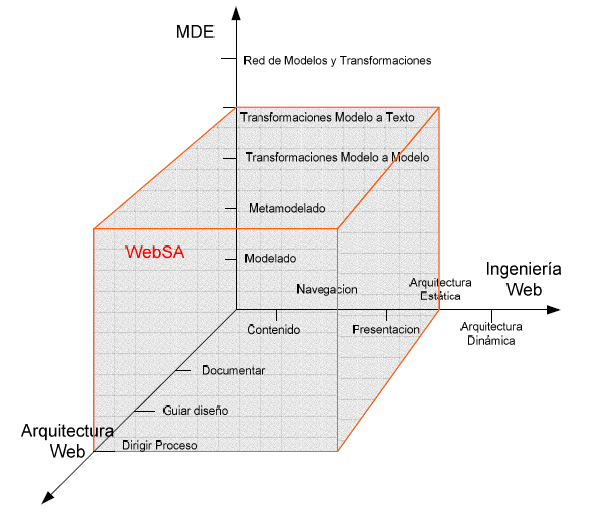
\includegraphics[scale=0.55]{Ch2/f1}
 % arqDHD.: 450x422 pixel, 72dpi, 15.88x14.89 cm, bb=0 0 450 422
\label{fig:planos}
\caption{Área de arqDHD dentro del campo de la arquitectura Web, las metodologías de diseño y su ingeniería} 
\end{center}

\end{figure}


\subsection{Área de construcción de la arqDHD} \label{secc:arqDHD_Situacion}


La Figura \ref{fig:planos} muestra una representación del espacio basada en
tres coordenadas, cada una de las cuáles representa una tendencia: \textbf{Ingeniería
Web} (eje: X), \textbf{Web} (eje: Z) y \textbf{MDE} (eje: Y). Situándose en un estado evolutivo dentro de cada coordenada o tendencia, arqDHD constituye el área dentro de la investigación donde se tomaron las decisiones para su diseño y creación. 

La \textbf{coordenada X} está representada por los conceptos de la Ingeniería Web y en ella se presentan las diferentes vistas que se han ido introduciendo a lo largo de su existencia y cómo las tres vistas funcionales son las primeras en
ser capturadas:
contenido, navegación y presentación. La cuarta vista, también capturada por
arqDHD, es la arquitectura estática. La única vista que no es representada por
arqDHD es la arquitectura dinámica, que representaría el comportamiento tanto
externo como interno de los componentes. Esta tarea no ha sido cubierta por el
presente trabajo.

La \textbf{coordenada Y} es ocupada por la \textbf{Ingeniería Dirigida por Modelos} (MDE) y en
ella se muestran los diferentes estadios por los que ha ido pasando:
representación de las vistas mediante modelos (modelado), formalización de los
modelos mediante el meta-modelado, definición de las transformaciones modelo a
modelo para establecer la traza entre los diferentes modelos del proceso y, por
último, las transformaciones modelo a texto que permiten obtener la
implementación a partir de los modelos.

En arqDHD se construyeron modelos orientados a la conexión de sistemas y artefactos que permitan un correcto ensamblado para lograr los requerimientos y el concepto del requerimiento de inyección de contratos que se viene enunciando. Queda sin embargo un largo
camino de interoperabilidad entre los modelos y transformaciones realizadas, que
permitan establecer una red para compartir los recursos definidos en MDE.


Por último, la \textbf{coordenada Z} la representa la \textbf{Arquitectura Web}. En ella se
muestra una serie de puntos que representan el papel que ha tenido la
arquitectura dentro de las aproximaciones. En un principio la arquitectura
únicamente se utilizaba para documentar. Poco a poco se ha ido extendiendo su
uso como guía para definir el diseño. El último estadio, que es el ocupado por
arqDHD, es aquel en el que la arquitectura define los artefactos más
importantes, dirigiendo el proceso de desarrollo


\section{El contrato como conector}

Entre la diversidad de propuestas de diseño de sistemas e-learning
con características adaptativas, existen diferentes variantes metodológicas y
tecnológicas, una de ellas es la incorporación de contratos context-aware. 

Conceptualizar al contrato como una componente de primera clase, donde las demás
componentes que lo relacionan dependen de su funcionamiento, nos brindará una
visión más completa orientada a la arquitectura y a la conexión entre sus
componentes.
Pensar el contrato como una pieza de conexión (referenciado con el término
“connectors”, conectores, en el área de arquitecturas en ingeniería de software)
nos permitirá incorporar (conectar) nuevos modelos independientes a los llamados framework e-learning.

En la figura \ref{fig:arqDHD1} representamos la integración de un modelo externo con
un framework e-learning por medio de un conector referenciado con el nombre
componente contrato. La componente modelo externo representa una entidad, puede ser un modelo
conceptual, una herramienta, applets, API (Application Programming Interface), o
cualquier sistema independiente que cumpla con la funcionalidad de brindar
información de contexto para ser incorporada en la semántica de la componente
contrato. Las herramientas y los servicios que componen el framework e-learning son
los puntos de comunicación con la componente contrato. Luego, la entidad sistema
representa el ambiente del servidor donde se encuentra el entorno de
la plataforma e-learning.

Este entorno abarca servidores web, servidores de base de datos, sistemas
operativos, archivos y repositorios de recursos, sistemas institucionales, etc.
La mayoría de los clientes deben ser estándares (similares a Web Browsers) y,
las salidas de las aplicaciones deben poder ser presentadas a los clientes
usando lenguaje de marcas tipo HTML.

En el próximo punto, nos centraremos en la importancia del tipo de modelado y
diseño con los que podríamos tratar a los contratos.


\subsubsection{Perspectiva de modelado}

 
El modelado y diseño de sistemas orientados a servicios complejos, no sólo
contribuye a una mejor comprensión de los problemas o posibles soluciones que se
pueden adoptar en un proyecto de I\&D como Obra Abierta, sino que facilita la
comunicación entre el grupo de investigación, especialmente cuando se encuentran
físicamente separados y/o afiliados a diferentes organizaciones.

El trabajo de modelado, es la base de procesos de desarrollo orientados a
servicios para educación y/o investigación, que deben guiar tanto a los
diseñadores como a los desarrolladores en el relevamiento de los requerimientos
pedagógicos y/o investigativos para implementarlos en un artefacto  -objeto- de
software. Esta tarea de modelado puede brindar una guía clara de trabajo al
equipo de I\&D, entregando las soluciones a tiempo y facilitando el logro de un
producto final de alta calidad, con bajos riesgos en el desarrollo.

Atendiendo a los cambios de la tecnología y a la continua evolución de
los estándares, el correcto modelado y diseño de soluciones Web complejas, se
torna cada vez más importante. Resultado de esto, es el nuevo paradigma
de desarrollo en sistemas llamado ”Model-Driver Architecture” (en adelante MDA).

El sistema MDA está focalizado en la importancia de los modelos de
plataformas independientes y plataformas específicas, que permiten una
separación de la abstracción del dominio de conocimiento del particular entorno
de implementación. En la actualidad, dependiendo de los objetivos de
las plataformas, con el desarrollo de herramientas avanzadas para el diseño a
partir de códigos de programación, el rol que cumple el modelo (o
modelado) comienza a ser fundamental. A través del uso de MDA, el modelo
representa a la programación de alto nivel construida para desarrollos de
aplicaciones como, por ejemplo, un dispositivo hipermedial dinámico como el de
Obra Abierta, con requerimientos factibles de trazar (en el sentido del modelado
desde el punto de vista de la Ingeniería de Software). Las herramientas
avanzadas pueden proveer generación automática de código XML, Java u otro código
de programación a partir de un determinado modelo. Un método correcto de
modelado debe brindar el soporte necesario para poder tomar la decisión sobre
qué parte de la aplicación debe ser expuesta como servicio o, qué parte de la
arquitectura debe ser confeccionada para invocar a los servicios Web.


El modelado de soluciones orientadas al servicio no es una tarea simple. Los
servicios heredan algunas características de sus predecesores – objetos y
componentes y también usan elementos del flujo de tareas y de los procesos de
negociación. De esta manera, el modelado de servicios debe cubrir totalmente las
diferentes facetas funcionales y tecnológicas para su prestación
e implementación. El uso de Lenguaje Unificado de Modelado (UML, por sus siglas
en inglés, Unified Modeling Language) como notación semi-formal para el modelado
de servicios es en la actualidad, una elección consensuada por la
comunidad informática.

Aunque en su origen, UML fue concebido para el modelado de sistemas orientados a
objetos, puede ser fácilmente extendido para soportar modelos de otros conceptos
tal como actividades de negocios, interfaces de usuarios y esquema de datos. Sin
embargo, podemos observar que, para el modelado orientado al servicio, todavía
este lenguaje se encuentra en una etapa inicial, ya que no ofrece mecanismos
para la representación de componentes y servicios a nivel lógico.


En Obra Abierta adoptamos estrategias y modelos basados en el concepto de
componentes de servicios que son similares a la propuesta de Zoran (2006), en su
publicación Modeling Services and Components in a Service-Oriented Architecture.
Una componente servicio es un bloque principal que interviene en algún tipo de
relación entre objetos del sistema, las componentes que conforman a los
servicios para educación y/o investigación son modeladas como contratos de
servicios en donde se efectúan algunos de los procedimientos pedagógicos o
investigativos (en forma de reglas) como ejecuciones de operaciones entre los
objetos.


El concepto de la componente contrato ha sido introducido en el capítulo
anterior, como una pieza de software que permitía la adaptación de servicios al
contexto de los objetos que lo utilizaban, o sea como componente para establecer
algún tipo de relación “controlada” entre ellos. En este capítulo, a los
contratos los abordaremos desde la perspectiva de los MDA, haciendo referencia
al propio modelo adoptado en Obra Abierta.


\subsection{Los conectores en entornos adaptativos}


\Section{Aspecto Dinámicos de la Arquitectura DHD}

Dichos sistemas son altamente dinámicos y muestran una estructura evolutiva.
Continuamente se añaden, eliminan o se reemplazan componentes, a veces incluso
como parte del funcionamiento normal. Estos detalles ya no son coyunturales,
sino estructurales y deben tenerse en cuenta durante el Diseño del sistema.
Por lo tanto, para ser realmente útil, un Lenguaje de Descripción de Arquitectura
(Adl) debe ser capaz de especificarlos. Sin embargo, esto no es lo normal en los
Adls existentes, cuya naturaleza es mayoritariamente estática. Los pocos que
muestran capacidades dinámicas muestran también limitaciones, que dependen en
gran medida de sus orígenes particulares.

Cuando la evolución de una arquitectura es continua y los cambios en su
interior siguen un patrón predefinido, entonces ha de considerarse que este
patrón forma parte intrínseca de la estructura. El objetivo de la Arquitectura
de Software es describir la estructura de los sistemas y, esto debería incluir
tanto a sus partes fijas o estáticas, como las partes cambiantes o dinámicas. De
hecho, en muchos sistemas, el rasgo diferencial, que lo distingue de otros
sistemas similares es el comportamiento dinámico de su arquitectura ya que a menudo,
puede resultar aún más importante que el esquema estático de partida. Algunos
ejemplos de sistemas para los que la definición de dinamismo es esencial son
los siguientes:

\begin{itemize}
 \item Los sistemas abiertos y distribuidos, cuya estructura cambia de manera
constante.

\item Los sistemas evolutivos de varias clases, que se ajustan a un cierto
patrón.

\item Los sistemas multi-agente (MAS), dentro y fuera del contexto
de Inteligencia Artificial y en general todos los sistemas capaces de expresar 
algún grado de movilidad.

\item Los sistemas reflexivos, que son interesantes en sí
mismos, pero que, además, constituyen la base de la propuesta final de este
trabajo.

\item Los sistemas continuos, de tiempo real y tolerantes a fallos, en los que
a menudo se requieren cambios, pero que no pueden ser detenidos para ser
actualizados.

\item Los sistemas adaptativos o auto-organizados, que modifican su propia
estructura para adaptarla a cada entorno concreto.

\end{itemize}


El DHD es parte de la última familia de sistemas enumerados, donde se permite
a través de una característica arquitectónica poder resolver requerimientos
funcionales, en este caso de adaptación, mediante la conjunción (conexión)
coordinada de subsistemas.


Hoy en día, todas estas propuestas han sido desarrolladas, y muchas otras se
han ido incorporando; muchos sistemas anteriores han sido adaptados o
reconocidos como Adls dinámicos, y se han desarrollado varias tesis doctorales
en todo el mundo [Cra97, MG99, Med99, dP99, Sch99, Wer99,Pry00, CV00] dedicadas
a este tema de algún modo. En definitiva, el desarrollo e interés creciente
de este campo es innegable, y se presenta, sin duda alguna, como uno de las
líneas de trabajo más fructíferas de la próxima década.


\section{Tipos de Dinamismo}

Todo sistema de software cuya estructura es descripta como una arquitectura tiene
siempre asociado algún tipo de comportamiento dinámico. Ahora bien, es
obvio que este dinamismo no siempre indica el mismo grado de variabilidad.
Algunos sistemas muestran una estructura inalterable, en la que los distintos
elementos se limitan a comunicarse. Otros sistemas, en cambio, muestran una topología interna que se altera continuamente e incluso se incorporan nuevos tipos de elementos.

Resulta fundamental, para poder realizar una comparación adecuada entre las
distintas aproximaciones, delimitar los diferentes tipos de dinamismo que
pueden aparecer en un sistema software.

La clasificación que se incluye más abajo ha sido planteada con este único
objetivo. No es exacta, ni pretende ser determinante ya que el límite entre las
distintas categorías puede aparecer difuminado en algunos casos. Sin
embargo, parece servir adecuadamente a su objetivo, esto es,
aclarar el tipo de actividad al que se hace referencia en cada casoy que ha
sido publicada en dos ocasiones [CFBSB00, CFBSB01].

Según esto, entonces, pueden identificarse los siguientes tres tipos de
dinamismo, en orden creciente de potencial para el cambio:

\begin{itemize}
\item 
Dinamismo Interactivo. Este término se refiere al movimiento de datos
entre componentes, el dinamismo inherente en la comunicación e interacción
usual. Se relaciona con cuestiones tales como la sincronización y los
protocolos afectando no solo a la estructura sino, también, al comportamiento de un sistema
computacional. Está presente de manera implícita en todo sistema, pero resulta
particularmente obvio en los concurrentes y paralelos.

\item
Dinamismo Estructural. Hace referencia a los cambios que afectan a los propios
componentes y sus interacciones, que normalmente se expresan como la creación
y destrucción de instancias y enlaces entre componentes. En este sentido, la
arquitectura de software del sistema resulta alterada, porque lo que cambia es
la estructura. Este tipo de dinamismo es natural en sistemas distribuidos.


\item 
Dinamismo Arquitectónico. Se refiere a los cambios en los tipos de
componente e interacción, modificando por lo tanto incluso el significado y el 
“vocabulario” del sistema. Se expresa como la inserción de nuevos tipos de
componente (y conector) y el borrado de algunos ya existentes. Ahora, lo que
cambia es la infraestructura, el sustrato en el que las arquitecturas se
definen, su meta-nivel. Este es el nivel definitivo de dinamismo y también el
más difícil de capturar y utilizar. Aún hay que demostrar su verdadera
importancia y utilidad, pero está claramente presente en los (auténticos)
sistemas abiertos.

\end{itemize}
\subsection{Reconfiguración Dinámica}

Hay al menos dos aproximaciones a la especificación de dinamismo en sistemas de
software. Una de ellas trata de encontrar un conjunto adecuado de comandos
imperativos, capaces de expresar cualquier configuración deseable. La otra
utiliza una sintaxis declarativa, que es generalmente más potente e intuitiva,
pero que no siempre tiene la flexibilidad deseada. El trabajo sobre este tema
se centró inicialmente en el primer enfoque; sin embargo, a medida que se
alcanza una mejor comprensión del dinamismo estructural, la presencia del
segundo tiende a aumentar.

A menudo, la denominación Arquitectura de Software Dinámica (ASD) ha sido
discutida. Muchos autores prefieren el término Reconfiguración Dinámica, que
ha sido consagrado por años de trabajo previo en el campo específico de la
configuración de sistemas distribuidos. Con esa expresión se hace referencia,
en general, a los cambios producidos en la topología de un sistema compuesto, igual a decir a cualquier alteración en el número y orden de los nodos y
los enlaces que lo constituyen. Lo cual es equivalente al grado de dinamismo que actualmente se
está alcanzando en los Lenguajes de Descripción de Arquitecturas. Según Jeff
Kramer, el nombre de Arquitectura Dinámica debería reservarse para referirse a
los sistemas en los que incluso el tipo de componentes implicados puede cambiar.
Este es, precisamente, el nivel de descripción al que se pretende llegar, por
lo que a lo largo de este trabajo esa expresión será utilizada a menudo, sin
mayores consecuencias.


\subsection{Tipos de Reconfiguración}

Hay varios tipos distintos de reconfiguraciones posibles, que manifiestan
problemáticas muy diferentes. Con el fin de determinarlas con mayor exactitud,
se han introducido una serie de clasificaciones. En este trabajo se mencionarán
dos de ellas, a saber:

\begin{itemize}
 
\item Según el tiempo. Uno de los aspectos críticos en un cambio es el
momento en que se produzca. La dificultad para realizarlo de manera adecuada
crece según se avanza en el proceso de desarrollo.

\begin{itemize}
\item Antes de la Compilación. Los cambios en la estructura prevista del
sistema se producen antes de su construcción, por lo que sólo hay que asegurar
su consistencia.

\item Antes de la Ejecución. El sistema ya ha sido elaborado, pero aún no
está funcionando, por lo que introducir un cambio sólo requiere, de nuevo,
asegurar la consistencia interna del sistema. Puede equipararse sin problemas
con el caso anterior.

\item Durante la Ejecución. Esta última es la auténtica Reconfiguración
Dinámica ya que los cambios se producen con el sistema en marcha: los componentes
tienen un estado y sus enlaces soportan cierto número de transacciones. La
problemática generada por este tipo de situaciones ha sido el campo de
investigación de la comunidad de configuración en los últimos diez años.
\end{itemize}

\item Según el origen. Es decir, según cómo se inicie el proceso y de acuerdo a quién tome la iniciativa, existen dos posibilidades que son las
que se detallan a continuación: 

\begin{itemize}

 \item Reconfiguración Programada. Reciben este nombre [EW92, MG99] las
operaciones que son iniciadas por el propio sistema, mediante una serie de
reglas proporcionadas como parte de su especificación. También, se ha mencionado
como reconfiguración restringida en tiempo de ejecución [Ore96], y es el
nivel de descripción que se desea alcanzar en la Arquitectura de Software.

\item Reconfiguración Ad-Hoc. Además de este nombre [EW92], ha recibido los
de reconfiguración evolutiva [MG99] o en tiempo de ejecución [Ore96]1. Hace
referencia a los cambios que son introducidos manualmente por el usuario y que,
por tanto, requieren en concurso de algún tipo de herramienta que haga
corresponderse a la arquitectura con un sistema real. Obviamente, no pueden ser
previstos, aunque en general sí pueden ser controlados.

\end{itemize}

\end{itemize}


La primera clasificación es obvia y ha sido planteada, entre otros, como autores del nivel de Wermelinger [Wer99]. La segunda clasificación, se debe inicialmente a los trabajos de Markus
Endler en Gerel [EW92], un lenguaje ligado a δarwin, pero que ha sido redescubierta
en múltiples ocasiones por otros autores; lo cual explica la gran variedad de
terminologías utilizadas.


\subsection{Operaciones Básicas de Reconfiguración}

Desde casi el principio, se ha determinado que toda configuración ha de poder
ser descripta en función de cuatro operaciones básicas, cuyo establecimiento
procede de Conic (§3.6.1). En realidad, no es muy difícil deducirlas de la
simple observación de un grafo, considerando en este caso al grafo como la
descripción más simple posible de la topología de cualquier sistema, en la
que los componentes se expresan como nodos y sus enlaces como aristas.

Las cuatro operaciones mencionadas son las siguientes:

\begin{itemize}

\item 
Crear (create). Se refiere a la creación de nuevos componentes.  Para ser
exacto, la instanciación de un nuevo ejemplar de un tipo de componente conocido. 

\item
Destruir (destroy). La inversa de la anterior: permite destruir un
componente ya
existente, eliminarlo del sistema.

\item
Enlazar (link). Crea un enlace simple entre dos elementos.

\item 
Desligar (unlink). La inversa de la anterior: destruye un enlace
preexistente.

\end{itemize}

Es importante aclarar que las ideas previas no significan que todo sistema de reconfiguración haya de tener
estas cuatro operaciones indicadas de manera explícita; al contrario, muchos
las expresan mediante estructuras declarativas y ni siquiera tienen
un equivalente claro para algunas de ellas. Lo que sí debe quedar claro es que toda reconfiguración, por compleja que sea, puede realizarse     
mediante la aplicación sucesiva de estas cuatro operaciones. Del mismo modo, si
un sistema no es capaz de expresar una transformación que, sin embargo, puede
ser descripta en función de estas cuatro operaciones, entonces puede afirmarse que el sistema no es
completo en lo que respecta a este tema. 

En realidad, estas operaciones proporcionan lo que aquí se ha denominado con el nombre de Dinamismo Estructural ya que, únicamente, permiten alterar la topología
del sistema. Sin embargo, constituyen lo que podría considerarse el límite
mínimo exigible a cualquier sistema que pretenda expresar arquitecturas
dinámicas. 

En los DHD el dinamismo está basado en la operación denominada Enlazar
(link). No obstante, a lo largo de la revisión podrá verse que hay dos
modelos conceptuales que predominan claramente por sobre cualquier otro; esto, no solamente es
cierto en los Adls dinámicos sino incluso en los más convencionales. 



\section{Descripción arquitectónica de los DHD} \label{secc:arqDHD}



En esta sección se presenta el modelo de arquitectura denominado arqDHD con un diseño adecuado para la implementación, configuración y posibles cambios en los procesos de inyección de contratos sensibles al contexto en entornos de eLearning originales (EeLO) \label{EeLO}. En la principal decisión de diseño se tuvieron en cuenta las atribuciones dinámicas que se persiguen y se seleccionaron cuáles serían los lugares apropiados para incorporar el ContratoDHD. 


\begin{figure}
\begin{center}
 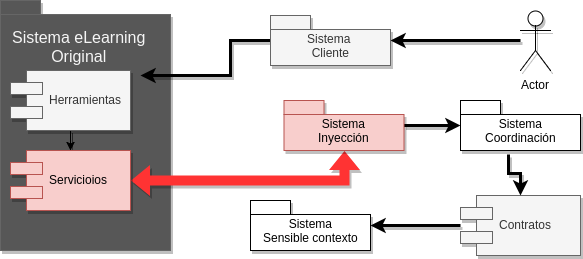
\includegraphics[scale=0.55]{Ch2/ArqDHD2.png}
\caption{Elementos arquitectónico involucrados en el proceso de inyección} \label{fig:arqDHD1}
\end{center}
\end{figure} 


La figura \ref{fig:arqDHD1} representa los elementos y las relaciones de una arquitectura que se tuvieron en cuenta. Por un lado, se parte de un sistema eLearning original reducido con las componentes “herramientas” donde se engloba la representación de todas las herramientas colaborativas (por ejemplo  una wiki, un foro, un examen, diversos recursos hipermediales, etcétera) que una determinada plataforma eLearning puede ofrecer a los usuarios finales. A su vez, se relaciona con la componente “servicio” encargada de representar las implementaciones de los métodos (funcionalidades) que ofrecen las herramientas que eventualmente pueden ser compartidas por varias de ellas (por ejemplo editar, consultar, publicar, borrar, aceptar, etcétera). Este tipo de relaciones es típico de los sistemas colaborativos web, manteniéndose como un estándar para este dominio de aplicaciones. 

Los otros elementos que aparecen en la arquitectura son dos sistemas que tienen relación directa con el sistema original. El primero es una representación para cualquier tipo de mecanismo de comunicación con las herramientas, particularmente en el framework Sakai \cite{sakaimanual} que estarían, a su vez, representadas las capas Presentación, Agregación y Clientes. El otro sistema conectado tendrá la responsabilidad de efectuar la inyección de los contratos sensibles al contexto. Esta relación está indicada con una flecha roja bidireccional para señalar que hay un importante flujo de mensajes de entrada y salida sobre la componente servicio. De esta manera, queda establecida un bloque de inyección entre la capa servicio, el subsistema de inyección y la relación bidireccional entre ellos. Entonces, la inyección se produce modificando únicamente la capa de servicio del framework original. En los capítulos que a continuación se presenta el desarrollo, se brindarán los detalles de diseño e implementación para esta relación.

Por otro lado, el sistema de inyección será el encargado de relacionarse con el sistema de coordinación de contratos que tiene la tarea de asegurar las propiedades dinámicas a la arquitectura. Específicamente, aquí se producen los reemplazos de contratos, a través de una nueva relación con el componente arquitectónico denominado \textbf{Contrato}, en el tiempo de ejecución configura el primer grado de adaptabilidad del sistema desde la arquitectura. La última relación, está dada entre el contrato y el sistema \textbf{Sistema Sensible al contexto} que se encargará de ofrecer la infraestructura necesaria para transformar al contrato en contrato sensible al contexto del DHD (ContextoDHD \ref{ContratoDHD}). 




\subsection{Diseño para la inyección}

En la publicación denominada \textit{" Investigación en el diseño y desarrollo para el enriquecimiento de
Un framework colaborativo web sensible al contexto "} (Sartorio et. al) \cite{inyecccion} aparecen los avances consolidados en el estudio-aplicación-desarrollo
de los aspectos fundamentales para el enriquecimiento de un framework web colaborativo con propiedades de sensibilidad al contexto
(FWCsc). Para este propósito se definió una estrategia y, en la presente sección, se expondrán los secretos de implementación y decisiones de diseños, que incluyó las siguientes acciones: 

Primero, desarrollando tareas de diseño, testing, documentación
de estilos arquitectónicos y especificación de una herramienta colaborativa web, teniendo en cuenta técnicas y metodología de desarrollo actuales. Segundo, implementación, instalación, configuración y soporte de una aplicación utilizando frameworks de desarrollo estándares. Tercero, consolidar ambientes y prácticas para el aprendizaje-enseñanza-investigación, colaboración y otros usos (compartir experiencia, vinculación con la comunidad de usuarios con intereses similares, K-12, Higher-Ed, Portfolios), en la construcción de espacios colaborativos web sensibles al contexto.

\subsubsection{Enfoque partiendo de Framework e-learnig originales}

La implementación de plataformas colaborativas constituye unos
de los medios más versátiles para el uso en actividades académicas. Un ejemplo que puede ser citado de este tipo de aplicaciones son: 
WebCT, BlackBoard, e-ducativa, Plataforma Mediáfora, Dokeos,
OfficeManager, Moodle, Nexus, ILIAS, Claroline.

Su constante evolución, crecimiento y adaptación permiten
tener cada vez mejores prestaciones y servicios. El eficiente uso
de estas plataformas implican tener sólidos conocimientos técnicos
para su instalación, mantenimiento y desarrollo. Al mismo tiempo
se debe contar con mı́nimas habilidades para la creación de los
distintos espacios de trabajos y definir las metodologı́as de uso.


En el marco de los análisis efectuados y teniendo en cuenta
experiencias de nuestro grupo de trabajo se sostiene que la incursión en
proyectos “open source“ con gran aceptación científica brinda una
de las propuestas más consolidadas de diseño y desarrollo de entornos colaborativos Web para educación, orientado a herramientas que se implementan a través de servicios comunes (denominados servicios bases). Por ejemplo, existen frameworks orientados a portales
donde el servicio de edición de mensajes es utilizado en herramientas tales como Foro, Anuncio, Blog, etcétera. Más aún, otra de las características salientes es la versatilidad para su extensión y/o configuración. En efecto, es posible alterar ciertas configuraciones
en tiempo de ejecución, por ejemplo, instrumentar una nueva funcionalidad en un servicio base.

Para este propósito se iniciaron estudios sobre la arquitectura y el diseño a partir de infraestructuras de aplicaciones e-Learning para la construcción y estudios de mejores técnicas de Especificación, Diseño, Modelado, Testing, Formalización y Documentación como aportes en el campo de la Ingenierı́a de Software. Además, es necesario definir y documentar adecuadamente el camino de construcción hacia  aplicaciones Web basadas en un framework colaborativo, con propiedades de sensibilidad al contexto y la utilización de contratos \cite{arqDHD21}



\susubsection{Punto de partida}

Los avances en las principales comunidades cientı́ficas sobre desarrollos de herramientas Web colaborativas permiten la participación
en varios niveles dentro de una activa comunidad de educadores, referentes institucionales y desarrolladores inspirados en las actividades de enseñanza, aprendizaje e investigación. Particularmente, los diseñadores y desarrolladores del proyecto Sakai \footnote{https://sakaiprojecto.org} trabajan conjuntamente con docentes y estudiantes profesionales de universidades internacionales. En este sentido, algunas de las universidades involucradas
en este proyecto son: Indiana University, University of Michigan, Yale University, Stanford University, Universidad Politécnica de Valencia y la Universidad del Valle de Guatemala. Todas ellas promueven la disminución de las distancias entre las necesidades del usuario final y el software. Ahora bien, debemos destacar que el mayor flujo de las actividades colaborativas se concentran en la lista de “e-mails”, “wiki”, “foros”, etc. Los miembros de estas comunidades presentan todo tipo de perfiles académicos e institucionales.


\begin{figure}
\begin{center}
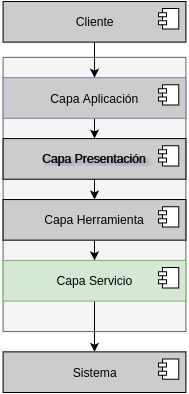
\includegraphics[width=2.5 in,totalheight=3 in]{Ch2/felo.png}
\caption{Elementos arquitectónico involucrados en el proceso de inyección} \label{fig:FeLO}
\end{center}
\end{figure} 


El punto de partida de esta experiencia se inicia con un diseño de arquitectura conceptual genérica a las que se ajustan los framework eLearning más populares. Luego, se identificarán los extractos de la arquitectura donde se representan los servicios de las herramientas. Se continúa con una propuesta de diseño que permita implementar el concepto de inyección referido en la sección \ref{secc:arqDHD}. Por último, se añaden nuevas componentes importantes de la arquitectura que complementan los aspectos adaptativos de los contratosDHD.  


El primer agregado al sistema web colaborativo original se produce a niveles de capas. El Framework Sakai está diseñado según una arquitectura de cuatro estratos de capas representada en la figura \ref{fig:FeLO}

La capa de \textbf{Agregación}, tiene la responsabilidad de las salidas de Sakai (y también aplicaciones externas a Sakai) que pueden ser combinadas utilizando una aplicación Servidor alojada aquí. Contiene un gestor de pantalla donde se controlan sus estados reales y ciertas transacciones de interfaz de usuario. Los soportes de accesibilidad son provistos por una combinación de interfaces de usuarios estándares esta capa y la de presentación.

La capa de \textbf{Presentación}, encargada de combinar los datos que provienen de las herramientas Sakai y las interfaces de usuarios creando metadatos al contenido que se brinda a los usuarios. Esta información es persistida externamente y será utilizada para poder analizar todas las experiencias a través de una herramienta Sakai denominada registro de actividades.  

La capa \textbf{Herramientas}, concentra la estructura de contenedores donde se encuentran la lógica de las funcionalidades que proveen las herramientas Sakai implementadas en los servicios y, también, las conexiones con la capa de presentación. Las herramientas atienden los pedidos de los usuarios y las respuestas a eventos del entorno, luego remite a los servicios adecuados y se encarga de proporcionar la respuesta a la capa superior.


La capa \textbf{Servicios}, interpreta a los servicios como una colección de clases que transforman datos para definir comportamientos. Estos datos pueden tener representaciones internas o ajustarse a los estándares de la comunidad industrial y/o científica. Las funcionalidades también pueden ser provistas a través de interfaces de aplicaciones (API). Un servicio puede invocar a otro servicio y creando dependencias. Los servicios son modulables y se ajustan a un diseño apropiado con el propósito de ser reusables y portables.

En los  capítulos precedentes se explicaron algunos de los fundamentos sobre el diseño de arquitectura a nivel arquitectónico. En esta sección de la investigación doctoral, se retoma la idea de inyección explicada anteriormente a nivel de arquitectura. Ahora, se propone un diseño para envolver los servicios del núcleo Sakai para el mecanismo de coordinación de contratos. De esta manera, se altera el diseño original del framework, agregando y modificando componentes que permitirán una mejor representación respecto a la inyección de información de contexto y el agregado de una nueva pieza de software que posee propiedades de sensibilidad al contexto mencionadas. Con este propósito, fue modificado el diseño de la capa de servicios original \cite{arqDHD17}, mediante una división en tres partes:


\begin{figure}
\begin{center}
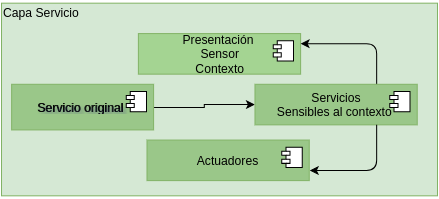
\includegraphics[scale=0.55]{Ch2/CapaServicio.png}
\caption{Elementos arquitectónico involucrados en el proceso de inyección} \label{fig:CapaServicio}
\end{center}
\end{figure} 



\begin{itemize}

\item \textbf{Servicios Originales:} Pertenecientes al núcleo del framework original, no afectados con el agregado del mecanismo
de coordinación de contrato.

\item \textbf{Servicios de Contexto:} Permite a clientes el acceso a en-
tidades, asignar, obtener y subscribir cambios en la información de contexto de las entidades.

\item \textbf{Servicios con coordinación de contratos (Servicios CSC):}
Servicios base del núcleo del framework Sakai modifica-
dos para poder efectuar la envoltura de los mecanismos de
coordinación.


\end{itemize}

Mediante la división del estrato servicios se puede interpretar a
los Servicios CSC como una nueva arquitectura basada en sistemas
estratificados[11]. Entonces, esta composición se efectúa por el estrato de coordinación de contratos y el estrato de cómputo. La capa
de cómputo estará compuesta por módulos de implementación (como por ejemplo los 
servicios Sakai previos a la incorporación de contratos). Mientras que la capa de coordinación estará compuesta por módulos
especı́ficos de coordinación, patrones tipo proxy y contratos.
La implementación de los Servicios CSC se realizarán utilizando un patrón de diseño de coordinación de contratos (”Coordination Contracts Design Pattern”) tomando como referencia
la propuesta de Fiadeiro \cite{arqDHD12, \cite{arqDHD13}. Este patrón está basado en el
patrón de diseño ”proxy” (o “Surrogate“) \cite{arqDHD14}. Por un lado, provee
una interfaz especı́fica (“SubjectInterface“), como una clase abstracta, para cada componente. Esta interfaz está conectada al programa real (”SubjectBody”) a través de un proxy dinámico reconfigurable. Por otra parte, soporta la reconfiguración dinámica del
código ejecutado por medio de solicitud de operaciones a través
del “proxy”.

El segundo subsistema está compuesto por una componente
contrato y su correspondiente mecanismo de coordinación. En este
caso, la coordinación del contrato se define como:
En términos generales, la coordinación de contratos es una
conexión establecida entre un grupo de objetos (en nuestras consideraciones los participantes serı́an un objeto cliente y un determinado servicio), donde reglas, normas y restricciones (RNR) son


\begin{comment}

\begin{figure}
\begin{center}
 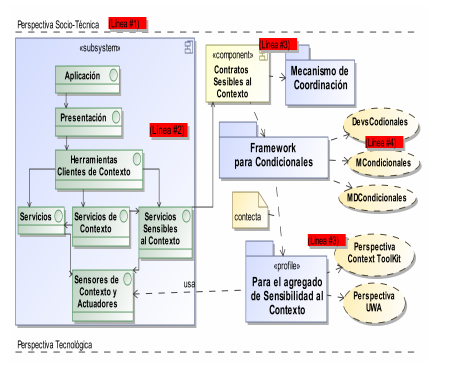
\includegraphics[scale=0.55]{Ch2/arqDHD_Implementacion.png}
 \caption{Arquitectura conceptual del DHD} \label{fig:arqDHD2}
\end{center}
\end{figure}

\end{comment}





superpuestas entre los actores participantes, estableciendo con un
determinado grado de control las formas de interrelación (o interacción).

El tipo de interacciones establecidas entre las partes es más
satisfactoria que las que se pueden lograr con UML o lenguajes
similares (orientados a objetos) debido a que éstas contienen un
mecanismo de superposición en el que se toman como argumento los
contextos. Cuando un objeto cliente efectúa una llamada a un objeto suministro, 
el contrato ”`intercepta”  la llamada y establece una
nueva relación teniendo en cuenta el contexto del objeto cliente, el
del objeto servidor e información relevante (respecto de la relación)
adquirida y representada como contexto del entorno. Como condición
necesaria, la implementación de los contratos no debe alterar el
diseño y funcionalidad en la implementación de los objetos.


El tercer subsistema corresponde a un framework implementativo “contex-awareness” que permite integrarse con algunas de las
componentes del primer subsistema para la recolección del censado de información de contexto. Luego, dicha información es
procesada a través de mecanismos que permitirán incorporarles
propiedades de sensibilidad al contexto. Su configuración fue resuelta a partir de las ideas fundadoras del trabajo de Dey sobre el
Context ToolKit \cite{arqDHD15} y el proyecto UWA \cite{arqDHD16}.

El cuarto subsistema lo compone un nuevo modelo pensado
para el diseño e implementación de condicionales que puedan ser
utilizados en la composición de reglas de contratos. La principal
idea de esta propuesta es estandarizar soluciones y brindar información necesaria en la creación de condicionales, donde su valores
de verdad deban se calculados a través de sistemas externos, como por
ejemplo, el tercer subsistema de la figura1. En este sentido,
los tipos de condicionales serán abstraı́dos en modelos que com-
prendan cálculos a partir de métricas, estructuras y simulación de
eventos discretos. También, puede verse a este subsistema como
integrador (conector) entre el subsistema de coordinación de con-
trato (segundo subsistema) y el sensible al contexto (tercer subsis-
tema).



\subsubsection{Áreas de integración}


A partir de \textbf{arqDHD} se comienzan a ordenar las cuestiones de diseños e implementaciones abordados en los siguientes capítulos. A lo largo de este recorrido se harán referencias directas e indirectas a todos los conceptos y enfoques abordadas en este capítulo. A su vez, se pueden identificar cuatro enfoques de interpretación y utilización de arqDHD. Cada una está relacionada con un conjunto de los elementos, relaciones y propiedades (de elementos y relaciones) de arqDHD. A continuación, se brindará una descripción conceptual que ponga en evidencia otros de los aspectos estructurales de nuestra propuesta de inyección de contratosDHD.


\begin{figure}
\begin{center}
 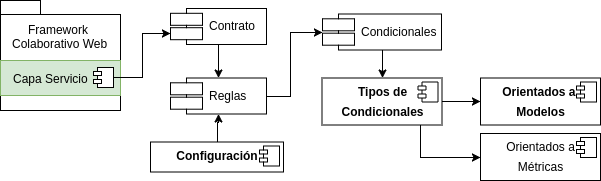
\includegraphics[scale=0.55]{Ch2/arqAreas.png}
 \caption{Áreas } \label{fig:arqAreas}
\end{center}
\end{figure}



Así como la arquitectura de la figura \ref{fig:arqDHD1} tiene definido los sistemas necesarios para la inyección, también fue necesaria definir áreas de integración en las que se pueda trabajar con herramientas y recursos externos en módulos para poder hacer incorporarlos de forma directa y con el menor costo de diseño e implementación posible. A continuación, se describen estas áreas con sus aportes para \textbf{arqDHD}.

\begin{enumerate}

\item \textbf{Área del estudio de arqDHD}
 
Este capítulo está dedicado a una propuesta de arquitectura para el DHD donde se tiene en cuenta varios aspectos arquitectónicos de los Framework eLearning originales y todos los elementos que intervienen en el proceso de inyección de los contratos. Principalmente, se tuvo en cuenta elementos, relaciones y las propiedades con alto impacto en el desarrollo e implementación. Para este propósito, se realizaron estudio de adaptación y aplicación de documentación de estilos arquitectónicos al framework web colaborativo Sakai con contratos sensibles al contexto \cite{arqDHD21}. Se proporcionan diferentes formas de interpretar la arquitectura Sakai con el propósito de construir una documentación adecuada a su comunidad de desarrollo \cite{arqDHD18}.

Luego, se propone una arquitectura ideal que describa la incorporación de contratos sensibles al contexto(CSC) utilizando estilos arquitectónicos y patrones de diseño. También, se persigue el propósito del agregado de propiedades de adaptación dinámica a los servicios bases del Framework Sakai. El esquema de la figura \ref{fig:arqAreas} define un mapa conceptual de las disposición de los elementos principales que se tuevieron en cuenta en la áreas denominada: ”Área del estudio de arquitectura y definiciones de arqDHD”. 


\item \textbf{Área de estudio de configuración de reglas de contratosDHD}
 
 
La configuración de las reglas de los contratos es una cuestión relevante para lograr adaptabilidad. Por este motivo, se tomaron como referencia obligada los trabajos de prueba de campo realizados en la tesis de la Dra. Soledad Ayala \cite{tesis:Soledad2014} quien analiza, desde una perspectiva socio-técnica, cómo se construyen las prácticas de lectura en el nivel educativo superior a través del uso de materiales educativos adaptados al \textbf{FWCsc}. A partir de los resultados de dicha investigación doctoral, obtuvieron protocolos e información necesaria para la construcción de reglas de contratos teniendo en cuenta diversos usos de las tecnologı́as considerando la compleja relación entre los aspectos sociales (de índole idiomática, cultural, educativa, legal, entre otros) y los aspectos técnicos de cada uno de los artefactos en particular y de los software en general.

Esto posibilitó ver cómo cada una de las distintas funciones
internas de las \textbf{FWCsc} se interrelacionan entre sı́, pero, principalmente, pensarlas en congruencia con la utilidad que los usuarios pueden otorgarles. En este sentido, la Dra. Ayala se pregunta acerca de cómo pueden identificarse y conceptualizarse los usos las tecnologías digitales desde un punto de vista epistemológico relativista de la tecnología. No hay un solo uso o un uso “correcto”, sino que coexisten usos adecuados, múltiples, correctos, orientados hacia ciertos fines, según el modo y los significados atribuidos por cada usuario. Cualquiera que estos sean, lo relevante de esta perspectiva es que permite analizar el vínculo entre los procesos de diseño y producción de las tecnologías y los diferentes usos que de los software, pero, además, posibilita al investigador interrogarse sobre los rasgos actuales que predominan en los usos referidos a las tecnologías digitales, el modo en que están siendo pensados, cómo se llevan a cabo, cuál es el estado de la cuestión y cuáles son los desafı́os presentes y futuros. 
El ámbito educativo es solo una arista fundamental de un campo que ya demostró en el desarrollo del hardware que el cielo es el lı́mite. Ahora bien, el análisis de los múltiples usos que realizan los diversos usuarios del otro lado de la pantalla”, del “cómo” los usuarios recuperan el diseño  y la arquitectura del programa, es uno de los mayores desafíos en las investigaciones referidas a la arquitectura de software. Queda por delante un desafı́o casi inacabable: recobrar la mirada del usuario, sus objetivos, pero por sobre todo, su forma de relación con la tecnologı́a y los rasgos de los procesos de interacción que co-construye con cada uno de los sistemas con los que interactúa, cualquiera que éstos sean. 


\item \textbf{Área de estudio sobre los condicionales.}

Esta área de estudio tiene el propósito de brindar un marco conceptual sobre la posibilidad de creación e implementación de condicionales adaptables al diseño y
propósito de los contratos sensibles al contexto. En la figura \ref{fig:arqAreas} está representado por las componentes \textbf{Condicionales} y su relación con \textbf{Reglas}.

En este caso, se propone un modelo de integración para conectar un subsistema que colabore con la configuración (cálculo) de los valores de verdad de las reglas de los contratos \cite{arqDHD19, arqDHD21}. Para este fin, se abordan líneas temáticas relacionadas con patrones de diseño, diseño de módulos y arquitectura de
software. Además, se plantean aspectos relacionados con la creación de metodologı́a y documentación específicas.

La figura \ref{fig:arqDHD2} representa una idea de la propuesta de diseño basada en los módulos que se deben tener en cuenta para concretar un diseño eficiente de  condicionales. En este caso, a partir de un módulo de integración \cite{arqDHD2} se concentran el control de las partes intervinientes. De esta manera, se define un módulo donde se efectúan los cálculos finales que determinan el valor de verdad del condicional.
Otro módulo es encargado de la recolección y toma de datos, extendiéndose para los casos particulares donde sea necesario contar con estructuras de árboles (como por ejemplo MDCondicionales \cite{arqDHD20}), aplicación de métricas (como por ejemplo MCondicionales \cite{arqDHD20}), expresiones lógicas, entre otras. Además, un módulo aparte se configura para describir todas las restricciones que deben cumplir el condicional, teniendo en cuenta su utilización dentro de las reglas de los contratos, con el propósito de no incurrir en contradicciones o inconsistencias con las “pre” y las “post” condiciones e invariantes. Las conexiones con otros subsistemas, por ejemplo, el sub- sistema sensible al contexto representado en la figura1, se encuentran encapsuladas en otro módulo de conexión. De esta manera, se implementa un  “callback” de un método perteneciente a la interfaz de un subsistema externo.

\item \textbf{Área de desarrollo e implementación de métricas para el análisis de las interacciones para el FWCsc}

En esta lı́nea se propone el desarrollo e implementación
de mejoras en las métricas para el análisis evaluativo de
la calidad de las interacciones en redes sociotécnicas mediadas por los \textbf{FWCsc} para la construcción y diseminación de conocimiento \cite{arqDHD1}. Estas métricas cuantitativas y cualitativas, son flexibles a los diversos requerimientos, tanto de los sujetos participantes como de las tecnologı́as sociales y digitales y se exponen atendiendo al marco teórico y metodológico de los Dispositivos Hipermediales Dinámicos\cite{arqDHD20}. En la figura \ref{fig:arqDHD} la componentes denominada \textbf{Orientados a Métrica} y \textbf{Tipos de Condicionales} establecen las estructuras que permitirán poder diseñar y construir condicionalesDHD donde sus grados de valor puedan ser inferidos a través de una métrica. Para este propósito, en los capítulos siguientes se presentará un diseño de aplicación de métricas a los contratos y, en particular, aplicaremos un tipo de condicional que deviene de la teoría de sistema complejo utilizando el formalismo DEVS (Discrete EVents dynamic Systems) para su modelado global y la integración tecnológica de dichas métricas.
También, sumamos el resultado obtenido en un caso de uso utilizando el entorno PowerDEVS. Así, la propuesta sienta las bases para el desarrollo de una herramienta de seguimiento
de procesos participativos que tienen como objetivo educar, investigar, producir y gestionar. A su vez, se obtiene un indicador para el cambio contextual de los participantes, resignificando una de las característica de sus comportamientos y atendiendo a la posibilidad de usar la información de interactividad como parámetro  “context-aware”  de los contratos. Al mismo tiempo, se consideró la posibilidad de establecer interfaces de conexión para ser utilizada como parte del cálculo de los valores de verdad de condicionales de las reglas en los contratos sensibles al contexto \cite{arqDHD2}.



\section{Conclusiones}

completar ...




% -- Archivo Cap\'{\i}tulo N� 3 --
%%-------------------------------------------------------------------------------------------------------------
%------------------------------------------------- Chapter 3 -------------------------------------------------
\chapter{Models and Architectures}
\pagenumbering{arabic}

\section{Introduction}

This chapter describe the fundamentals aspecto an dicisions 

\section{Models}
\subsection{Context Model}
\subsubsection{Key-Value Models}
\subsubsection{Markup Sheme Models}
\subsection{Graphical Models}
\subsubsection{Object Oriented Models}
\subsection{Logic Based Models}
\subsection{Ontology Based Models}


\section{Architectures}
\subsection{Model Drives}
\subsection{Dynamic Architecture}
\subsubsection {Role of Architecture in Run time System Reconfiguration}
\subsubsection{Run Time Modifications in Architectures}


\section{Connectors}
\subsection{The Role of Connection in Architecture}
\subsection{Connectors in Adaptive Environment}
\subsection{Connectors in Adaptive Environment}
\subsection{Dynamic Connectors}

\section{Dynamic context aware Web Applications}



% -- Archivo Cap\'{\i}tulo N� 4 --
%%------------------------------------------------- Chapter --------------------------------------------------------
\chapter{Contratos sensibles al contexto}\label{cap:contratos} \label{cap:5}
%\pagenumbering{arabic}


\section {Introducción}

Los contratos como pieza de software 
Ahora nos ponemos más técnico, decir que nos vamos ponder de esa manera.


\section{Hacia la definición de ContratoDHD}


La componente contrato es la información que se tiene de una componente. El contrato puede ser configurado por medio de diferentes mecanismos, desde el lenguaje cotidiano hasta un lenguaje de especificación formal y un lenguaje basado en XML\footnote {XML, sigla en inglés de textit{eXtensible Markup Language} (lenguaje de marcas extensible), es un metalenguaje extensible de etiquetas desarrollado por el World Wide Web Consortium (W3C). 


    
Es una simplificación y adaptación del SGML que permite definir la gramática de lenguajes específicos (de la misma manera que HTML es a su vez un lenguaje definido por SGML). Por lo tanto XML no es realmente un lenguaje en particular, sino una manera de definir lenguajes para diferentes necesidades. Algunos de estos lenguajes que usan XML para su definición son XHTML, SVG, MathML.} para los casos que sean necesarias especificaciones que puedan ser procesadas por máquinas.


%\subsection{Características que debe cumplir el ContratoDHD}

El tipo de tecnología y forma de implementación de los contratos es transparente para los objetos que consumen los servicios donde se encuentran involucrados.

La configuración de un elemento contrato que forma parte de las componentes de un servicio, representa la información necesaria  para ser utilizado por el invocador, sin necesidad que el objeto invocador tenga detalles de la ejecución.

El contrato representa una enriquecida y efectiva interfaz de construcción que contiene toda la información sobre las componentes de los servicios e información de contexto para definir comportamientos a niveles funcionales en el sistema que lo contiene.

El concepto de interfaz en este caso, tiene mayor significación que un simple
acceso a un contrato de reglas entre el objeto proveedor del servicio y el objeto
consumidor.
En la figura \ref{contratosv2} podremos observar, los elementos
conceptuales básicos de un contrato a través de sus componentes y relaciones.

\begin{figure}
\begin{center}
 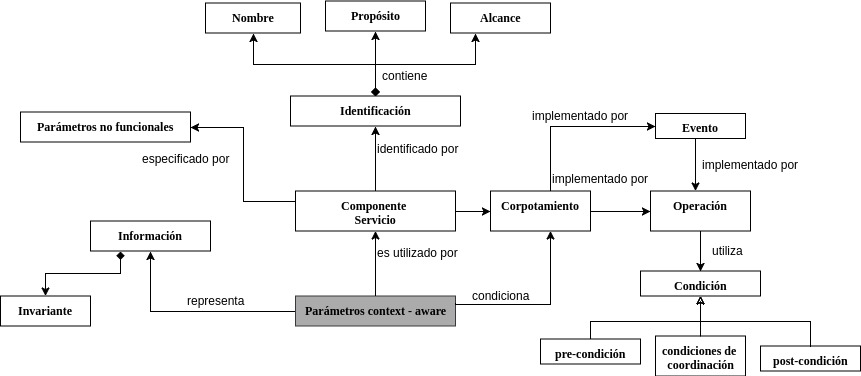
\includegraphics [width=6 in,totalheight=3 in]{Ch4/contrato_conceptual}
 % .: 0x0 pixel, 0dpi, 0.00x0.00 cm, bb=
\end{center}
% \caption{Características del ContratoDHD}
\label{fig:contratov2}
\end{figure}

A continuación, se describen para cada componentes sus principales características, roles y funciones que cumplen dentro 
del esquema conceptual general.


\begin{itemize}

\item \textit{Identificador}.

El \textit{Identificador} se utiliza para la identificación de una \textit{componente servicio} para un determinado contexto por un único nombre en un espacio de nombre.

\item \textit{Comportamiento.}

De acuerdo con los roles asignados en un determinado contexto, una
\textit{Componente Servicio} expone sus  \textit{comportamientos} a través de \textit{operaciones} publicadas. Las operaciones pueden ser definidas en dos tipos – operaciones que ejecutan cómputos o
transformaciones (tipo “update”) y operaciones que proveen algún tipo de información
sobre consultas (tipo “query”). Estas, se encuentran enteramente especificadas en base
a un contrato, con el uso de \textit{pre-condición}, \textit{post-condición} y \textit{condicionales} para lograr coordinación entre contratos. En las condiciones de coordinación se especifican cómo
requerir y proveer operaciones, así como también los eventos publicados y recibidos son coordinados en los momentos adecuados. Para lograr una comunicación precisa con una componente servicio, no sólo se tiene en cuenta qué operación fue provista o requerida y cómo el ejecutor ha lanzado el evento apropiado, sino también, cómo todas esas actividades están mutuamente relacionadas para ser aprovechadas por el objeto consumidor. Un evento del contexto que lanza una operación dada, puede ser parte de un conjunto de pre-condición, mientras que un evento emitido a través de una exitosa operación puede ser parte de una pos-condición.


Las operaciones provistas por la componente de servicio debenestar asociadas, a fin de determinar cuáles deben ser completadas antes de la activación de un servicio asociado. Este tipo de asociación es posible es posible de efectuarse en forma paralela o ser sincronizado por otro camino mecanismo. Por ejemplo, la figura \ref{fig:contratov2} representa el caso de una componente de servicio denominado \textit{Manejador\_Orden}, la operación \textit{ejecutar\_orden()} no puede ser invocada hasta que el servicio que la consume no esté correctamente autorizado por el componente de servicio \textit{Administrador\_Registros}. Otro ejemplo, la operación \textit{borrar\_registro()} no puede ser invocada si la operación \textit{ejecutar\_orden()} con el mismo parámetro \textit{orden\_id} no fue previamente completada.




\begin{figure}
\begin{center}
 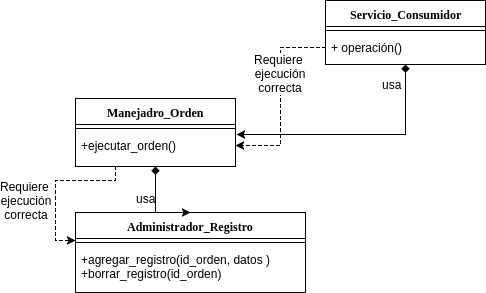
\includegraphics [width=3.5 in,totalheight=2 in]{Ch4/servicios_coordinados}
 % .: 0x0 pixel, 0dpi, 0.00x0.00 cm, bb=
\end{center}
\caption{Coordinación de servicios}
\label{fig:servicios_coordinados}
\end{figure}





\item \textit{Tipos de Información.}

Una componente de servicio debe manejar, usar, crear o tener
cierta información de recursos con el propósito de proveer servicios
adecuadamente.
Este elemento del contrato define el tipo de información relevante para las
componentes
asociadas al contrato, así como también restricciones y reglas sobre instancias
de esos
tipos. Esto representa un modelo de información lógica de una componente de
servicio.
Formalmente, esta información de tipos puede ser considerada como definiciones
de
tipos de los parámetros de las operaciones o tipos relacionados a ellos.


\item \textit{Configuración de Parámetros Context-Aware}

Una componente servicio depende del contexto de su actual entorno. La misma,
para utilizarse en diferentes contextos logrando la adaptación a eventuales
cambios debe tener definido un conjunto de parámetros de configuración. Ejemplos
de estos parámetros pueden ser: Contexto-del-Usuario (CU) - en un sentido
similar a lo definido en el capítulo
anterior, locación en tiempo y espacio de los servicios consumidos y
suministrados. Estos parámetros, pueden ser enviados dentro de las invocaciones
de las operaciones de los servicios o por medio de otros caminos, mediante
componentes de servicios que pueden adaptar su comportamiento ante el cambio de
contexto en una determinada situación.


La configuración de parámetros está directamente asociada a las relaciones de
las operaciones de los servicios para lograr una mejor adaptación a la medida de
las circunstancias brindada por la información relevada del contexto. El
concepto de la configuración de los parámetros context-aware, es un paso muy
importante hacia la concepción de servicios automatizados y auto adaptables
(tomando el sentido paradigmático de los teóricos de la Inteligencia
Artificial).


\item \textit{Parámetros no funcionales.} 

Una componente servicio puede definir un conjunto de los llamados parámetros no
funcionales que caracterizan a la “calidad” de sus prestaciones dentro de un
determinado contexto. Estos parámetros, son elementos para los consumidores de
los servicios que permiten optar por el uso de un determinado servicio, o buscar
otro con el mismo o similar contrato. Como ejemplo de parámetros no funcionales
podemos mencionar: Performance, Fiabilidad, Tolerancia a Fallos, Costos,
Prioridad y Seguridad.

\end{itemize}




\section{ContratosDHD: Contratos sensibles al contexto para el DHD}
\label{sec:estrategiasca}


Una vez más se abordará una definición teniendo en cuenta cuestiones
tecnológica inherentes a su implementación. La implementación
de los contratos para el DHD debe cumplir el dise\~no de la figura \ref{fig:
contratov2} a través de la metodología del agregado del framework JCA\footnote{JCAF is designed to support Context-Aware Computing and has
come out of our work with the design of context-aware applications in a hospital
environment.} (véase forma de agregado en la sección \ref{sec:subsistemas})
 



Para esta tesis se han explorado diferentes implementaciones de los
contratos de Meyer, preferentemente aquellas que se puedan ajustar mejor en
nuestro desarrollos y dise\~no. De esta manera, se tuvieron en cuenta avances
donde el uso de contrato para la representación de aserciones permitan
una buena integración para el DHD. Desafortunadamente, existen pocos lenguajes
que soportan técnicas de aserciones (ej. Eiffel \footnote{Eiffel fue ideado en
1985 por Bertrand Meyer. Es un lenguaje de programación orientado a objetos
centrado en la construcción de software robusto. Su sintaxis es parecida a la
del lenguaje de programación Pascal. Una característica que lo distingue del
resto de los lenguajes es que permite el diseño por contrato desde la base, con
precondiciones, postcondiciones, invariantes y variantes de bucle, invariantes
de clase y aserciones.}). Las forma de implementación y la tecnología (e.j.,
lengujes de programación, etc.) que se utiliza tienen una alta incidencia en
el dise\~no y arquitectura. En este sentido, se analizaron tres diferentes tipos
de estrategias de implementación.

\begin{itemize}
 \item \textbf{\textit{Built in}}: significa que el soporte de los contratos está
incluido en los el lenguaje de programación. Donde se tienen constructores de lenguajes para
la formulación de aserciones de diferentes formas. La corrección de la
sintaxis de la aserción es directamente chequeada por el compilador. Además,
el entorno de ejecución posibilita que se controle dicho chequeo en tiempo de
ejecución. Las mayores ventajas de estas implementaciones tienen que ver con la
homogenia integración de las aserciones dentro del lenguaje de
programación, i.e., los mensajes de error son consistentes, las herramientas de depuración
permiten un adecuado manejo e implementación de aserciones (ej., correctitud de número de línea y traza de ejecución).


\item \textbf{\textit{Preprocessing}}: Esta es la clase mas popular de soporte para las
aserciones en los lenguaje de programación. La idea general es la formulación
de aserciones separadas del programa o incluirlas como comentarios. Utiliza un
pre-proceso para entretejer aserciones entre el programa o transformar los
comentarios en porciones de código que la ejecuten. La principal ventaja de
este método es la separación entre el contrato y la lógica de programación.


\item \textbf{\textit{Metaprogramming}}: La metaprogramación refiere a 
"programación para los niveles de la interpretación de los
programas, o en otras palabras, para extender las interpretaciones de un
lenguaje de programación hacia una explicación específica"\cite{Temp1}.
Programas que tienen la posibilidad de razonar sobre si mismo tiene la
propiedad llamada reflectiva (en inglés ``reflective capacity``). Por ejemplo,
el lenguaje de programación Java tiene capacidades reflectivas y es
implementada a través de una API. La mayor ventaja de la metaprogramación es
que no es necesario el uso de preprocesamiento. No obstante, un entorno de
ejecución especializado debe ser usado para el chequeo de las aserciones.


\end{itemize}


\subsection{Sistema que proveen soportes para el desarrollo de software
basado en contratos} \label{sec:sistemasca}


Se analiza brevemente diferentes sistemas que proveen soporte para el
desarrollo de software basado en contratos a través del lenguaje de
programación Java. Estas propuestas fueron estudiadas en base a los prototipos
disponibles para evaluar el impacto en nuestra particular implementación,
i.e., no solamente una evaluación teórica. No fueron consideradas propuestas
que usan técnicas de álgebraicas o lógica de alto órden. De la misma manera
sistemas como JML \cite{Leavens99} no fueron considerados. 

A continuación se detalla para cada propuesta de sistema el nombre, el tipo de
resolución implementada (lenguajes de programación, extensiones de
lenguajes, preprocesamiento, metaprogramción), consideraciones generales,
características especiales y referencias.

\begin{itemize}
 \item Biscotti:

\begin{itemize}
\item \underline{Tipo de soporte}: Extensión del lenguaje Jaca; tiene
incorporado un
soporte para compilación.
\item \underline{Información}: Biscotti se concentra en la implementación de
especificaciones de comportamiento a través de interfases Java introduciendo
palabras claves adicionales. 

\item \underline{Características especiales}: No es necesario hacer cambios para
la
máquina virtual java, esto es posible debido a que Biscotti usa reflección y
facilita la creación de precondiciones, postcondiciones e invariantes visibles
en tiempo de ejecución.
\item \underline{References}: \cite{Cicalese99}
\end{itemize}

\item Java Assertion Facility (JAF):
\begin{itemize}
\item \underline{Tipo de soporte}: Implementado desde la versión 1.4 de Java.
\item \underline{Información}: Desde la versión 1.4 de Java se incorporó palabra
claves para aserciones para indicarles al compilador donde se encuentran
las aserciones y su interpretación a través de la máquina virtual. Java solo
soporta mecanismos de aserciones simples que permiten instrumentar condiciones
a través de métodos.
\item \underline{Características especiales}: El chequeo de las aserciones
pueden ser
fácilmente habilitadas y deshabilitada y los rastros de las aserciones pueden
ser completamente eliminados de los archivos de las clases. 
\item \underline{Referencias}:\cite{Sun02,Rogers01a,Rogers01b}.
\end{itemize}


\textbf{\item ContractJava:}
\begin{itemize}
\item \underline{Tipo de soporte}: ContractJava es el típico preprocesamiento en
el que se
genera código Java.
\item \underline{Información}: El preprocesamento soporta los usuales tipos de
precondiciones, postcondiciones y aserciones.
\item \underline{Características especiales}: Soporta comportamiento de
subtipo (Behavioral subtyping)\cite{subtyping}  
\item \underline{Referencias}: \cite{Findler01}
\end{itemize}

\textbf{\item iContract:}
\begin{itemize}
\item \underline{Tipo de soporte}: Preprocesamiento en el que se genera código
Java para
ser compilado por el compilador estándar Java.
\item \underline{Información}: Las aserciones son escritas como documentación de
métodos
y clases 
\item \underline{Características especiales}: iContract soporta operaciones
sobre
colecciones y provee herramienta adicionales para la documentación de
aserciones en Java Doc (iDoclet) y para facilitar el redise\~no de clases Java
(iDarvin)
\item \underline{Referencias}: \cite{Kramer98,Enseling01}
\end{itemize}

\textbf{\item Jass:}
\begin{itemize}
\item \underline{Tipo de soporte}: Preprocesador para la generación
de código Java  antes
de la copilación.
\item \underline{Información}: Los significados de las aserciones son
especificados por
medio de comentarios para métodos y clases. Un programa Jass es un programa
Java bien formado y puede ser transformado directamente para el compilador
estándar Java.
\item \underline{Características especiales}: Jass soporta
cuantificadores universales y
existenciales para conjuntos finitos. 
\item \underline{Referencias}: \cite{Bartezko01}
\end{itemize}


\textbf{\item Jcontract:}
\begin{itemize}
\item \underline{Tipo de soporte}: Preprocesador para la generación de código
java para
el compilador estándar Java.
\item \underline{Información}: Las aserciones se especifican como
comentarios para
métodos y clases.
\item \underline{Características especiales}: Jcontract soporta cuantificadores
existenciales y universales para tipos de los colecciones. Además, Jcontract
está estrechamente integrado con la herramienta Jtest\cite{Parasoft02a}. Jtest
la información de especificación contenida en el contrato, luego crea una
clase de test ejecutable que permite testear si se cumple la funcionalidad de
la clase especificada. Incluye herramienta de generación de javadoc para la
generación de documentación API donde contiene las especificaciones de las
aserciones. 
\item \underline{Referencias}:\cite{Parasoft02b}
\end{itemize}


\textbf{\item Handshake:}
\begin{itemize}
\item \underline{Tipo de soporte}: Provee aserciones a través de reflección
(Java
reflection). 
\item \underline{Información}: Los contratos son separados en archivos
diferentes. Las
clases son combinadas en tiempo de ejecución combinando dinámicamente los
archivos de los contratos y las clases Java.
\item \underline{Características especiales}: Debido a la propiedades dinámicas
los
contratos son incorporados a las clases a nivel de código de ejecución.
\item \underline{Referencias}:\cite{Duncan98}
\end{itemize}


\textbf{\item jContractor:}
\begin{itemize}
\item \underline{Tipo de soporte}: jContractor se basa puramente en librerías
base
utilizando metaniveles de información deducidas de los archivos de las clases
Java y usa la ejecución dinámica de las clases Java a través de la
interpretación de cambios reflectivos en tiempo de ejecución. 
\item \underline{Información}: La codificación del contrato (precondiciones,
postcondiciones e invanriantes) son incorporados a las clases por medios del
especificados con determinadas convenciones de nombres.
\item \underline{Características especiales}: Dentro de las postcondiciones de
un método
es posible controlar los resultados esperados con otros resultados específicos.
\item \underline{Referencias}:\cite{Parasoft02b} 
\end{itemize}
\end{itemize}
 
 
%\colorbox{yellow}{*** conectar esto ***}


Teniendo en cuenta las característica del modelos conceptual de contrato de la figura \ref{fig:contratov2} y las características de las infraestructuras utilizadas para su implementación, se comienza a determinar las primeras consideraciones a tener en cuenta en el diseño de contratos sensibles al contexto para el DHD.


\begin{defi} [ContratoDHD]
El ContratosDHD es una infraestructura para la aplicación del concepto de Diseño por Contrato (DbC) de Bertran Meyer (2002). El DbC es una técnica diseñada por Meyer y característica central de su lenguaje de programación Eiffel\cite{Meyer}. El DbC se utiliza con cualquier lenguaje de programación, para validar que el software cumpla con su especificación (contrato). El contrato establece condiciones de uso e implementación denominadas aseveraciones que componentes de software con un rol de "clientes" y otras de "proveedores" deben cumplir. En el DbC se utilizan tres tipos de aseveraciones: \underline{Precondición:} restricciones bajo las cuales una rutina funcionará correctamente.  \underline{Postcondición:} describe el efecto de la rutina. \underline{Invariante de clase:} restricciones que deben satisfacerse por cada objeto tras la ejecución de los métodos y constructores. 
Para la instrumentación de ContratosDHD se crearon dos tipos de componentes esenciales que permitan una correcta integración, a niveles de diseño e implementación, con una plataforma e-learning:

\begin{itemize} \label{CEC}

 \item Componente esencial tipo \#1: Componentes del contratos para la implementación de las
propiedades de sensibilidad al contexto. Los elementos que integran este
subsistema son:
 
      \begin{itemize}
       \item Arquitectura para la adaptación del contextos
       \item Funcionalidades 
      \end{itemize}
      
  \item Componente esencial tipo \#2: Componentes de conexión e implementación de un patrón de
dise\~no que permite la coordinación de contratos.
	    \begin{itemize}
	    \item Reglas de coordinación
		  
		  \begin{itemize}
		   \item Condicionales especiales
		   \item Condicionales comunes 
		  \end{itemize}
	    \item Componentes de conexión
	    \end{itemize}
\end{itemize}
\end{defi} 



\subsection{Componentes esenciales de los contratos sensibles al contexto}

En este apartado se exponen diferentes tipos de componentes para capturar datos de 
contexto. Estos datos serán representados en un modelos abstracto de información  utilizado para adaptar los servicios, de una aplicación, a los usuarios o artefactos de software que lo utilizan; en función de sus propios estados o estado del entorno. Para este propósito, se parte del modelo propuesto por A. Dey (2000) en su tesis doctoral \cite{Dey} que se propone una arquitectura conceptual para los sistemas sensibles  al contexto. A continuación, se enumeren las principales características de los elementos que definen esa arquitectura:


\begin{itemize}

\item \textbf {Servidor de contexto:}  Permite el acceso de múltiples
clientes a los datos de forma remota.  Libera a los clientes de
recursos que demandan operaciones intensivas.  Debe considerar el uso
de protocolos apropiados para la representación de las variantes de información de contexto, rendimiento de la red, calidad de lo parámetros de los servicios.


\item \textbf{Widgets}:  Encapsulamiento.  Intercambiable.
Controlado a través de un manejador de widget. En el caso que las
componentes estén acopladas incrementan la eficiencia al costo de perder robustez ante fallas de componentes.


\item \textbf{Networked services:}  Similar a la arquitectura
servidor de contexto. (modelo orientado a objeto).  tiene la eficiencia de la arquitectura \textbf{widget} debido a la complejidad de las componentes bases de red, pero provee robustez.


\item \textbf{Blackboard model:}  Procesos post-mensajes para
compartir medios, pizarrón (modelo basado en datos). Simplicidad en el agregado de nuevos recursos de contexto.  Fácil configuración.  Un servicio centralizado.  Carece de eficiencia en la comunicación (son
necesarios dos puntos de conexión por comunicación)

\end{itemize}

La componente \textit{Widget} cumple un importante papel en la propuesta de Dey. Un \textit{widget} es un componente de software que brinda una interfaz pública para algún tipo determinado de sensores (hardware) (Dey, A. K. y G. D. Abowd, 2000). Los \textit{widgets} encapsula detalles de datos censado a nivel de hardware. También, son componentes con alto grado de reusabilidad facilitando las tareas de diseño e implementación de aplicaciones en la s que se utiliza información de contexto capturadas por sensores. El encapsulamiento en los \textit{widgets} permite intercambiarlos entre aquellos que proveen el mismo tipo de datos (ejemplo:
intercambiar un \textit{widget} de radiofrecuencia por un \textit{widget} de una cámara filmadora donde ambos recolectan datos de locación de individuos).

Usualmente los \textit{widgets} son controlados por módulos de administrador de \textit{widget}. Una buena práctica para administrar \textit{widgets} es combinar sus funcionamientos de forma acoplada para incrementar su eficiencia, aunque esta decisión hace perder robustez ante fallas de componentes.

Ahora se presentan cinco categorías de componentes agregadas a las anteriores para el manejo del contexto.


\begin{itemize}
 \item {\textfb{Context Widgets:}} se encarga de la adquisición de información de contexto; 

\item {\textfb{Interpreters:}} cumplen la función de transformar y aumentar el
grado de abstracción de la información de contexto, deben combinar varias
piezas de contexto para producir información procesada de alto nivel;


\item {\textfb{Aggregator:}} es un componente que junta información de contexto
de una entidad para facilitar su acceso a las aplicaciones; 


\item {\textfb{Services:}} brindan servicios en un determinado ambiente
adaptando su funcionalidad al tipo de información de contexto adquirida; 

\item {\textfb{Discoveres:}} permite que las aplicaciones (y otras entidades)
optimicen su desempeño pudiendo determinar la característica del entorno
(tipo de restricciones y dominio de aplicación). Entre estos componentes
se pueden establecer un número limitado de relaciones.

\end{itemize}

Los widgets son consultados y/o notificados ante eventuales cambios en los
de información del estado del cliente. Los clientes pueden ser \textit{aplicaciones}, \textit{aggregators} u
otros \textit{widgets}. A su vez, \textit{aggregators} actúa como un puente entre \textit{widgets} y aplicaciones. Un \textit{interpreters} puede ser solicitado en un determinado estado por un \textit{widget}, \textit{aggregator} o \textit{aplicaciones}. Los \textit{services} son lanzados por las aplicaciones (también otros componentes pueden hacer uso de los servicios). \textit{Discoveres} se comunica con todos los componentes, se adquiere desde los \textit{widget}, \textit{interpreters} y \textit{aggregators}, y provee información a las aplicaciones por medio de notificaciones y consultas.

La figura \ref{fig:toolkit} expone una posible configuración con dos
dispositivos de censado, dos \textit{widgets}, un \textit{aggregator}, dos
\textit{interpreters}, un \textit{servicio}, un \textit{discoverer} y dos
\textit{aplicaciones}.



\begin{figure}
\begin{center}
 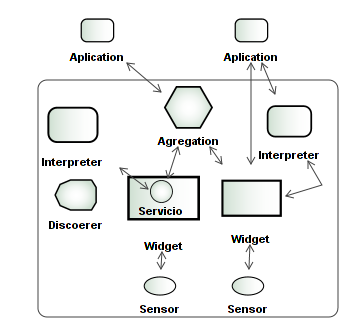
\includegraphics [width=5 in,totalheight=2 in]{Ch4/ContextToolsKit.png}
\caption{Elementos para la toma de contexto en los ContratosDHD}
\label{fig:toolkit}
 % .: 0x0 pixel, 0dpi, 0.00x0.00 cm, bb=
\end{center}
\end{figure}


En el instante en que algún componente contexto se encuentre disponible,
registra sus capacidades en un \textit{discoverer}. Esto permite que los
\textit{aggregators}
encuentren \textit{widgets} e \textit{interpreters} y, a las aplicaciones,
encontrar \textit{aggregators},
\textit{widget} e \textit{interpreters}. Un sensor provee datos para un
\textit{context widget}, el cual se encarga de almacenar el contexto. Puede
llamar a un \textit{interpreter} para obtener
un mayor nivel de abstracción de los datos y luego pone el contexto a
disposición (para que pueda ser accedido) por otros componentes y aplicaciones.

Un \textit{aggregator} recolecta información de contexto de las entidades,
representadas por los \textit{widgets}. Finalmente, las aplicaciones pueden
consultar o
suscribirse a los \textit{agreegators} (o directamente con los \textit{widgets},
si se quiere) y
llamar a \textit{interpreters} (si el deseado nivel de abstracción no se
encuentra
disponible desde los \textit{widgets} y \textit{aggregators}).

Estos componentes se ejecutan independientemente de las aplicaciones, asegurando
una continua adquisición de información de contexto y el uso de múltiples
aplicaciones. Además, todos los componentes y aplicaciones se comunican entre
ellos automáticamente usando protocolos y lenguajes conocidos.

Esto da lugar a que los programadores que implementan un particular componente o
aplicación puedan comunicarse con otro componente sin tener conocimiento de los
mecanismos usados para lograr la interacción.


\subsection{Una implementaci´o del subsistema para CEC\#1}

La implementaci´on del subsistema de las componentes esenciales para el
agregado de propiedades de sensibilidad al contexto (CEC\#1) tienen dos
significancia para esta tesis. En primer lugar, es brindar un ejemplo concreto
de intregraci´on utilizando parte del recorrido te´orico y documental
de tipos de sistemas (secciones \ref{sec:sistemasca})  y estrategias (secciones
\ref{sec:estrategiasca}). En segundo lugar, presentar nuevos conceptos y
definiciones que permitan generalizar este tipo de propuestas de comunicaci´on
entre sistemas. 

Para este caso se utiliza como subsistema para CEC\#1 el framework JCAF 
(\textit{Java Context-Awareness Framework}). A través de JCAF se implementan
la ejecución de servicios (servicios de herramientas colaborativas) por medio de
la infraestructura orientada a servicios basada en la idea de la divisi´on de la
adquisición de contexto, su manejo y  distribuci´on o conexión con los
\hyperref[contratosDHD]{ContratosDHD}. Además JCAF provee un modelo de
programaci´on para Java extensible, gen´erico y expresivo orientado al
desarrollo e implementación de aplicaciones sensibles al contexto y modelado
de contexto. En la  publicaci´on \cite{JCAF} se brindan m´as detalles sobre
c´omo JCAF difiere de otros soporte middleware para aplicaciones sensibles al
contexto. 


Para describir m´as apropiadamente la participaci´on que JCAF tiene para 
nuestra propuesta de implememtaci´on es necesario determinar cu´ales de los
aspectos orientados a servicios ser´an recogidos. De esta manera se brinda una
defici´on sobre el contexto en el que se tienen en cuenta los servicios.


\begin{defi}[ServiciosDHD:] \label{serviciosDHD}
Se denomina servicioDHD a cualquier implementaci´on sobre las funcionalidades
de una herramienta, de un espacio colaborativo, (1) que tenga interfases de
comunicaci´on con la componente par´ametros Context-Aware (figura
\ref{fig:contratosv2}) y  (2) tiene su implementaci´on contiene elementos que
representan entidades participantes e informaci´on de contexto \cite{Dey}. En
otras palabras, la implementaci´on de un servicioDHD est´a compuesta por
m´odulos para la representaci´on y uso contexto y que los mecanismos de
ejecuci´on est´en mediado por los \hyperref[contratosdhd]{ContratosDHD} 

\end{defi}


\subsubsection{Infraestructura para serviciosDHD}


A partir de la infraestructura que brinda JCAF para combinar modelos e
implementaciones de servicios con informaci´on de contexto, se despliega una
serie de articulaciones que permita una daptaci´on para el uso de contratos. De
esta manera quedar´a conformada una nueva infraestructura para los
\hyperref[serviciosDHD]{serviciosDHD}.  

\colorbox{green}{La parte mas importante}



\begin{figure}
\begin{center}
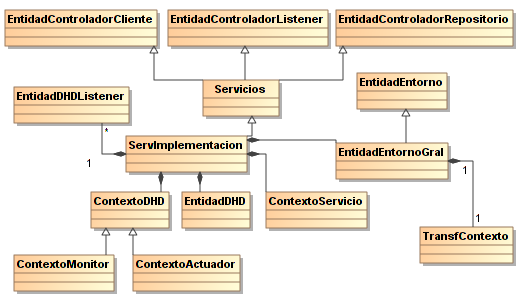
\includegraphics[width=5 in,totalheight=3.2 in]{Ch4/jcaf.png}
% .: 0x0 pixel, 0dpi, 0.00x0.00 cm, bb=
\caption{Arquitectura de ejecución de serviciosDHD}
\label{hiperplanos}
\end{center}
\end{figure}


\subsection{Coordinación de los contratos sensibles al contexto}


Elementos de la componente contrato La componente contrato es la información que se tiene de una componente. El contrato puede ser configurado por medio de diferentes mecanismos, desde el lenguaje cotidiano hasta un lenguaje de especificación formal y un lenguaje basado en XML2 para los casos en que sean necesarias especificaciones que puedan ser procesadas por máquinas.

El tipo de tecnología y forma de implementación de los contratos es transparente para los objetos que consumen los servicios en donde se encuentran involucrados. La configuración de un elemento contrato que forma parte de las componentes de un servicio representa la información necesaria del mismo para ser utilizado por el invocador, sin necesidad de que el objeto invocador tenga
detalles de la ejecución.

El contrato representa una enriquecida y efectiva interfaz de construcción que contiene toda la información sobre las componentes de los servicios y deberá tener información sobre algún tipo de información de contexto para su utilización.

En este caso, el concepto de interfaz tiene mayor significación que un simple acceso a un contrato de reglas entre el objeto proveedor del servicio y el objeto consumidor.

En la figura 2 podemos observar los elementos conceptuales básicos de esta
componente a través de una serie de elementos en relación con el contrato.
Este metamodelo tiene las características conceptuales y operativas que se
fundamentan en “Obra abierta”.

Para una mejor comprensión de las componentes del modelo explicitaremos
a continuación su caracterización y funciones particulares.

\textbf{Identificador}: una componente servicio es identificada para un
determinado
contexto por un único nombre en el espacio de identificación.

\textbf{Comportamiento}: de acuerdo con los roles asignados en un determinado
contexto, una componente servicio expone comportamientos correspondientes a
provisión y pedido de operaciones, y/o publicaciones y recepción desde/hacia
cada contexto. Las operaciones pueden ser definidas de dos tipos: operaciones
que ejecutan cómputo o transformaciones (tipo update) y operaciones que proveen
algún tipo de información sobre consultas (tipo query). Éstas se encuentran
enteramente especificadas en base a un contrato, con el uso de precondición,
poscondición y condicionales para lograr la coordinación entre contratos. En las
condiciones de coordinación se especifican cómo requerir y proveer operaciones,
así como también los eventos publicados y recibidos son coordinados en los
momentos adecuados. Para lograr una comunicación precisa con una componente
servicio, no sólo se tiene en cuenta qué operación fue provista o requerida
y cómo el ejecutor ha lanzado el evento apropiado, sino también cómo todas
esas actividades están mutuamente relacionadas para ser aprovechadas por el
objeto consumidor. Un evento del contexto que lanza una operación dada
puede ser parte de un conjunto de precondición, mientras que un evento emitido
a través de una exitosa operación puede ser parte de una poscondición.


Las operaciones provistas y requeridas por la componente de servicio
deben estar asociadas, a fin de determinar las operaciones que deben ser completadas
antes de la activación de un servicio (qué es posible ejecutar en paralelo
o ser sincronizado por otro camino). Por ejemplo, en el caso de una
componente de servicio ManejadorOrden, la operación HacerOrden no puede
ser invocada hasta que el servicio que la consume no esté correctamente autorizado
por el componente de servicio AdministradorRegistros, o la operación
DeleteOrder no puede ser invocada si la operación HacerOrden con el mismo
parámetro OrdenID no fue previamente completada.
Tipos de información: una componente de servicio debe manejar, usar, crear o
tener cierta información de recursos con el propósito de proveer servicios adecuadamente.
Este elemento del contrato define el tipo de información relevante
para las componentes asociadas al contrato, así como también
restricciones y reglas sobre instancias de esos tipos. Esto representa un modelo
de información lógica de una componente de servicio. Formalmente, esta
información de tipos puede ser considerada como definiciones de tipos de los
parámetros de las operaciones o tipos relacionados a ellos.
Configuración de parámetros context-aware: una componente servicio depende
del contexto de su actual entorno. La misma, para utilizarse en diferentes contextos
logrando la adaptación a eventuales cambios, debe tener definido un
conjunto de parámetros de configuración. Ejemplos de estos parámetros pueden
ser: Contexto del Usuario (CU), en un sentido similar a lo definido en el
capítulo anterior, locación en tiempo y espacio de los servicios consumidos y
suministrados. Estos parámetros pueden ser enviados dentro de las invocaciones
de las operaciones de los servicios o por medio de otros caminos, mediante
componentes de servicios que pueden adaptar su comportamiento ante el
cambio de contexto en una determinada situación.
La configuración de parámetros está directamente asociada a las relaciones
de las operaciones de los servicios para lograr una mejor adaptación a la
medida de las circunstancias brindada por la información relevada del contexto.
El concepto de la configuración de los parámetros context-aware es un
paso muy importante hacia la concepción de servicios automatizados y autoadaptables
(tomando el sentido paradigmático de los teóricos de la inteligencia
artificial).

\textbf{Parámetros no funcionales:} una componente servicio puede definir un
conjunto de los llamados parámetros no funcionales que caracterizan la “calidad”
de sus prestaciones dentro de un determinado contexto. Estos parámetros
son elementos para los consumidores de los servicios que permiten optar por el
uso de un determinado servicio, o buscar otro con el mismo o similar contrato.
Como ejemplo de parámetros no funcionales podemos mencionar: performance,
fiabilidad, tolerancia a fallos, costos, prioridad y seguridad.


\subsubsection {Coordinación}

En términos generales, la coordinación de contratos es una conexión establecida
entre un grupo de objetos (en nuestras consideraciones los participantes
serían un objeto cliente y un determinado servicio), donde reglas, normas y
restricciones (RNR) son superpuestas entre los actores participantes, estableciendo
con un determinado grado de control las formas de interrelación (o
interacción).

El tipo de interacciones establecidas entre las partes es más satisfactoria
que las que se pueden lograr con UML o lenguajes similares (orientados a objetos)
debido a que éstas contienen un mecanismo de superposición donde se
toman como argumento los contextos. Cuando un objeto cliente efectúa una
llamada a un objeto suministro, el contrato “intercepta” la llamada y establece
una nueva relación teniendo en cuenta el contexto del objeto cliente, el
del objeto servidor e información relevante (respecto de la relación) adquirida
y representada como contexto del entorno. Como condición necesaria, la
implementación de los contratos no debe alterar el diseño y funcionalidad en
la implementación de los objetos.


\section{Condicionales especiales para las reglas de los contratos}

En las implementaciones de campo de cursos de nivel superior realizadas por
el equipo de “Obra abierta”, uno de los recursos primarios que los educadores
utilizaban era el registro de actividades de la plataforma. Podemos ahora considerar
una información de contexto, a un valor cuantitativo que resignifique
una característica del comportamiento de un usuario, tal como lo expusimos
en el \ref{}.

Consultar los registros de actividades es una práctica muy usual para obtener
información sobre el “grado” de interactividad que los usuarios tienen en el
marco del dispositivo hipermedial. En los casos más básicos, existe una estructura
de “planilla” (filas y columnas) en las que se detallan los registros con los
siguientes campos: fecha, hora, usuario, tareas realizadas. Las tareas pueden estar
significadas con valores literales como: “visitas al foro”, “visualización de perfiles
de usuarios”, “obtención de recursos”, “modificación datos de la wiki”, etcétera.

El “grado” de interactividad como información de contexto fue observado
específicamente durante la experiencia de taller expuesta en el capítulo IV
bajo el título “Un diseño de taller físico-virtual-interactivo-comunicacional”.
Retomando esta temática y atendiendo a la posibilidad de usar la información
de interactividad como parámetro context-aware de los contratos según lo referido
en “Elementos de la componente contrato”, de este mismo capítulo,
podremos establecer un lazo de retroalimentación entre las prácticas efectuadas
en la plataforma Moodle, establecidas en el registro de actividades y las
acciones que devengan de los contratos.
En esta sección utilizaremos un modelo particular de métrica y una propuesta
de integración de dicho modelo al framework del dispositivo hipermedial
dinámico a través de los contratos context-aware.



\subsection{MCondicionales}

Para atender a los requerimientos anteriores, en primer lugar contamos con la
aplicación Moodle con el agregado de la componente adicional contrato. El
contrato fue incorporado a la herramienta foro de Moodle, mediante un prototipo
experimental siguiendo el modelo arquitectónico desarrollado en el
capítulo \ref{}.

Cabe destacar que, si bien lo fundamentado sobre el agregado de la componente
contrato a la arquitectura original de la plataforma está referido al
proyecto Sakai, la misma es similar a la que proponemos para Moodle. En
segundo lugar, diseñamos un mecanismo de métrica que fue usado como parte
esencial de las reglas de los contratos, tomando como referencia un modelo de
estandarización bien definido. Particularmente, la métrica formará parte del
condicional de las reglas del contrato. A estos tipos de condicionales los denominaremos:
“Mcondicional”. Conceptualmente no existe diferencia entre un Mcondicional y una
condición común, los valores de verdad de ambos pueden depender de la invocación
de métodos o funciones programadas para el sistema y colaborarán en la
articulación de la ejecución de acciones (servicios y procesos computacionales).

Al incorporar las métricas en el modelo original de contratos contextaware,
proponemos que el sistema sea más adaptable a nuevos cambios del contexto de
usuario (por ejemplo, en concordancia con el tipo de interacción de la
herramienta foro). Esto implica que las reglas que se pueden establecer
para el contrato se formulan en el marco de la complejidad de los procesos
didácticos (o investigativos y/o productivos), entendiendo que los mismos
siempre exceden la posibilidad de ser absolutamente reglados. Por lo tanto, las
mencionadas reglas estarán singularizadas en función de la dinámica de dichos
procesos, debiendo ser explícitas y de clara implementación y por sobre todo,
adaptables para los contextos específicos de los usuarios (en este caso, estudiantes
a nivel de grado).

El primer paso es lograr la explicitación de las reglas del contrato y que
los condicionales representen criterios de decisiones sobre aspectos relevantes
del proceso didáctico (investigativo o productivo). Por ejemplo, un estudiante
puede adquirir un servicio determinado de una herramienta, previo a la
evaluación de una condición representada como condicional de una regla.
En general, a estas reglas debemos diseñarlas con el cuidado de no incorporar
redundancias, ambigüedades o incoherencias, tanto entre las propias
reglas de un contrato como con otras reglas implícitas que se desprenden de
los servicios. De esta manera, definimos las reglas del contrato como un conjunto
de condiciones, acciones y prioridades.

La condición es un expresión Boolean sobre relaciones (mayor, menor,
igual, distinto, etc.) entre parámetros y valores concretos.
Las acciones conforman un conjunto de asignaciones de valor a otros parámetros
también definidos por el tipo de regla. Algunos de los parámetros de
las acciones deben ser “métodos de cálculo” que permitan cambios en el comportamiento
de los servicios en los cuales estas reglas son aplicadas.
La prioridad permite simplificar la cantidad de reglas que se deben escribir:
en lugar de la escritura de una regla para cada combinación de posibilidades
de los valores de los parámetros, se asegura que dos reglas no puedan ser
ejecutadas simultáneamente. El usuario podría escribir una prioridad baja para
todas las reglas y luego, con prioridades altas, ir identificando las excepciones
para el caso configurado inicialmente.

En síntesis, las reglas son ejecutadas mediante un orden de prioridades. En
consecuencia, en cada tipo de regla, cada una tiene sólo una prioridad.
Para ejemplificar este concepto, consideremos una regla donde, dependiendo
del tipo y cantidad de interacciones de un sujeto en formación (por
ejemplo, Juan Pérez), el servicio de la herramienta foro, es readaptado. Cabe
aclarar que en este caso, la acción del contrato establece el valor de calificación
de la intervención del usuario Juan Pérez en los temas tratados en los
foros. Entonces, el valor de verdad (Boolean) del condicional (donde parte de
la expresión está representada por el predicado: \textit{getForumTheme mayor a:
Minimus\_Forum\_Theme} ) depende de la ejecución de una métrica, debido a
que el método getForumTheme lanza el proceso de ejecución representado por
el subsistema de métrica asociado a las reglas del contrato.
Tal como lo mencionamos, estos tipos de condicionales fueron denominados
Mcondicionales y se pueden visualizar en el ejemplo. En la próxima sección
brindaremos los detalles técnicos y conceptuales sobre cómo se produce

la integración del subsistema de métrica como si fuera un sistema externo
conectado por la componente contrato.


\begin{verbatim}
If (getStudent = 'Juan') and (getForum_theme > Minimus_Forum_Theme)
Then
setPermissionQualifyForum ('Juan', Max_Forum_Qualify)
\end{verbatim} 
\caption {Ejemplo: Reglas de contratos con Mcondicionales}


\subsubsection {Modelo de integración}

Para implementar la invocación de métricas mediante métodos correctos, propusimos
desde la perspectiva del rediseño e implementación computacional,
un modelo de integración de muy bajo costo, sin cambios sustanciales ni en la
arquitectura original ni en el código de la implementación.

El modelo conceptual de métrica pertenece al Modelo INCAMI (Information Need, Concept model, Attribute, Metric and Indicador: Información relevante, Modelo Conceptual, Atributos, Métricas e Indicadores) (Olsina, L., G. Lafuente y G. Rossi, 2000). INCAMI es un framework organizacional, orientado a la medición y evaluación que permite economizar consistentemente, no sólo metadata de métricas e indicadores, sino también valores mensurables en contextos físicos.


Por medio de un diagrama UML, se representa un modelo global de integración, teniendo en cuenta experiencias vinculadas al agregado de nuevas componentes en determinadas implementaciones resueltas para sistemas elearning similares Sakai. La integración contempla, por un lado, el modelo de coordinación de contrato (enmarcado en el área de contrato, y por el otro, el modelo de métrica propuesto por Olsina (Olsina, L. y G. Rossi, 2002). En la figura 3 podemos observar lo correspondiente a cada una de las áreas mencionadas. La figura 3 también nos muestra que la principal componente para lograr la integración está representada por la incorporación de una relación de agregación entre la componente contrato, representada por una clase en el modelo UML y la entidad método. Los condicionales de las reglas de los contratos son
invocados (mediante un método explícito relacionado con la noción de los
Mcondicionales, por ejemplo, getForumTheme) por medio de un mecanismo
de callback que permite la correcta invocación de la métrica. El modelo de
métrica proporciona una implementación y diseño de adecuadas métricas para

suplir los requerimientos de interacción referidos al registro de actividades. Si
tenemos en cuenta el proceso de definición de métricas, debemos crear métricas
por cada atributo. Definido en una estructura denominada árbol de requerimiento
(tema que desarrollaremos más adelante), cada atributo puede ser
cuantificado por más de una métrica.
Cabe aclarar que este proceso de confección de métricas, podemos considerarlo
como una metodología propia con fines específicos de esta área disciplinar
de la ciencia.
Las métricas contienen la definición de métodos y escalas para un determinado
tipo de medición y/o cálculo. Dada una métrica m representa una relación
(mapeo) m: A→ X, donde A es un atributo empírico de una entidad (el
mundo empírico), X es la variable en la cual se asignarán (o pueden ser asignados)
valores categóricos y numéricos (el mundo formal), y la flecha denota
la relación de mapeo (mapping). Para lograr el mapping, es necesaria una
correcta y precisa definición de actividades de medición por medio de una
especificación explícita de los métodos de las métricas y las escalas tal como
podemos ver en la figura \ref{}.

Para las métricas directas, podemos aplicar métodos de mediciones objetivos
y subjetivos, en cambio las métricas indirectas sólo pueden ser calculadas
mediante funciones, con la intervención de fórmulas lógicas/matemáticas.


\subsection{DMCondicionales}

Como ya observamos, existen diferentes alternativas para lograr la integración
de modelos por medio de un contrato. En este sentido, planteamos en
la sección anterior un modelo de integración donde, por medio de los condicionales
de las reglas, se invocaban métodos de un modelo externo.
Ahora proponemos una nueva integración de un modelo externo que permitirá,
aplicando la minería de datos, enriquecer aún más la semántica de
los contratos.

Estado actual de la aplicación de la minería de datos a los sistemas
de enseñanza mediados por la web
En este apartado nos introduciremos en aspectos relevantes del estado del arte
en la investigación sobre la aplicación específica de técnicas de minería de
datos a los sistemas de enseñanza mediados por la web o sistemas e-learning.
Tanto la minería de datos como dichos sistemas son áreas que muestran
importantes desarrollos, y la vinculación de las mismas está suscitando un creciente
interés por parte de investigadores y empresas.

Entre los diferentes métodos y técnicas existentes de minería de datos,
nos hemos centrado principalmente en la minería de utilización web, concretamente
en la clasificación y agrupamiento, descubrimiento de reglas de asociación
y secuencias de patrones, ya que son técnicas motivadas por los
mismos requerimientos planteados en este capítulo y fundamentados en la
perspectiva de “Obra abierta”.

Asumimos que en los sistemas e-learning el principal objetivo de la utilización
de técnicas de data mining (minería de datos) es proveer mecanismos
que permitan guiar a los estudiantes durante su aprendizaje, con el propósito
de incrementar las facilidades y servicios para la obtención de información y
conocimiento calificado.

Las técnicas más utilizadas en la minería de datos aplicada a los sistemas
de e-learning son: clasificación y agrupamiento, descubrimiento de reglas de
asociación y análisis de secuencias. A continuación, vamos a exponer brevemente
los principales trabajos de investigación agrupados dentro de estos tres
tipos de técnicas, aunque algunos investigadores utilicen no una, sino varias.
Clasificación y agrupamiento.

Las técnicas de clasificación y agrupamiento o clustering (Arabie, P., J. Hubert
y G. de Soete, 1996) consisten en la habilidad intelectual para ordenar o dividir
fenómenos complejos (descriptos por conjuntos de objetos con datos altamente
dimensionales) en pequeños y comprensibles unidades o clases que
permiten un mejor control o comprensión de la información.

Su aplicación a sistemas e-learning permite agrupar a los usuarios por su
comportamiento de navegación, agrupar las páginas por su contenido, tipo o
acceso y agrupar similares comportamientos de navegación. A continuación
describiremos algunos trabajos de aplicación de minería de datos en educación.

La técnicas de agrupamiento son utilizadas por Gord McCalla y Tiffany
Tang (Tang, T. y G. McCalla, 2004) para formar clusters o grupos de usuarios
basándose en su comportamiento de navegación, aplicando un algoritmo de
clustering basado en largas secuencias generalizadas. También proponen incluir
un sistema recomendador inteligente dentro de un sistema de aprendizaje
basado en web evolutivo capaz de adaptarse no sólo a sus usuarios, sino también
a la web abierta. El sistema puede encontrar contenidos relevantes en la
web pudiendo personalizar y adaptar sus contenidos, basándose en observaciones
del sistema y por las propias valoraciones acumuladas dadas por los
miembros en formación.

Otro trabajo que también emplea agrupamiento es el realizado por Elena
Gaudioso y Luis Talavera (Romero, C., 2003) en el que analizan los datos
obtenidos de cursos basados en sistemas e-learning y utilizan técnicas de
clustering similares al modelo probabilístico de Naive Bayes para descubrir
patrones que reflejan comportamientos de los usuarios. El objetivo es utilizar
la minería de datos para dar soporte a la tutoría en comunidades de aprendizaje
virtual.

La utilización conjunta de clustering con otras técnicas como secuenciación es
realizada por Julia Miguillón y Enric Mor (Mor, E. y J. Minguillón, 2004) para
analizar el comportamiento de navegación de los usuarios para la personalización
del e-learning. Utilizan clustering de estudiantes para intentar extender las
capacidades de secuenciación de algunos sistemas estándares de manejo
de aprendizaje como SCORM para incluir el concepto de itinerario recomendado.

Los autores Erkki Sutinen y otros (Sutinen, E., W. Hämäläinen, J. Suhonen y H.
Toivonen, 2004) proponen un modelo híbrido que combina técnicas de minería de
datos y de aprendizaje de máquinas para la construcción de una red bayesiana
(http://es.wikipedia.org/wiki/Red\_bayesiana) que describe el proceso
de aprendizaje de los estudiantes. Su objetivo es clasificar a los estudiantes
para poder ofrecerles diferentes guías, dependiendo de sus habilidades y otras
características. Esta tarea se realiza con la categorización y clustering de los
estudiantes en base a sus habilidades o conocimiento. Finalmente, el
trabajo realizado por Jing Luan (Romero, C., 2003) utiliza técnicas de minería
de datos en educación superior y propone la utilización conjunta de predicción
y clustering dentro de una herramienta de soporte de decisiones permitiendo a 
la universidad prever las necesidades de los estudiantes.

Antecedentes de técnicas de minería de datos Las principales aplicaciones de las
técnicas de minería de datos en educación son sistemas de personalización
(Srivastava, J., B. Mobasher y R. Cooley, 2000), sistemas recomendadores (Li, J.
y O. Zaiane 2004), sistemas de modificación (Perkowitz, M. y O. Etzioni, 1998),
sistemas de detección de irregularidades (Barnett, V. y T. Lewis, 1994),
etcétera, debido a sus capacidades para el descubrimiento de patrones
de navegación regulares e irregulares, clasificaciones de alumnos y de los
contenidos, construcción adaptativa de planes de enseñanza, descubrimiento de
relaciones entre actividades, diagnóstico de los estudiantes, etcétera.

Reglas de los contratos y los DMcondicional El uso de reglas es una de las
formas más usuales de representación del conocimiento debido, entre otras
razones, a su sencillez, capacidad de expresión y escalabilidad. Dependiendo de
la naturaleza del conocimiento que almacenan, se ha establecido una tipología
informal para este tipo de estructuras. Así, se habla de reglas de decisión,
asociación, clasificación, predicción, causalidad, optimización, etc. En el
ámbito de la extracción de conocimiento en bases de datos, las más estudiadas
han sido las reglas de asociación, de clasificación y de predicción.


Las reglas de clasificación tienen como objetivo almacenar
conocimiento encaminado a la construcción de una clasificador preciso. En su
antecedente contienen una serie de requisitos (en forma de condiciones) que debe
cumplir un objeto determinado para que pueda considerarse perteneciente a la
clase identificada con el consecuente de la regla. Desde el punto de
vista sintáctico, la principal diferencia con las reglas de asociación es que 
presentan una sola condición en el consecuente, que además pertenece a un
identificador de clase.


La estructura de una regla puede ser caracterizada (en términos
generales) mediante un conjunto de condicionales lógicos en los que se fija un
criterio de ejecución de la acción. En este ejemplo, se verifica en el usuario
“alumno”, si su nivel de interacción en el foro pertenece a la clase de alto, y
si la calidad de sus intervenciones se encuentran en un rango aceptable. Este
tipo de información es obtenida del registro de actividades de la plataforma.


Supongamos, ahora, que los valores de estos dos últimos condicionales se
obtienen a partir de la ejecución de un algoritmo tipo TDIDT (Top-Down Induction
of Decision Trees), entonces, debe ser invocado el algoritmo por medio de un
método (en este caso, getCalidadIntervencion) a través de una regla explícita
en el contrato, de la siguiente manera:

\begin{verbatim}

if (usuario = ‘alumno’) and getCalidad_Intervencion = ‘aceptable’)
and this.getCantidad_Interaccion=‘alto’)
then herramienta.accion ()

\end{verbatim} 

Interesa destacar la estructura de la regla Si-entonces (If-Then) y los condicionales
de los cuales se desprende la ejecución de un algoritmo de data mining.
En este ejemplo, este tipo de condicional se muestra subrayado; y lo denominaremos
\textit{MDcondicional} (en lo conceptual, tenemos gran similitud con los
\textit{Mcondicionales} de la sección “Métricas de interacción para ‘Obra
abierta’”). De esta manera, por medio del \textit{MDcondicional}, se capturan
los resultados de la inferencia del árbol de decisión que se ilustra con la
figura \ref{}.

\begin{figure}
\begin{center}
 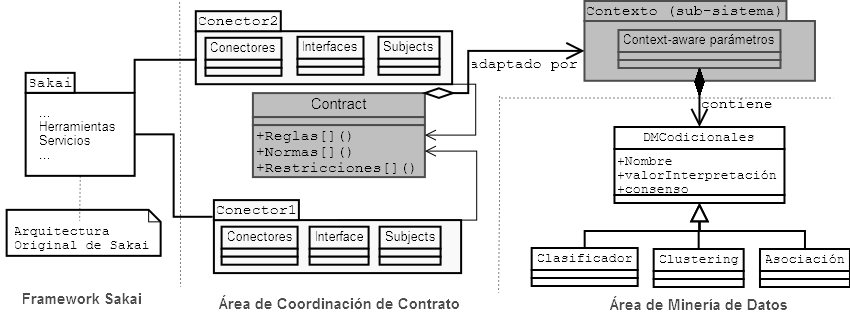
\includegraphics[width=6 in,totalheight=2 in]{Ch4/f3.png}
 % .: 0x0 pixel, 0dpi, nanxnan cm, bb=
\end{center}
\caption{Modelo de integración de los MDCondicionales}
\end{figure}


En las secciones posteriores nos introduciremos en las propuestas y justificaciones
para la incorporación de las técnicas de minería de datos a través
de los \textit{MDcondicional}.

Algoritmos de construcción de los \textit{MDcondicionales} Una de las formas más
simples
de representar conocimiento es mediante árboles de decisión. Dicha estructura de
representación del conocimiento está formada por una serie de nodos, donde: cada
nodo interno es etiquetado con el nombre de uno de los atributos predictores;
las ramas que salen de un nodo interno son etiquetadas con los valores del
atributo de ese nodo; cada nodo terminal, o nodo hoja, es etiquetado con el
valor del atributo objetivo.

Un ejemplo de árbol de decisión se muestra en la figura 4, donde el
atributo objetivo es el atributo nivel de aceptación y los atributos predictores
son lo atributos: interacción, respuestas, evaluación, consultas. Una
característica muy interesante de los árboles de decisión es que, a
partir de ellos, es muy fácil derivar un conjunto de reglas de producción del
tipo Si-entonces (If-Then) completamente equivalente al árbol original. El
algoritmo que nos permite realizar este cambio de modelo de representación
es casi trivial y convierte cada camino que va desde el nodo raíz hasta una
hoja, en una regla de la siguiente forma: los nodos internos y sus correspondientes
ramas de salida son convertidos en las condiciones del antecedente de la regla; los nodos hojas se convierten en el consecuente de la regla. Al convertir el árbol de decisión en una colección de reglas se obtiene una regla por hoja del árbol. Dichas reglas serán, por tanto, mutuamente excluyentes.

El algoritmo de construcción de árboles de decisión más popular es el algoritmo ID3 (Quinlan, J. R., 1987). Este algoritmo está basado en la división sucesiva y construye el árbol de decisión desde la raíz hacia las hojas, incrementando en cada paso la complejidad del árbol.

Inicializar T con el conjunto de todas las instancias Si (todas las instancias en el conjunto T satisfacen el criterio de parada) Entonces Crear un nodo hoja etiquetado con el nombre de la clase y  parar.

Sino Seleccionar un atributo para utilizar como atributo de particionado.
Crear un nodo etiquetado con el nombre del atributo y crear una rama por cada valor del atributo.
Particionar T en subconjuntos tales que contengan las instancias que cumplan los valores del atributo.

Aplicar este algoritmo recursivamente para cada subconjunto.
Fin Si Recorrer el árbol y formar las reglas.


\subsubsection{Modelo de integración}

Para lograr la incorporación de la componente data mining, volvemos a proponer
una nueva integración a muy bajo costo, desde el punto de vista del
rediseño e implementación con el propósito de facilitar la misma y el impacto
en la modificación de los módulos estándares de la aplicación e-learning. En
particular, Sakai, a diferencia de Moodle, provee una arquitectura en la que es
posible trabajar bajo el paradigma orientado a objetos (POO), con toda la
potencia y versatilidad de la tecnología Java, motivo por el cual se logra una
mejor adaptación del modelo de la componente conceptual data mining
mediante un correcto diseño orientado a objeto (DOO) (Grady, B., 1982).
En la figura 5, representamos el contrato con un diagrama de clase. Las
reglas, normas y restricciones (RNR) están representadas con tres métodos
independientes en el diagrama de la clase contrato.
Teniendo en cuenta la analogía planteada entre las reglas del contrato y la
estructura de los árboles que determina el algoritmo TDIDT, es posible plantear
un nuevo mecanismo total o parcial de construcción de reglas dentro de los
contratos. Esta nueva perspectiva puede ser conceptualizada de las siguientes
formas: 1) el uso de técnicas de data mining permite una construcción automática
de reglas. Bajo los contratos (representado en la figura 5 como una
relación de agregación en UML) se realiza dicha construcción en tiempo de
ejecución. En este caso se aporta automatización, adaptabilidad y dinamismo;
2) proporciona una manera indirecta de recolección de información de contexto,
debido a la naturaleza de este tipo de técnicas (minería de datos) donde
la fuente de información procesada reviste a datos empíricos y valores que
denotan tipos de relaciones. Con esta información de contexto, los contratos
adquieren mayores niveles expresivos en cuanto a su sensibilidad al contexto,
similar a los sistemas context-aware.


\begin{center}
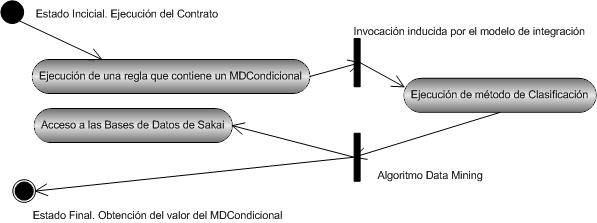
\includegraphics[width=6 in,totalheight=2 in]{Ch4/f4.jpg}
 % .: 0x0 pixel, 0dpi, nanxnan cm, bb=
\end{center}



Cuando, dentro en una NRR se utiliza un método para implementar
algunas de las técnicas de data mining (en este caso, la construcción de un
árbol de decisión por medio de un algoritmo TDIDT), queda conformada una
regla donde el valor de su condicional (el cual fue denominado MDcondicional)
responde –conceptualmente– a una estructura, en este caso: un árbol.
El vínculo entre las reglas del contrato y la efectiva representación del TDIDT
se concreta a través de una relación de agregación entre los parámetros del
contrato (representado por la clase “parámetros context-aware”, que se encuentra
dentro del subsistema que engloba el contexto, similar a la propuesta de
Schmidt, A., 2005) y la clase DMcondicionales (representada como una
generalización de subclases donde se distinguen las posibles técnicas de data
mining).

En la figura \ref{}, las componentes significativas para la integración de los
modelos se encuentran enmarcadas en color gris. La primera pertenece al área
de coordinación de contrato y mantiene la estructura original del modelo pro-

puesto en el proyecto “Obra abierta”. La segunda componente se encuentra
representada por una clase conceptual que simboliza las características y funcionalidades
de minería de datos, articuladas para cumplir los objetivos y
requerimientos propuestos.

\paragraph{Mecanismo de comunicación}

La figura 5 es una reelaboración significativa de integración arquitectónica
entre dos modelos (el framework e-learning y el modelo de minería de datos)
donde se muestran, además, relaciones salientes de dependencias entre objetos
de las distintas áreas. Por ejemplo, cuando un objeto perteneciente a una
herramienta5 de la aplicación atiende un pedido de un usuario, se comunica
con otro objeto (en este caso un objeto contrato, perteneciente al área de
coordinación de contrato) con el propósito de verificar la existencia de una
regla que determine cuáles son las acciones que se deben tomar, teniendo en
cuenta determinadas condiciones. Si alguna de las condiciones está representada
por un MDcondicional, entonces existirá una comunicación entre el
objeto contrato (que contiene la regla) y un objeto del área de minería de
datos. Esta cadena de eventos y relaciones entre áreas permite que un servicio
ordinario del framework Sakai se pueda enriquecer con información de contexto
recopilada con técnicas de minería de datos.

\paragraph{Caso de uso}

Retomamos un requerimiento similar al propuesto en la sección “Métricas
de interacción para ‘Obra abierta’ ”, y agregamos que el análisis de información
almacenada es utilizada como recompilación de información (datos) de
contexto.

En este ejemplo, cambiaremos pequeños aspectos de los requerimientos
originales para poder involucrar las técnicas de minería de datos como parte
de la implementación, refiriendo el caso sobre el entorno Sakai.
Supongamos ahora que volvemos a la hipótesis de contar con un dispositivo
hipermedial conformado con la arquitectura del modelo de integración y
además, la implementación del modelo de la figura 6. Sabemos que la herramienta
se encuentra configurada con un contrato (del tipo de la sección “Los
contratos context-aware”) conformado, a su vez, con una regla similar a la presentada
en la sección “Modelo de integración”.

Entonces, cuando un usuario alumno ingrese al foro y ejecute cualquier
tipo de servicios donde intervenga el contrato anterior, las prestaciones que
recibirá estarán supeditadas a los valores que se obtengan de la ejecución del
clasificador en base a la información obtenida a partir del registro de actividades
de la plataforma Sakai. Cabe aclarar que Sakai contiene un registro de
actividades al cual podemos acceder desde las tablas de las bases de datos.
La implementación y operatoria que implique la clasificación de los
datos desde los \textit{MDcondicionales} es responsabilidad del subsistema que
lo
implementa, respetando de esta manera la propiedad de independencia entre
los modelos de la integración señalada en la sección “Detalles del modelo de
integración”.

Si profundizamos en el tipo de relación que se establece a través de los
\textit{MDcondicionales} y tomamos como referencia el punto de vista del
usuario,
podemos caracterizar el flujo de ejecución de órdenes de la siguiente manera:
en la figura 6, podríamos considerar un estado inicial, en el que el sistema ejecuta
las reglas de un contrato que contiene una de ellas con un
\textit{MDcondicional}. Por medio de un método, se produce la invocación del
método
de clasificación que se encuentra implementado en el subsistema de minería
de datos (referenciado con la entidad “modelo externo” en la sección “El
contrato como conector”).

Las transacciones y estados que se suscitan son luego transparentes para el
modelo de integración y pueden resumirse en la ejecución de un algoritmo de
data mining donde se provoca un consulta a la base de datos Sakai y la ejecución
de métodos de clasificación (similares a los de la sección “Antecedentes
de técnicas de minería de datos”) para obtener el valor de verdad del
\textit{MDcondicional}, llegando, así, al estado final del ciclo de ejecución.


Con este tipo de configuración, la herramienta foro de Sakai adquiere
características context-aware y el agregado de la siguiente propiedad: los contratos
context-aware pueden ser modificados en tiempo de ejecución. Esto
quiere decir, que el mismo alumno, ante una nueva interacción con el foro y
bajo las mismas condiciones, puede obtener resultados diferentes en el caso de
que se hayan modificado las reglas del contrato. Además, la incorporación de
un subsistema para la aplicación de técnicas de minería de datos ofrece mayor
potencial expresivo para la construcción de reglas en los contratos.


Finalmente, sobre esta temática consideramos que el uso de un correcto
modelo para la implementación de técnicas de minería en la clasificación de
valores de contextos permite potenciar las soluciones creadas para los dispositivos
hipermediales dinámicos para educación e investigación. Es importante
entonces, que el grupo de diseñadores, expertos y desarrolladores sean competentes
en la utilización comprensiva de este tipo de técnicas.

\begin{center}
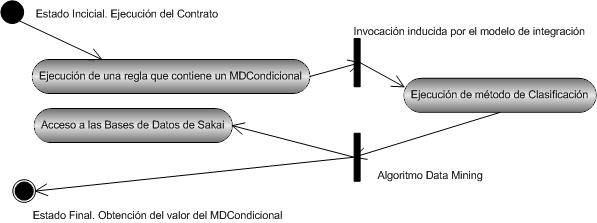
\includegraphics[width=6 in,totalheight=2 in]{Ch4/f4.jpg}
 % .: 0x50380343 pixel, 0dpi, 0.00xinf cm, bb=
\end{center}


\subsetion {Hacia la implementación de los CondicionalesDHD}

Con el objetivo de profundizar la visión sobre el diseño de dispositivos hipermediales
dinámicos, abordamos en este capítulo especificaciones técnicas que
justificaron la implementación y diseño de modelos de integración donde la
componente contrato adoptaba el rol de conector.
Observamos, entonces, que la base conceptual para que el contrato pueda
ser visto y manipulado en su diseño e implementación como una pieza de software,
se centra en el rol protagónico y responsable que debemos adoptar como
expertos diseñadores de dispositivos hipermediales dinámicos en el ciclo de
vida del mismo (diseño, implementación, uso).

Es a partir de esta nueva toma de posición, que la etapa de diseño adquiere
una dimensión activa centrada en la participación con la puesta en obra de
la teoría de coordinación de contratos context-aware.

Tomamos conciencia de que el camino hacia la implementación del
marco teórico propuesto demanda detenimiento para su comprensión, integración
de conocimientos de distintas disciplinas, diálogo interdisciplinar
para poder alcanzar claros criterios en la utilización del contrato y en la explicitación
de las reglas singulares que lo componen, configuradas en función de
los procesos educativos, investigativos o de producción que las susciten.
Teniendo en cuenta su poder expresivo, podremos desarrollar adecuadas
aplicaciones contextualizadas que nos abran la posibilidad de desarrollar nuestra
formación continua y creatividad, construyendo polifónicamente una singular
mesa de arena.


\section{Conclusiones}






% -- Archivo Cap\'{\i}tulo N� 5 --
%%--------------------------------------------------------------------------------------------------------------------
%------------------------------------------------- Chapter 5 --------------------------------------------------------

\chapter{Framework para la inyección de contratos sensibles al contexto en
entornos Web colaborativos} \label{cap:framework} \label{cap:6}
%\chapter{Framewrok to Implemet Context Aware Contract in E-learning

%\pagenumbering{arabic}


\section {Introducción} \label{intro}

A medida que el avance en la investigación y desarrollo de plataformas
e-learning brindan mejoras e innovaciones en herramientas
(videoconferencias, porfolios, wikis, workshops, etc.) y sus respectivos
servicios, crece la cantidad de posibles configuraciones de los espacios
e-learning. Estas configuraciones abarcan diferentes tipos de requerimientos
pertenecientes a las etapas de diseño, desarrollo e incluso exigen que el
espacio e-learning se adapte en tiempo de ejecución. A partir de estos
requerimientos se definen los procesos e-learning (que nosotros denominamos
Pe-lrn) \cite{tweb} de manera semejante a procesos de negocio en otro dominio de
aplicación. Al igual que los procesos de negocios en una Aplicación Web
convencional, los Pe-lrn están compuestos por transacciones Web \cite{}. En este
contexto, una transacción (o transacción e-learning) es definida como una
secuencia de actividades que un usuario ejecuta a través de una Aplicación
e-learning con el propósito de efectuar una tarea o concretar un objetivo, donde
el conjunto de actividades, sus propiedades y las reglas que controlan sus
ejecuciones dependen del Pe-lrn que la Aplicación debe brindar. Un ejemplo de
estrategia didáctica es la posibilidad de que un alumno acceda a determinado
tipo de material (vídeos, archivos, etc.)  dependiendo de sus intervenciones en
los Foros. Estos tipos de requerimientos resultan difíciles de implementar con
las actuales aplicaciones e-learning de extendido uso a nivel global. 

%Un ejemplo de un objetivo pedagógico es la posibilidad de que un alumno acceda a determinado tipo de material (vídeos, archivos, etc.)  dependiendo de sus intervenciones en los Foros. Este tipo de requerimientos son difíciles de implementar con las aplicaciones e-learning actuales \cite{libro}.

Las características funcionales de las actuales aplicaciones Web e-learning
(AWe-lrn), como Sakai\footnote{SaKai: Entorno colaborativo y de aprendizaje para
enseñar. Es de código abierto y está resuelto con tecnología Java. Véase
detalles en  \homedir{wwww.sakaiprojet.org})}, se basan en brindar navegación
entre páginas a través de links y ejecución de transacciones e-learning por
desde las herramientas (ej., Foros, Anuncios, Exámenes, Blogs, etc.) que
utilizan los servicios de la plataforma (ej., edición, manejo de audio y vídeo,
consultas, navegación, etc.). %La forma en que estos servicios son implementados
y la forma en que sus configuraciones pueden ser alteradas, son actualmente un
fuerte impedimento para implementar requisitos como el mencionado anteriormente.
%La configuración de estos servicios está fuertemente ligada a los aspectos
tecnológicos involucrados en las etapas de diseño y, principalmente, en la etapa
de desarrollo e implementación.% 

En el marco de los análisis efectuados podemos sostener que el proyecto Sakai
brinda una de las propuestas más consolidadas de diseño y desarrollo de entornos
colaborativos e-learning para educación, orientado a herramientas que se
implementan a través de servicios comunes (servicios bases). Por ejemplo, el
servicio de edición de mensajes es utilizado en las herramientas Foro, Anuncio,
Blog, PorFolio, etc. Más aun, otras de las características salientes de Sakai es
la versatilidad para su extensión y/o configuración. En efecto, Sakai permite
alterar ciertas configuraciones en tiempo de ejecución, por ejemplo,
instrumentar una nueva funcionalidad en un servicio base de Sakai. 


Sin embargo,  estas soluciones no pueden resolver aquellos Pe-lrn que involucren
cambios en el comportamiento de la relaciones entre un componente (cliente) que
ocasiona, a través de un pedido, la ejecución de un componente servidor
(proveedor). Estos tipos de cambios refieren a la capacidad de adaptación
dinámica del sistema \cite{kcomponent} extendiendo, personalizando y mejorando
los servicios sin la necesidad de recompilar y/o reiniciar el sistema. En este
trabajo se presenta un propuesta para la incorporación (agregado) de propiedades
de adaptación dinámicas a los servicios bases del framework Sakai, especialmente
diseñadas para implementar Pe-lrn definidos en el marco de \cite{ob} donde se
requieren nuevos aspectos de adaptación \cite{libro} en la perspectiva de los
Dispositivos Hipermediales Dinámicos en el campo del e-learning \cite{maxi} con
característica \textit{context-aware} \cite{libro5,libro6}. Se entiende por DHD
\textit{``a una red social mediada por las TIC en un contexto
físico-virtual-presencial, donde los sujetos investigan, enseñan, aprenden,
dialogan, confrontan, evalúan, producen y realizan responsablemente procesos de
transformación sobre objetos, regulados según el caso, por una coordinación de
contratos integrados a la modalidad participativa del Taller''}. (San Martín et
al, 2008) 

%Nuestra propuesta consite en lograr los niveles de flexibilidad dinámica mencionado incorporando a Sakai un framework para la coordinación de contratos. 


El resto de este trabajo se encuentra organizado de la siguiente manera:
Tras esta introducción se presenta una referencia conceptual del framework
contratos con características ``context-aware``, utilizados en el proyecto Obra
Abierta: Dispositivos Hipermediales Dinámicos para educar e investigar (Dir.
Dra. Patricia S. San Martín (Sección \ref{contrato}). Luego se describe la
macro-arquitectura de integración entre los frameworks de Sakai, la teoría de
coordinación de contratos sensible al contexto (TCCs-c), un modelo de contratos
context-aware y aplicaciones externas (sección \ref{macro}). Siguiendo,
se presenta un modelo de implementación de la TCCs-c a través del de patrones de
diseño (sección \ref{patron}). En la sección \ref{caso de estudio} se propone un
caso de estudio concreto. Finalizando con una
breve conclusión.


\section{Contractos con características sensibles al contexto} \label{contrato}

Nuestra propuesta de solución a los requerimientos mencionados sobre adaptación
dinámica comienza con la construcción de un modelo de contrato orientado a la
implementación de servicios sensibles al contexto. El uso de contratos parte de
la noción de Programación por Contrato ("Programing by Contract") de Meyer
\cite{Meyer} basada en la metáfora de que un elemento de un sistema de software
colabora con otro, manteniendo obligaciones y beneficios mutuos. En nuestro
dominio de aplicación consideraremos que un objeto cliente y un objeto servidor
``acuerdan`` a través de un contrato (representado con un nuevo objeto) que el
objeto servidor satisfaga el pedido del cliente, y al mismo tiempo el cliente
cumpla con las condiciones impuestas por el proveedor. Como ejemplo de la
aplicación de la idea de Meyer en  nuestro dominio de sistemas e-learning
planteamos la situación en que un usuario (cliente) utiliza un servicio de
edición de mensajes (servidor) a través de un contrato que garantizará las
siguiente condiciones: el usuario debe poder editar aquellos mensajes que tiene
autorización según su perfil (obligación del proveedor y beneficio del cliente);
el provedor debe tener acceso a la información del perfil del usuario
(obligación del cliente y beneficio del proveedor).

A partir de la conceptualización de contratos según Meyer se propone una
extensión por medio del agregado de nuevas componentes para instrumentar
mecanismos que permitan ejecutar acciones dependiendo del contexto. 

En aplicaciones sensibles al contexto \cite{Dey}, el contexto (o información de
contexto) es definido como la información que puede ser usada para caracterizar
la situación de una entidad más allá de los atributos que la definen. En nuestro
caso, una entidad es un usuario (alumno, docente, etc.), lugar (aula,
biblioteca, sala de consulta, etc.), recurso (impresora, fax, etc), u objeto
(examen, trabajo práctico, etc.) que se comunica con otra entidad a través del
contrato. En \cite{libro5} se propone una especificación del concepto de
contexto partiendo de las consideraciones de Dourish \cite{contexto} y adaptadas
al dominio e-learning, que será la que consideraremos en este trabajo. Contexto
es todo tipo de información que pueda ser censada y procesada, a través de la
aplicación e-learning, que caracterizan a un usuario o entorno, por ejemplo:
intervenciones en los foros, promedios de notas, habilidades, niveles de
conocimientos, máquinas (direcciones ip) conectas, nivel de intervención en los
foros, cantidad de usuarios conectados, fechas y horarios, estadísticas sobre
cursos, etc.


En términos generales, la coordinación de contratos es una conexión
establecida entre un grupo de objetos aunque en este trabajo se consideran sólo
dos objetos: un cliente y un servidor.



Cuando un objeto, cliente efectúa una llamada a un objeto servidor (ej.,
elservicio de edición de la herramienta Foro), el contrato ''intercepta'' la 
llamada y establece una nueva relación teniendo en cuenta el contexto del objeto
cliente, el del objeto servidor, e información relevante adquirida y
representada como contexto del entorno \cite{contexto}. Como condición
necesaria, el uso de  contratos no debe alterar la funcionalidad de     
la implementación de los objetos participantes, aunque sí se espera que altere
la funcionalidad del sistema.

A continuación se presenta un modelo conceptual resumido de contratos sensibles
al contexto. Se brindarán detalles sobre algunas de los componentes y relaciones
esenciales para la integración de este modelo con el framework Sakai y con los
módulos que instrumentan la coordinación de contratos \ref{macro}.

\subsection {Elementos de los contratos sensibles al contexto}

% %El contrato puede ser configurado por medio de diferentes mecanismos, desde el
% lenguaje cotidiano hasta un lenguaje de especificación formal, o un lenguaje
% basado en XML para los casos que sean necesarias especificaciones que puedan ser
% procesadas por máquinas. 

Un contrato que siga las ideas de Meyer contiene contiene toda la información
sobre los servicios que utilizarán los clientes.Para incorporar sensibilidad al
contexto nuestros contratos deberán tener referencias sobre algún tipo de
información de contexto para su utilización.

En el diagrama de relaciones entre entidades mostrado en la Figura
\ref{contratoca} se describen los elementos que componen elconcepto de contrato
sensible al contexto, especialmente para Pe-lrn.

\begin{figure}[!ht]
\begin{center}
	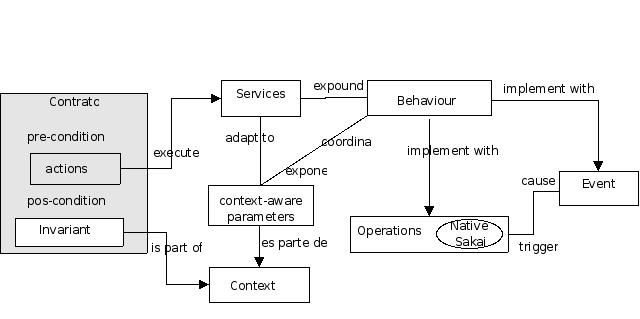
\includegraphics[width=5 in,totalheight=2.8 in]{Ch5/f1}
	\caption{\small \sl Modelo de un contrato context-aware} \label{contratoca}
\end{center}
         \end{figure}

El propósito de la presentación de este modelo de contrato sensible al contexto es identificar cuales son los componentes que lo componen y que serán referenciados en la siguiente sección para la implementación de un modelo de integración con el framework Sakai. 

La figura comienza con la representación de un contrato según Meyer donde se caracterizan los principales elementos que lo componen (pre-condiciones, acciones, pos-condiciones). La flechas salientes de la zona gris indican los dos tipos de relaciones que se debe instrumentar para incorporar un mecanismo que provea a los contratos la característica de sensibilidad al contexto. La primera de estas relaciones indica que desde las acciones del contrato se invocan a los servicios que provee un objeto servidor. La segunda relación se da debido los invariantes pueden depender de información de contexto. En la porción derecha de la Figura \ref{contratoca} aparecen las entidades necesarias para obtener contratos sensibles al contexto. Las explicamos a continuación.  

\begin{description}
\item[Servicios:] En esta componente se representan los elementos necesarios para la identificación de un servicios y clasificación de los servicios que pueden formar parte de las acciones de los contratos. Por ejemplo, nombre del servicio, identificadores, alcance, propósito, etc. Para más detalles consultar \cite{libro6}. El comportamiento funcional de cada servicio se expone a través de la componente \textbf{Comportamiento}.

\item[Comportamiento:] El comportamiento de un servicio se logra a partir de combinar operaciones y eventos que son representadas con el las componente \textbf{Operaciones} y \textbf{Eventos}. De la misma manera el servicio puede ser implementado a través del uso de eventos, representados con el componente \textbf{Eventos}, que puede lanzado operaciones del componente \textbf{Operaciones}. Por ejemplo, de acuerdo con los roles (ej., alumno, instructor, docente, etc.) asignados a un usuario de una herramienta involucrado en un Pe-lrn, en un determinado contexto del entorno (ej., si está en un espacio Foro) y del usuario (ej., si tiene permiso de moderador), la componente \textbf{servicio} brindan distintas funcionalidades (ej., editar un mensaje), que son instrumentadas por medio de operaciones concretas (ej., guardar un mensaje en una tabla) y/o a través de la publicación o subscripción de eventos. Las operaciones pueden ser de dos tipos: operaciones
que cambian el estado del sistema (tipo “update”) y/o operaciones que
proveen algún tipo de información sobre consultas  (tipo “query”). Estas operaciones pueden ser creadas creadas por el programador o utilizadas a partir de las operaciones provista por el núcleo del framework sakai (ej., adquirir el id de un canal de mensajes) usadas en los servicios bases (ej., el servicio de edición de mensajes). 

\item [Parámetros Context-Aware:] Se denomina \textbf{parámetros context-aware} a la representación de la información de contexto que forma parte de los parámetros de entrada de las funciones y métodos exportados por los servicios, estableciendo de esta manera una relación entre el componente \textbf{Servicios} y el componente \textbf{Parámetros contex-aware}. La influencia de estos parámetros en el comportamiento funcional de los servicios es representada a través de la relación entre los componentes \textbf{Parámetros context-aware} y  \textbf{Comportamiento}. 

\item[Contexto:] Este componente representa el contexto o información de contexto definida anteriormente en esta sección. Para nuestro modelo este tipo de información es utilizada de dos maneras diferentes: en primer lugar para la asignación de los valores que toman los \textbf{Parámetros context-aware}; en segundo lugar esta información puede ser utilizada para definir los invariantes que se representan en los contratos.
\end{description}



\section {Modelo de integración de Sakai con contratos} \label{sec:integracion} \label{macro} 

En esta sección se muestra un esbozo de la propuesta para incorporar a Sakai un mecanismo de coordinación de contratos sensibles al contexto, a través de la presentación de una diseño que describe la comunicación entre módulos \cite{arqModulos} y sus dependencias. En la figura \ref{macroarquitectura} los módulos son representados con paquetes UML y las relaciones  entre ellos por medio de flechas que indican comunicación y  dependencias. A su vez, en un segundo plano se muestra cuáles son las clases específicas de cada módulo y cómo se implementa la integración a través de estas.


El framework Sakai, representado en la figura \ref{macroarquitectura} por el módulo Sakai, está diseñado según una arquitectura de cuatro capas \cite{arquitectura}: La capa de \textbf{agregación} se encarga completamente de la  implementación de la interfaz con el usuario al estilo de las implementaciones de portales Web. La segunda capa denominada \textbf{presentación} tiene la responsabilidad de permitir la reutilización de los componentes Web (ej., "widget" que proveen calendarios, editores "WSYWIG", etc.). La tercera corresponde a la capa de \textbf{herramientas} donde reside la lógica de negocio de las herramientas Sakai que interactúan con el usuario (ej., Foro, Wiki, etc.). Por último la capa de \textbf{servicio} implementa los servicios Sakai bajo una Arquitectura Orientada a Servicios que serán utilizados por varias herramientas a través de API. 

Para nuestra propuesta de integración tendremos en cuenta únicamente servicios que componen laa capa de \textbf{servicios} pertenecientes a los servicios bases Sakai. Los servicios del núcleo Sakai serán envueltos mediante la coordinación de contratos, lo que se representa en la Figura \ref{macroarquitectura} con las referencias del \textbf{Módulo Sakai} hacia el \textbf{Módulo de Coordinación de Contractos}.


De esta forma, se logra controlar las invocaciones a los servicios del núcleo Sakai a través del \textbf{módulo} \textbf{Coordinación de Contratos}, quedando establecida una primer relación de integración. Esta misma relación es implementada a nivel de clases como una relación de agregación entre la clase \textit{Servicios Sakai} (correspondiente al módulo Sakai) y la clase \textit{Conector} correspondiente al framework de coordinación que será tratado en la sección \ref{patron} a través del uso de patrones de diseño.

\begin{figure}[!ht]
\begin{center}
	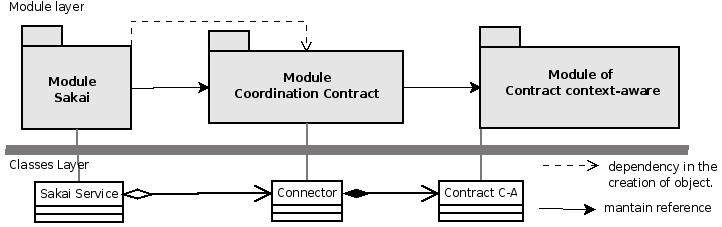
\includegraphics[width=4.5 in,totalheight=2.4 in]{Ch5/f2}
	\caption{\small \sl Diseño de la integración de Sakai con Contratos} \label{macroarquitectura}
\end{center}
\end{figure}

La última relación de integración se produce entre el módulo de \textbf{Coordination de Contratos } y el módulo de \textbf{Contratos Sensible al contexto} el cual fue  desarrollado en la sección \ref{contrato}. En este caso, la figura \ref{macroarquitectura} muestra cómo desde el framework de coordinación se estable una relación de composición entre la clase \textit{Conector} y la clase \textit{Contrato C-A} que implementa el elemento Contrato representado en la Figura \ref{contratoca} coloreada en gris.

De esta forma, instanciando dinámicamente diferentes contratos, Sakai presentará una flexibilidad en tiempo de ejecución que actualmente no posee y que es la que requieren los DHD. 
 

\section{Implementación de contratos en Sakai} \label{patron}

En las secciones anteriores se mencionó al contrato como un agente activo que se encarga de la coordinación de las componentes que lo integran. En esta sección se describe cómo este mecanismo fue implementado a través de una herramienta que permite modificar implementaciones de clases Java de los servicios Sakai para incorporarle mecanismos de coordinación de contratos sensibles al contexto, según el diseño mostrado en la Figura \ref{macroarquitectura}. Sin embargo creemos que antes es conveniente resumir brevemente otros intentos de proveer la flexibilidad requerida por los DHD.

Lograr este grado de flexibilidad es absolutamente necesario teniendo en cuenta que la implementación de estas clases, para los frameworks colaborativos e-learning como Sakai, no pueden ser modificadas (rediseñadas, reemplazadas). Para estos casos, la implementación de la TCCs-c proporciona un mecanismo que se distingue de propuestas existentes para el modelado de interacción entre objetos. 

\subsection {Niveles de flexibilidad de Sakai}

Diferentes estándares y frameworks de desarrollo de software basados en componentes e inyección de servicios fueron propuestos para mejorar la flexibilidad y adaptabilidad\footnote {La adaptabilidad en el sentido que se proponen en los sistemas hipermediales que permiten personalizarse (adaptarse) en función de los usuarios individuales (Henze, 2000).} de los sistemas e-learning Web, los más importantes son: CORBA, JavaBeans, Hibernate, Spring, JSF, RSF, etc. Sin embargo, ninguno de estos estándares proveen un mecanismo convenientemente implementativo y abstracto en donde se 
permita representar a las relaciones entre usuarios y servicios como un objeto de primera clase \cite{Meyer}. En este sentido, se implementa una solución utilizandos patrones de diseño que implemente características deseadas de la TCCs-c sobre la capa de servicios base de framework Sakai.

Desde un punto de vista implementativo, esta propuesta cambia la filosofía Java2EE-Sakai\footnote{Sakai mantiene la filosofía de desarrollo de Java2, de aplicaciones orientadas a servicios ("service-oriented) que pueden ser escalables, fiable, interoperable y extensible.} donde la incorporación de nuevas prestaciones de versatilidad para la configuración e implementación se logran a través de extensiones de clases, relaciones a liberías, técnicas de reflexión ("Reflection"), etc. 

En el siguiente diagrama de clases UML se muestra el diseño propuesto para incorporar coordinación de contratos sensibles al contexto en Sakai. A continuación explicamos  cada uno de los componentes y sus relaciones.


\subsection {Patrones de diseño para la coordinación de contratos sensible al contexto}

\begin{figure}[!ht]
\begin{center}
	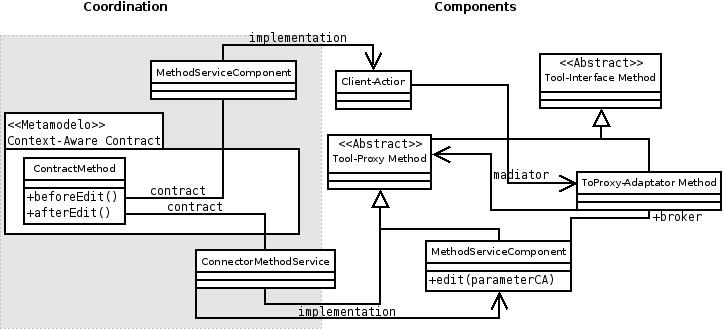
\includegraphics[width=5 in,totalheight=2.4 in]{Ch5/f4}
	\caption{\small \sl Diseño del modelo de integración} \label{contratos-patrones}
\end{center}
         \end{figure}

\begin{description}

\item[MétodoHerramineta\_Interfaz:] Como su nombre lo indica, esta es una clase
abstracta que define una interfaz común de los servicios de una Herramienta
provisto por \textbf{MétodoHerramienta\_Proxy}
y \textbf{MétodoToProxy\_Adaptador}

\item[MétodoToProxy\_Adaptador:] Esta es una clase concreta que implementa a un
intermediario manteniendo la referencia a la clase \textit{Método\_Proxy} para
encargarse de los pedidos recibidos. En tiempo de ejecución, esta entidad puede
indicar a \textbf{MétodoServiceComponente} que no hay contratos involucrados o
instrumentar una conexión entre \textbf{ConectorMétodosService} para que conecte
la clase real \textbf{MétodoServiceComponente} con el contrato
\textbf{ContractMétodo} en el que se encuentran las reglas de coordinación.

\item[MétodoHerramienta\_Proxy:] Es una clase abstracta que define la interfaz
que tienen en común \textbf{MétodoHerramientaToProxy\_Adaptador} y
\textbf{ConectorMétodoService}. La interfaz es heredada de
\textbf{MétodoHerramienta\_Interfaz} con el propósito de garantizar que ofrezca
la misma interfaz de \textbf{MétodoHerramientaToProxy\_Adaptador} con la cual un
cliente real debe interactuar (ej., un objeto que invoque el servicio de edición
de un Foro).

\item[EditServiceComponente:] Es la clase concreta  donde se encuentra la lógica
de la edición del Foro y la implementación concreta de los servicios originales
de Sakai.

\item[ConectorMétodoService:] Efectúa la conexión entre el contrato y los
objetos reales (en este caso \textbf{MétodoServiceComponente}) involucrados como
partes del contrato. De esta manera, no se requiere la creación o instanciación
de nuevos objetos para coordinar el mismo objeto real agregando o sacando otros
contratos. Esto es posible solamente con una nueva asociación a un nuevo
contrato y con la instanciación de una conexión con una instancia existente de
\textbf{ConectorMétodoService}. Esto significa que hay una sola instancia de
esta clase asociada con una instancia de \textbf{MétodoServiceComponente}.


\item [ContractMétodo:] Es la clase que cuya instancia genera un objeto de
coordinación que al ser notificado toma decisiones siempre que un pedido es
invocado a través de un objeto real.
Para los casos en que no haya contratos coordinando un objeto real, el diseño de
la figura \ref{contratos-patrones} puede ser simplificado y sólo las clases y
relaciones que no pasen por la zona del rectángulo gris son necesarias. La
introducción de un contrato implica la creación de las clases y relaciones
enmarcadas en la zona gris. La clase que implementa al contrato,  llamada
\textbf{ContractMétodo}, se encuentra representada dentro de la figura de un
paquete UML, llamado \textbf{Contratos Sensible al Contexto}, indicando su
pertenencia a un modelo subyacente descripto en la sección \ref{contrato}.
\end{description}

Este mecanismo de intercepción permite imponer otra funcionalidad en la
interacción entre componentes del llamante (por medio de su pedido) y del
llamado (a través de su respuesta). De esta manera, desde el aspecto tecnológico
se instrumenta la posibilidad de brindar un nuevo ``grado de libertad`` a los
servicios de Sakai, permitiendo establecer configuraciones propias de un DHD en
tiempo de ejecución.

Por lo expuesto, es válido reforzar la argumentación sobre las ventajas de esta
propuesta en comparación con las actuales soluciones tecnológicas basadas en
componentes y frameworks para la inyección y representación de servicios. A su
vez, se observa que el camino de su instrumentación es complejo debido a que se
deben generar (automáticamente) porciones de código y creación de nuevos
archivos código Java, a partir de los originales de la plataforma Sakai, que
deberán ser compilados y puestos en servicio para su operatividad. Cabe destacar
que los procesos de compilación y puesta en servicio de Sakai es efecutada una
sola vez, cualquier tipos de cambios y configuración serán impuestas a través
los contratos sensibles al contexto. 

La implementación de la coordinación de contratos en Sakai requiere del uso de
una herramienta específica para el dominio de aplicación (en este caso
aplicaciones e-learning) que modifica los archivos de código fuente Java que
implementan los servicios bases perteneciente al framework núcleo (similares a
los representados en esta sección), con el fin de incorporar la infraestructura
para trabajar con contratos de forma más o menos automática.

Para este propósito, se diseñó e implementó un prototipo experimental de una
herramienta llamada SwC ("Sakai with Contract") y un entorno de desarrollo que
permite instrumentar una metodología \cite{cacic,edutec} para la inclusión de
contratos en Sakai bajo la perspectiva de un DHD. El desarrollo de la
herramienta SwC está basada sobre el proyecto CED (Coordination Development
Environment)\footnote{CED: es el primer prototipo de una herramienta que
implementa el uso de la coordinación de contrato en aplicaciones Java. La
herramienta pertenece a ATX Software (www.atxsoftware.com);fue desarrollada
en Java y es de código abierto.} que implementa la coordinación de contrato a
través de un lenguaje llamado Oblog \cite{lenguajeoblog}. En este artículo no se
describen detalles técnicos de cómo la herramienta lleva a cabo la modificación
del código Java dentro de los distintos componentes de la arquitectura Sakai y
cuáles fueron las modificaciones puntuales efectuadas a partir de CED. 

%Las principales diferencias conceptuales entre CED y nuestra extensión parte de las propuestas enunciadas en la sección \ref{intro} y desarrolladas en la sección \ref{macroarquitectura} que ameritan un rediseño y agregados de módulos, algoritmos, interfaces, casos de uso, test, ejemplos, documentación, etc.


\section {Caso de estudio para la implementación de contratos} \label{caso de estudio}

En esta sección se presentará un caso de uso para ejemplificar las diferentes
etapas que se deben cumplimentar para lograr la inclusión de contratos en Sakai
bajo la perspectiva de los DHD, retomando la idea de incluir un contrato en los
servicios de edición de la herramienta Foro de Sakai.

Si bien consideramos importantes las observaciones realizadas sobre el por qué
de la necesidad de utilizar una metodología concreta para el diseño del contrato
referidas al lugar que ocupa dentro del flujo de ejecución de un Pe-lrn, qué
tipo de requerimientos satisface, cómo fueron relevados dichos requerimientos y
una especificación (en lo posible semi-formal) para su implementación, un
desarrollo más exhaustivo consta en otra publicación. Dicha metodología -llamada
UWATc- fue desarrollada en \cite{edutec}  para este mismo caso de estudio, y en
\cite{cacic} se amplían los detalles tecnológicos involucrados en su diseño. En
esta instancia UWATc brindará información sobre: cuáles son los servicios, en
qué clase (archivo Java) se encuentran representados (teniendo en cuenta el
flujo de ejecución) y cómo es configurado el contrato.

Nos centramos ahora en la última etapa del ciclo de vida de la configuración de
un espacio e-learning Web perteneciente al tiempo de compilación. En efecto, en
esta instancia el ingeniero de software cuenta con la información necesaria para
localizar los archivos de código fuente de la aplicación Sakai, los archivos de
configuración de los frameworks adicionales y demás configuraciones propias de
la herramienta para la inyección de los contratos.

Siguiendo  con el caso de estudio de las etapas anteriores, a continuación  se
muestra una porción de código Java correspondiente al código fuente original de
Sakai, en  donde se propone un método llamado \textbf{editMenssage}
correspondiente a la implementación del servicio edición de la herramienta Foro.
El siguiente fragmento de código fuente Java implementa una herencia de la clase
\textit{BaseDiscussionService} donde se encuentran las interfaces de los
servicios de edición correspondiente al núcleo del framework Sakai. 

\small \begin{verbatim}
import org.sakaiproject.discussion.api.DiscussionMessage; 
public class DiscussionService extends BaseDiscussionService{
public MessageEdit editMessage(MessageChannel channel, String id)‏{
return (MessageEdit) super.editResource(channel, id);}
\end{verbatim} \normalsize

Luego, a través de la herramienta SwC se crean archivos XML (similar a la
herramienta CED) para especificar las reglas del contrato que involucrarán
servicios implicados en el método \textit{editMensage} (Paso1). A continuación,
se ejecuta la generación automática de código para crear dos tipos de archivos
Java diferentes (Paso2). El primero (archivo 1) implementa las funcionalidades
que permitan las conexión con el Proxy (ej., \textit{MétodoHerramienta\_Proxy}
para nuestro caso de estudio); el segundo (archivo 2) implementa el conector
\textit{ConectorEditService} representado en la figura
\ref{contratos-patrones}. 

A continuación se muestran fragmentos de código que permiten una mejor
ilustración de las características adquiridas a partir de las modificaciones 
del código fuente de la aplicación Sakai a través de la herramienta.

\paragraph {Fragmentos del primer archivo - (archivo 1)}

\begin{enumerate}
 \item Se importan los paquetes correspondiente al framework de coordinación de
contratos (figura \ref{contratos-patrones}) y el framework context-aware (figura
\ref{contratoca})

\small \begin{verbatim}
package org.sakaiproject.discussion.impl; import java.util.*;
import cde.runtime.*; import obab.ca.*; // Framework context
public abstract class DiscussionService extends 
BaseMessageService implements 
DiscussionService,ContextObserver,EntityTransferrer,ForoInterface
\end{verbatim} \normalsize

\item  Métodos agregados por la herramienta para identificar las clases que van a ser interceptadas por el contrato.

\small \begin{verbatim}
protected CrdIProxy _proxy; 
private static Class _classId= Sakai.Discussion.class;
public static Class GetClassId() {return _classId;}
public CrdIProxy GetProxy() { return _proxy; }
public void SetProxy(Object p){if(p instanceof CrdIProxy && p instanceof 
DiscussionInterface) _proxy = (CrdIProxy)p; }
public void SetProxy(CrdIProxy p)  { _proxy = p; }
AccountInterface  GetProxy_Account(){if ( _proxy == null ) return null;  
return (DiscussionInterface) _proxy.GetProxy(_classId);}
\end{verbatim} \normalsize

\item Método que implementa la llamada del objeto cliente al Proxy

\small \begin{verbatim}
public long _getNumber(){new ComponentOperationEvent(this , "getNumber")_
.fireEvent(); return number;}
public messageEdit editMessage(MessageChannel channel,String id)‏{
new ComponentOperationEvent(this,"Edit").fireEvent();
return (MessageEdit) super.editResource(channel, id);}
\end{verbatim} \normalsize


\end{enumerate}

\paragraph {Fragmentos del segundo archivo - (archivo 2)}

\begin{enumerate}
\item Porción de código donde se importan las componentes de los frameworks, se
heredan las clases abstracta del los conectores y proxys. La clase del objeto
real \textit{MétodoService\_Componente}, según la figura
\ref{contratos-patrones}, se representa a través del atributo subject.

\small \begin{verbatim}
package org.sakaiproject; import java.util.*; 
import cde.runtime.*; import obab.ca.*;
public abstract class IDiscussionPartner extends 
CrdContractPartner implements CrdIProxy, DiscussiontInterface {
protected  Discussion subject;
\end{verbatim}\normalsize

\item Definición de los métodos abstractos para la conexión
(\textit{ConnectorMétodoService}, representada en la
figura \ref{contratos-patrones}), del contrato con el servicio.

\small \begin{verbatim}
public void SetProxy(Object p) {subject.SetProxy(p);}
protected Object GetSubject_Object() {return subject;}
public void ResetProxy() { subject.SetProxy(null);}
\end{verbatim}\normalsize


\item Métodos que permiten el acceso a los métodos que definen los servicios
(ej., métodos de la clase \textit{MétodoService_Componente})

\small \begin{verbatim}
protected Discussion GetSubjectDiscussion(){return (Discussion) subject;}
protected IDiscussionPartner GetNextPartner_Discussion(){
return (IDiscussionPartner)GetNextPartner(Discussion.GetClassId());}
\end{verbatim} \normalsize

\item Implementación por defecto de métodos definidos en la interfaces de los
servicios. A través del métodos \textit{GetSubjectDiscussion()}, detallado en el
punto anterior, se accede a los métodos creados por la herramienta en el primer
archivo.

\small \begin{verbatim}
public void messageEdit (double amount,Customer c)_
throws DiscussionException { IDiscussionPartner 
next = GetNextPartner_Discussion()
if (next != null) next.editMessage(amount,c); 
else GetSubjectDiscussion()._editMessage(amount,c);}
\end{verbatim} \normalsize

\item Implementaciones de los condicionales de la reglas de los contratos que se
encuentran en los archivos XML para configurarlos.

\small \begin{verbatim}
public CrdPartnerRules  messageEdit_rules(string texto,Student c) throws 
DiscussionException, CrdExFailure { return new CrdPartnerRules (this);}
\end{verbatim} \normalsize
\end{enumerate}

La generación de código automático a través de la herramienta presupone tener
ciertos niveles de conocimientos sobre: el lenguaje Java, aspectos de la
implementación del framework base Sakai y los frameworks que los componen; a
igual que experiencias en la compilación a través de Maven \footnote{Proyecto
maven: http://maven.apache.org/ref/2.0.4/maven-project/} de Sakai y las clases
modificadas-agregadas para el uso de contratos.

\section {Conclusión}

Fundamentados en el marco conceptual de los Dispositivos Hipermediales Dinámicos
para educación e investigación y en las actuales limitaciones observadas en las
plataformas e-learning sobre el grado de flexibilidad adaptativa en el sentido
de \cite{adaptativa} y \cite{kcomponent}), que pueda ser inducida por usuarios
expertos del dominio (ej., docentes) para el desarrollo de estrategias
didácticas efectivas para el logro de objetivos pedagógicos o investigativos 
planteados y, constando que dicha adaptabilidad no pueda ser enteramente resulta
por sistemas adaptativos inteligentes (ej., agentes, hipermedia adaptativa,
sistemas expertos, etc.), es que en este trabajo propusimos una implementación
de la teoría de coordinación de contrato en un framework específico sobre
sistemas colaborativos Web e-learning (correspondiente al proyecto Sakai)
brindando un modelo evolutivo conceptual y tecnológico. 
Partimos entonces, de las implementaciones de servicios y herramientas,
consideramos el agregado de componentes para la representación de cierta
información de contexto con aspectos context-aware para finalizar con la
incorporación de contratos para la coordinación de las interconexiones de los
servicios bases del framework original e-learning. De esta manera, el contrato
es una nueva primitiva prevista como una extensión de la noción de contratos de
B. Meyer \cite{Meyer} a la que se le adjudica el rol de coordinación de las
interacciones de los objetos.

El fin último de esta propuesta en desarrollo, se inscribe en brindar respuestas
tecnológicas efectivas a la necesidad de promover procesos educativos e
investigativos de interacción responsable entre los sujetos intervinientes en la
red sociotécnica del DHD, implementando la solución en los servicios cuya
prestaciones dependen -fuertemente- de reglas con estructuras volátiles cuyos
condicionales son influidos por el contexto (en el sentido de "Identificación
del contexto" desarrollado en el capítulo 5 \cite{libro} y manteniendo las
lineamientos sobre contexto fundados por P. Dourish \cite{contexto}). 

En este trabajo se propuso una implementación de la teoría de coordinación de
contrato en un framework específico sobre sistemas colaborativos Web e-learning
(correspondiente al proyecto Sakai). Se brindó un modelo evolutivo conceptual y
tecnológico, comenzando por las implementaciones de servicios y herramientas;
luego con el agregado de componentes para la representación de cierta
información de contexto con aspectos context-aware; finalizando con la
incorporación de contratos para la coordinación de las interconexiones de los
servicios bases del framework original e-learning. De esta manera, el contrato
es una nueva primitiva prevista como una extensión de la noción de contratos de
B. Meyer \cite{meyer} a la que se le adjudica el rol de coordinación de las
interacciones de los objetos.

Basados en nuestra visión de que las plataformas e-learning actuales carecen de
ciertos grados de flexibilidad adaptativa (en el sentido de \cite{adaptativa} y
\cite{kcomponent}), que pueda ser inducida por usuarios expertos del dominio
(ej., docentes, expertos en educación), para construir procesos educativos con
cierto grado de eficiencia. Donde, dicha adaptabilidad no pueda ser enteramente
resulta con sistemas adaptativos inteligentes (ej., agentes, hipermedia
adaptativa, sistemas expertos, etc.). Este requerimiento puntual hace referencia
a las necesidades de promover el tipo de solución que en este trabajo se
propone. Implementando la solución en los servicios cuya prestaciones dependen
-fuertemente- de reglas con estructuras volátiles cuyos condicionales son
influidos por el contexto (en el sentido de "Identificación del contexto"
desarrollado en el capítulo 5 \cite{libro} y manteniendo las lineamientos sobre
contexto fundados por P. Dourish \cite{contexto}). De esta manera se propone un
mecanismo para el diseño e implementación en tiempo de ejecución adaptada a un
tipo de aplicación e-learning Web.


% ----- Archivos de Ap\'{e}ndice -------------
%\fancyhead{}%
%\addcontentsline{toc}{chapter}{Ap\'{e}ndice A}
%\include{Appendix/appendix1}
%\addcontentsline{toc}{chapter}{Ap\'{e}ndice B}
%\include{Appendix/appendix2}
%\addcontentsline{toc}{chapter}{Ap\'{e}ndice C}
%\include{Appendix/appendix3}
%\addcontentsline{toc}{chapter}{Ap\'{e}ndice D}
%\include{Appendix/appendix4}
%\addcontentsline{toc}{chapter}{Ap\'{e}ndice E}
%\include{Appendix/appendix5}
%\addcontentsline{toc}{chapter}{Ap\'{e}ndice F}
%\include{Appendix/appendix6}

% --------- Archivo Bibliograf\'{\i}a -----------
\fancyhead[LE,RO]{\nouppercase{\textbf{\rightmark}}}%
\fancyhead[LO,RE]{}%
\addcontentsline{toc}{chapter}{Bibliograf\'{\i}a}
\bibliographystyle{plainnat}
\bibliography{bib}

% --------- Mis publicaciones ---------
%\addcontentsline{toc}{chapter}{Anexo}
%\include{anexo}
\end{document}
